%\bibliography{ref.bib}

\chapter{绪论}
\label{chap1}
\section{研究背景及意义}
近些年来,深度卷积神经网络对于我们已经不再是陌生的工具,它已经深刻地嵌入到我们生活中的每个角落,也一直在不断地发展解决人工智能领域的相关问题,
包括但不局限于目标检测 \cite{35,36}、图像分类 \cite{29,73},
这些发展成熟的神经网络已经可以很精确地识别出图像原有的语义信息和空间位置信息,但是大多数应用在公共场合的监控设施都是基于 RGB 图像的,而 RGB 图像对于光照、
光线明亮程度和获取图像视角等外界环境要求较为苛刻,一旦无法满足,则很有可能无法准确识别出个体而进行检测,而且在某些特定场合并不能很好地保护好被监测个体的隐私问题。
而且,多目标检测与跟踪是图像处理和视频监控领域的重要组成部分,尤其是在特定区域内的多人检测追踪和人流量监控任务在图像处理领域中更是受到了广泛关注,
其正迎合对于某些特定区域场所检测人流信息的安防需求,且这些信息可以帮助企业公司做出更好的判断和改进,从而带来更好的客户体验。
\begin{figure}[h]
	\centering
	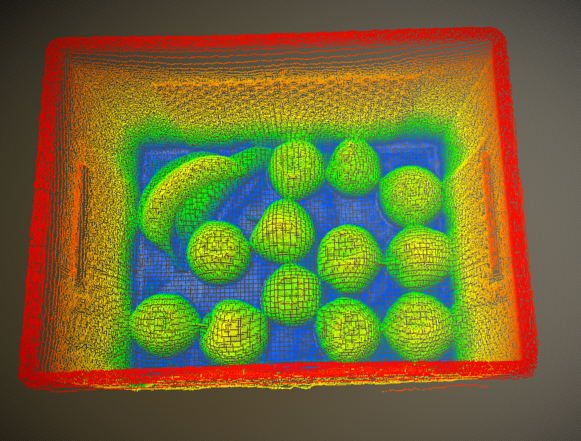
\includegraphics[width=0.67\linewidth]{chap1/depth_image.png}
	\caption{\ \ 具有层次变化的深度图像特征}
	\label{fig1-1}
\end{figure}

而近年来已有很多廉价的深度图像传感器出现,如 Kinect、Basler\ Blaze 等,这种基于飞行时间原理的 ToF(Time-of-Flight)
图像传感器具有成本低、结构轻量、准确度更可观以及稳定性更好的特点\cite{1},这也使得深度信息的获取和利用正在成为多人检测跟踪任务的关键突破点,
对比于 RGB 图像数据,深度图像数据具有更独特的深度信息和更好的辨识度,它可以通过接收发射出去的固定频率波来反馈不同深度平面的信息给检测算法(图1 - 1),以此深度特征来作为监测手段,
且 ToF 传感器并不受外界光照的影响,致使它可以在不同场景下稳定地完成任务,而不会产生意外情况。
因此我们选择在使用 ToF 传感器的基础上来进行整个监测系统的研究设计,这样可以很好地去除大部分外观差异对我们识别过程的影响,并且很好地保护用户隐私问题,
而如何使用深度图像特征来进行有效地监测追踪则是我们研究的重要组成部分。

除此之外,在实际应用中部署这些高性能、高复杂度的卷积神经网络时,我们还要考虑其所需要的大量存储空间和计算成本,这也是一个不可避免的重点问题。
以我们常见的标志性神经网络 ResNet-50\cite{73} 为例,其处理一张$224\times 224$的
RGB 图像需要至少 0.1 GB 的存储空间和 10 GFLOPs 的计算量,如此庞大的运算需要具有强大计算能力的运算处理单元、大容量存储空间的内存和长时间的大电量支持,
而这样苛刻的硬件条件是很难在一个轻便的移动端多目标实时监测系统上成功实现的。
因此,虽然深度卷积神经网络领域已有不少优秀的工作,但是为了研究设计一个简单有效的实时监测系统,我们需要找到性能和能耗的平衡点,因此除多目标检测和实时追踪外,
还需要进行深度卷积神经网络模型的轻量化,剔除神经网络中的大量冗余计算,同时使用硬件加速方法对底层存储运算做出优化,将整个实时监测系统部署到移动端硬件平台上,从而完成整个研究设计。

总的来说,此次研究的主要意义有两方面:
\begin{itemize}
	\item 一是研究深度图像的本质,利用具备信息隐私性更好、数据量更少特征的深度图像数据来完成限定区域内的多目标实时检测追踪和人流量监控,其中包括对多目标检测神经网络的优化和对多目标追踪算法的优化。

	\item 二是在于为日后的移动端开发应用进行预研和测试,通过在开发板上模拟现实运作环境来对整个多目标实时监测系统进行研究并改进,使得人工智能技术能够真正落地到实际应用中,而不再只是停留在算法层面的性能比拼,
	将重点转移到现实层面,也是为日后如何将整个监测系统集成到移动端而做出的研究铺垫,也希望对这部分内容的研究能有助于一体化设备的发展,设计出更高效、适用能力更强的人工智能硬件设施。
\end{itemize}

\section{国内外研究现状}

由于本研究中涉及不同的几个领域知识,分别为多目标检测、多目标追踪、网络模型轻量化与硬件加速三个部分,故下面将一一介绍这几种不同领域内容的国内外研究现状。

\subsection{多目标检测}
目前多目标检测研究的主要难点在于:复杂多变的背景信息、不同人之间的外观特征差异、不同个体的姿势状态随时在变化、检测到的目标自身首饰物品以及不同个体之间互相遮挡的问题等\cite{2},
在原有的基于 RGB 图像数据的多人检测算法中,人体轮廓、外观和衣服材质颜色等信息的多变性导致想要解决这类问题会很困难,其检测成功率也不尽如人意,
像是 Ramanan\cite{3}等人早期提出的一种只基于 RGB 图像的检测算法,其将人体的每一个肢体关节用长方形的检测框来对应,构建出足够多的人体肢体模型,再利用这些模型来进行目标检测。
Vera\cite{4}、Hsu\cite{5}、Perng\cite{6}等人使用前后背景分割的办法处理图像,在此类基于图像分割的算法中混合高斯模型 GMM(Gaussian of Micture Models)是常用的背景去除方法之一,
其余还有均值滤波和滑动均值滤波等,而后经过形态学算法处理,如腐蚀和膨胀等操作获得前景图像,再通过斑点检测等方式,依据斑点的形状、颜色、大小等标准进行筛选来获得人数和检测位置,
图像中的噪声去除大多利用中值滤波和高斯滤波处理。
García\cite{7}和 Ozturk\cite{8}等人利用图像边缘检测中的 Sobel 算子检测算法来获得人体头部的位置信息。除此之外 Gao\cite{9}等人还会利用头发的材质颜色信息来进行目标定位。

Bevilacqua等人\cite{10}首先利用 ToF 传感器获得 3D 模型来进行检测追踪人体,但是其算法有很多局限性,他要求进入图像传感器 FOV 内的人不能互相遮挡并且要按顺序一个一个进入监控区域以便产生 3D 模型。
一种基于单一摄像头的人体检测算法被 Mukherjee等人\cite{11}提出,其将摄像头置于头顶上一定高度,在进行前后景分离之后,
通过 Canny 边缘检测(Canny Edge Detection)算法对前景做霍夫圆(Hough Circle)检测,然后利用 Horn-Schunck 光流算法进行追踪,为避免人的轨迹被重复检测,
其提出了 STV (spatio-temporal validation),是一种先基于 AM(approximate median)进行背景分离,然后再计算时空域中两个不同轨迹的重叠比例,从而去除重复的追踪轨迹的方法。
Iguernaissi 等人\cite{12}提出用前后景分离方式检测识别出越过 LOI(line of interest)的人。
首先,设置一个垂直于地面的 Kinect 相机摆放在天花板上,然后设定一个 LOI ,利用深度图像检测出每一个通过 LOI 的人,其检测模块主要是利用前背景的深度差异来检测出人的出现和运动,
首先利用多张背景的平均值来设定初始背景图像,当背景确定好后,利用帧差法来提取前景,并使用高斯滤波使图像平滑,减少噪声。
之后通过计算提取前景中的黑色区域面积是否大于预设的单个人所占面积的阈值来判定这个前景是否是一个人。
Zhang 等人\cite{13}提出一种基于水由于重力作用会向附近的凹陷处流淌的现象的检测算法,其核心思想是因为人的头顶相较于其它身体部位与 ToF 传感器的距离最近,
所以对于在深度图像中检测出人所在位置的问题就等同于找到深度图像中的单个或多个最小值区域问题。此算法仿真雨水滴落的过程,向整张深度图像上按照均匀分布滴落水滴,
同时假设每个水滴的影响因子相同,并且水滴逐个滴落,直至流向最低点再进行下一次的滴落过程,于是每一水滴会向周围更低的方向流淌,直至不再流动,然后记录下这些区域最低点的水滴数量,
在之后把那些水滴数量超过一定阈值的区域最小值点记作一个人头中心点,从而做到检测人数的效果。为了减少算法的复杂度还可以另一个水滴携带多个水滴,而减少仿真水滴落下的循环次数,
因为在一个区域最低点的周围的水滴都会流向同一位置,故并不会产生太大差异,从而减少时间。还有基于此算法开发的应用\cite{14}。
还有一类基于运动检测的算法,其主要思想是利用视频流输入的前面一部分帧学习得到一个背景模型,而后利用不同的背景分割算法来获得检测目的,
Barnich等人提出 ViBe 算法\cite{15}、Hofmann等人提出 PBAS(Pixel-Based Adaptive Segmenter)算法\cite{16}、Hanzi Wang等人提出 SACON 样本一致性建模算法\cite{17}。
但这类方法有很多局限,首先图像传感器的位置不能有变化,而且只能检测运动的物体,无法识别静止的物体,多个物体重叠粘连也无法进行有效识别,天气和光线变化等因素也有很大影响。

还有一系列使用机器学习方法来进行目标检测的算法,一般先通过特定的特征描述子像是梯度方向直方图 HOG\cite{18}和尺度特征不变转换 SIFT\cite{19}的特征提取方法对图片进行特征提取,
可以是形状、面积、颜色、质地等,然后在图像中检测出人体并将其整理为训练集,再利用支持向量机 SVM(Support Vector Machines)、自适应增强 AdaBoost(Adaptive Boosting)、
随机森林(Random Forest)、级联分类器 Cascade 等机器学习模型进行训练实现人体检测。
Pang等人\cite{20}提出了一种基于 HOG 的特征提取方法,他提出来一种新的梯度分解方式并对梯度信息做更平滑的处理,
并减少了 CoHOG(Co-occurrence of Histograms of Oriented Gradients)的维度从而获得更鲁棒的结果,
而 Ahmed等人\cite{21}也提出了一种基于 HOG 的 r-HOG 算法,他提出在利用 HOG 提取图像特征之前,先将图像中的人通过所处位置与图像中心的距离和正余弦关系旋转,
然后调整截取框大小获得人的区域图像,以去除圆对称和较广 FOV 下的图像畸变影响,相较于 s-HOG 提升了近 40\% 的检测准确率,而且 95\% 的检测结果与真实人体中心误差在 36 个像素点之内。
而由于 HOG 特征只关注了物体的边缘和形状信息,后人又提出了针对目标表观特征的特征描述子,Piotr等人\cite{22}提出一种新的 ICF(Integral Channel Features)算法,
将特征提取过程包含共 10 个通道提取,由 6 个不同方向的梯度直方图、3 个 LUV 颜色通道和 1 个梯度幅值组成,从而获得更加多元的信息,再利用 AdaBoost + Cascade 进行多个尺度大小的分类器训练。
Felzenszwalb等人\cite{23}提出一种基于 HOG 的 DPM(Deformable Parts Models)特征提取算法,其利用一个粗调的大型模板来检测物体的整体位置特征,
再利用部分精度更高的小型模板来对应检测物体的各个部分的 HOG 特征,像人的头和肩、躯干、四肢,对这些部分分别进行特征提取,然后将组合起来的特征利用 LSVM(Latent-SVM)分类器实现检测。
Yan等人\cite{24}还有对 DPM 算法的优化工作,提出了多个针对 DPM 的加速策略。
Rauter\cite{25}提出,先通过设定一个期望的最小半径人头区域的滑动窗口,搜索整个深度图并利用基于非极大值抑制(Non-Maxima Suppresion)的方法来获得图像内符合预设面积阈值的最大值区域,
作为待定的人头区域,而筛选出来的待定区域的中心点未必都是人头的中心点,再利用一种类似 Mean-Shift 算法\cite{26}的 Gradient Climbing 算法来确定最后的人头区域,
之后利用一种新提出的深度信息特征描述子来提取整个区域内的平均深度值信息,利用直方图表示待定区域和周围区域的深度差异,
利用 LIBSVM 中使用径向基核函数(Radial Basis Function 简称 RBF)的 SVM 模块训练将样本映射到高维特征空间,从而利用训练好的分类模型检测出不同的人所在位置。
但此方法所提出的深度信息特征描述子仅在其所提出的应用场景下好于普通的 SLTP(Simplified Local Ternary Patterns)\cite{27}。
Carlos等人在\cite{28}中提出来一种分前后两个阶段的算法,其一是线下训练阶段,二是线上实时阶段。在线下阶段中会基于 PCA(Principal Components Analysis)训练出一个分为人、
带着帽子饰品的人和其他各种类场景的模型集合,而在线上实时阶段中,首先获得每一帧的深度图像,通过滤波消除噪声影响,而后寻找到各个区域最大值,并将每一个最大值区域扩展选定一个对应的 ROI,
包括肩膀和肢体,作为待定的人区域,然后对 ROI 进行特征提取,将获得的特征矩阵通过基于 PCA 的分类器来判定是否属于一个人或者其他的类。

随着深度学习席卷全球,在越来越多的领域中都会看到深度卷积神经网络的身影,而在图像处理领域更是如此,基于深度学习来检测目标的方法越来越多,其在人体检测应用场景下的高精确度是令人追捧的主要原因。
深度卷积神经网络第一次走进主流学术界视野是在 2012 年 ILSVRC 图像分类比赛中 Alex Krizhevsky 凭借著名的 Alexnet 卷积神经网络模型\cite{29}获得冠军,其颠覆了传统的特征提取方式,
通过大量的数据和训练自主学习特征,从而完成检测。而后在 Zhang等人\cite{30}改进了 ALexnet,提出一种整合分类、定位与检测的神经网络,将分类过程中提取的特征用于定位和检测,
只需要改变同一卷积神经网络的最后几层便可以完成不同的任务。
Girshick 在 DPM 算法在此领域僵持很多年之后,提出了一种里程碑式的卷积神经网络 R-CNN\cite{31},甚至在此之后多年的网络的更新迭代,像 Fast R-CNN、Faster R-CNN、YOLO 都有他的身影。
R-CNN 使用选择性搜索(Selective Search)算法在图像中选取一定数量的可能包含人体的区域候选框,进行缩放控制到一定大小(原文为$227\times 227$),
再利用 DCNN(Dynamic Convolution Neural Network)提取候选区域的特征向量,送入 SVM 进行分类得到类别信息,再送入全连接层回归得到检测结果。
Ertler 等人\cite{32}提出了一种基于 R-CNN 的检测模型,同时利用 RGB 和 Depth 图像信息进行训练,并利用 NMS 使其检测结果更加鲁棒。
He等人\cite{33}基于 R-CNN 提出了一种先对图像进行卷积,再对卷积神经网络后的特征图像标定候选区域并提取候选区域特征向量的 SPPNet,
与 R-CNN 相比只需要一次卷积操作,避免了重复计算卷积特征,大大减少了计算复杂度。SPPNet 使用 SPP(Spatial Pyramid Pooling)池化层,
在提取特征的操作中可以使用多个尺寸的标准进行池化操作并整合为固定尺寸的输出,而且 SSP 不在意输入图像的尺寸,因此可以很方便地将 SPP 后的图像特征输入到全连接层训练。
而后Girshick \cite{34}又在此基础上改进提出了 Fast R-CNN(Fast Region-based Convolutional Network),用 ROI(region of interest )Pooling 代替 SPP,
具体是在卷积获得特征图后,对图像中的每一个物体圈定一个 ROI,将此区域内的特征单独提取出来一个固定大小的特征向量,再送入全连接层,
而且 Fast R-CNN 将深度卷积神经网络和后面的 SVM 分类两个不同阶段整合到一起,使用一个新的网络直接做分类和回归,节省了大部分时间。
Ren 等人\cite{35}提出了 Faster R-CNN,其主要创新点是在主干网络中加入 RPN(Region Proposal Networks),此网络将整张图片的卷积特征共享给检测层,
几乎不需要花费额外空间来储存ROI特征。RPN 是一种 FCN(Fully Convolutional Networks),输入图像经过处理会获得不同的长方形检测框,并且带有判定此区域是何类物体的分数,
通过设置一定大小的滑动窗口,并取其中心位置为一个锚点,在每个锚点周围生成多个尺寸和长宽比的候选框,而后可以检测到多种不同尺寸的目标,
而且通过 NMS 基于候选区域的分类得分来抑制 RPN 重复的区域提取,通过交替训练 RPN 和 Fast R-CNN 来共享卷积特征。He 等人\cite{36}提出了 Mask R-CNN,
在 Faster R-CNN 对每个图像中的候选区域输出分类标签和检测框两种信息的基础上,又利用 FCN 输出一种图像中被检测物体区域的二值掩膜信息,
并且 Faster R-CNN 在做下采样和池化操作时都对特征图进行了取整操作,而作者通过双线性差值填补非整数位置的像素,从而获得了更精确的位置区域信息。

除了以上的这些分为候选区域生成和区域分类两阶段的网络,还有 YOLO\cite{37}这样的单阶段检测网络,其将目标区域预测和分类预测整合为一个神经网络,
在进行快速识别检测的同时保证较高准确率,YOLO 作者由 GoogleNet 的架构\cite{38}激发了灵感,提出了含有 24 个卷积层和 2 个全连接层,并利用$1\times 1$的卷积来做通道的缩量的网络架构。
YOLO 采用全图信息来进行预测,并且学习到的信息具有普适性,会更好的检测到相关物体,并可以实现实时检测任务。其首先将输入图像分为$S\times S$个网格,如果图像中物体的中心落在了某一网格,
那这个网格便负责此类物体的检测,每个网格都会预测物体区域的检测框和置信度,最终回归决定此区域内是否有检测物体并且属于哪个类,并利用NMS去除同一物体重复的预测。
而后作者改进了 YOLO 提出了 YOLOv2 和 YOLO9000\cite{39},YOLOv2 在 YOLO 的基础上使用 Batch Normalization 提升收敛速度(提升了2.4\%mAP),
High Resolution Classifier 来进行调整校正来适应更高分辨率的输入(提升了4\% mAP),移除全连接层使用卷积和锚点框(Convolutional With Anchor Boxes)来进行区域的预测,
提出了一种新的分类模型 Darknet-19,包括 19 个卷积层和 5 个 maxpooling 层,减少了计算复杂度,为了增强鲁棒性其采用多个尺度的输入来进行训练,
并利用 Fine-Grained Features获得更精细的特征信息,最终的 mAP 高达 78.6\%。除此之外,还提出一种检测和分类联合训练的模型,也就是 YOLO9000,
将 YOLO9000 同时在 COCO 检测数据集和 ImageNet 分类数据集上训练,使其可以检测到没有已标记类别的物体,YOLO9000 可以快速检测出超过 9000 个类别的物体,
总体 mAP 值为 19.7\%。作者在之后还发布了 YOLOv3\cite{40},此模型做了一些更多的尝试,像是使用了残差网络 Darknet-53 做特征提取,另外使用 FPN 结构实现了多尺度的检测,最高可达 33.0\%的mAP。
除 YOLO 系列外,Ahmad等人\cite{41}提出另一种基于深度学习网络的头顶视角检测算法,基于Liu W等人\cite{42}提出的 SSD(Single Shot multi-box Detector)模型,
此模型在室内和室外场景下分别可以达到 95\%和 94.42\%的 TPR。其利用原有图像和已标记好的实况检测框图像作为训练集输入到提前在 COCO 训练集上训练好的 SSD 模型中继续训练,
将其作为基本的检测和计数手段,将每一帧特征图像中的待定检测点筛选出来作为检测结果,但其检测结果的TPR会随着场景下人数的增多而下降,均值在 95\%,
FPR 会上升,均值在 0.2\%。还有Lin等人\cite{43}提出了 FPN(Feature Pyramid Networks),主网络采取 ResNet 残差网络架构,其特别之处在于其他算法的多尺度特征融合都是在在预测前进行的,
而 FPN 的预测是在多个不同尺度特征层上进行的,充分利用了低层特征高分辨率和高层特征的高语义信息。

\subsection{多目标追踪}
在目标检测追踪问题中,解决问题的方式一般是先检测出要追踪的目标,而后利用滤波进行追踪。
滤波的意义总的来说就是利用图像传感器获得的数据来确定可能的几种当前状态的置信度,通过滤波滤除错误的信息从而确定新的状态,反复迭代更新。
而其中最基础的非贝叶斯滤波莫属了,其余的滤波大多是基于贝叶斯滤波而优化的,贝叶斯滤波基于贝叶斯估计,其核心思想是通过一系列观测到的数据来估计无法直接观测得到的变量,
分为两个主要步骤,一是状态预测,二是校正更新,基于马尔科夫性,使用全概率公式展开进行状态预测,而后利用先验预测信息和当前观测信息进行校正更新,
在视觉追踪领域就是利用前几帧的图像信息来进行预测获得当前位置,并利用当前帧的观测数据来校正预测数据,并不断迭代更新当前状态,从而获得目标的轨迹。
R.E Kalman在之后基于此架构优化提出了卡尔曼滤波(Kalman Filter)\cite{44},是被广泛应用在计算机视觉追踪领域的算法,卡尔曼滤波其实是一种线性高斯系统应用贝叶斯方程求解的方式,
以最小均方误差为目的,利用数学递归方程进行状态预测和校正更新,其主要过程为:计算预测状态和真实状态之间的协方差矩阵,利用预测状态和协方差矩阵计算卡尔曼增益得到估计状态,
再计算估计状态和真实状态之间的协方差矩阵进行下一次递归\cite{45}。由于卡尔曼滤波的假设为线性问题,而在现实场景下的追踪情况又大多不是线性高斯系统,
故提出了应用于非线性非高斯系统的扩展卡尔曼滤波 EKF(Extended Kalman Filter)\cite{46}, EKF算法\cite{47}主要是利用数学方法将非线性函数进行一阶泰勒展开,省略高阶项,
求解雅可比矩阵获得线性化的函数,然后利用与卡尔曼滤波相似的方法计算预测状态和协方差矩阵等,迭代更新。Kadar等人\cite{48}提出另一种线性估计方法
无迹卡尔曼滤波 UKF(Unscented Kalman Filter),其以无迹变换 UT(Unscented Transformation)为基础,利用特定的采样算法将一些样本点逼近非线性高斯分布,
与 EKF 获得线性函数不同,直接对均值和协方差进行逼近,再将这些点代入非线性函数,从而估计出变量的均值和协方差,而后进行卡尔曼滤波估计。
Arasaratnam 等人\cite{49}也提出了一种解决非线性系统情况的容积卡尔曼滤波 CKF(Cubature Kalman filter),其基于三阶球面径向容积准则,将原有积分形式变换成球面径向积分形式,
提取一组数量与向量方程维度线性相关的容积点,使用这些容积点来逼近非线性高斯分布的状态均值和协方差,CKF 具有更高的精确度并可以更好的解决高维度的追踪问题。

除了优化的卡尔曼滤波,还有粒子滤波 PF(Particle Filter)\cite{50}也被用来解决非线性的追踪问题,粒子滤波算法基于由 Metropolis等人\cite{51}提出的蒙特卡洛采样方法,
解决了非线性非高斯系统中难以积分获得后验解析的难题,蒙特卡洛采样的思想是利用平均值代替积分求期望值,而又因为我们很难通过积分计算后验概率,所以可以利用蒙特卡洛采样代替计算后验概率,
我们只需要从后验概率中利用重要性采样方式采取一些粒子取平均值就可以确定状态。之后又利用统计学中的序贯分析方法应用到蒙特卡洛采样方法中,即 SIS(Sequential Importance Sampling)\cite{52},
其从重要性概率函数中生成采样因子,随着每次观测数据进行递推求得权重,以所有采样粒子的加权和来表示状态,这也是粒子滤波的原型。在 SIS 的过程中我们可以发现,随着递归更新权重,
其实前面很久之前的状态影响因子已经不大了,对于结果的影响几乎为零,于是 Gordon等人\cite{53}在1993年提出一种基于重采样的方法 SIR(Sequential Importance Resampling),
其提出先通过计算粒子的权重和再根据各个粒子的权值进行重采样,通过对粒子的重要性概率密度函数作筛选,将那些权重很小的粒子去除,并重复采样权重较大的粒子,就可以获得更鲁棒的结果。
除了利用各种滤波进行追踪之外还有一类利用核密度估计的算法,像是 Mean-Shift 算法,其思想基于由 Fukunage在1975年提出的一种估计无参密度梯度的方法\cite{54},
而之后 Cheng在 1995年\cite{55}提出了 Mean-Shift 均值漂移算法,不需要任何先验数据而只依靠当前状态的特征空间中样本点进行密度估计,新定义了核函数和权重系数,
利用核函数使偏移值对偏移向量的贡献随样本与偏移点的距离的不同而不同,使不同样本的权重系数不同,在采样充分的情况下,能够渐进地收敛于任意密度函数,
所以说应用在目标追踪领域就省去了前面提到的先验概率的计算问题。Comaniciu\cite{56}在2000年首次将 Mean-Shift 算法应用于视觉目标追踪问题,其以图像的颜色和质地为追踪的特征,
通过计算上一帧的目标模型和当前帧中目标候选模型的直方图特征,并基于巴氏系数判断相似性决定是否属于同一个目标,并迭代更新目标模型,从而完成追踪。
由于我们想让目标区域内的分散点对偏移向量的影响的权重根据距离的远近而有所不同,故Comaniciu又做出了进一步尝试\cite{57},
利用核函数对要提取的特征直方图进行加权获得相应的目标模型和候选目标模型,再基于巴氏系数来进行相似度估计,进行目标的定位和模型更新,为了对应不同时刻场景下目标的大小可能不同的问题,
每次选择最佳估计的时候,将核函数的带宽用三种不同尺寸(前一帧保存模型的带宽递增 0.1 倍)代入分别求解,并在最后保留拥有最大马氏系数的解值作估计进行迭代更新。
还有之后基于 Mean-Shift 的改进算法 CamShift(Continuously Adaptive MeanShift)\cite{58},顾名思义就是连续自适应的 Mean-Shift 算法,其先在视频序列中选择目标区域,
再利用提取的色彩直方图特征,利用 Mean-Shift 收敛估计位置并确定新的区域,反复操作进行追踪,所以当目标大小尺寸发生变化时可以随时调整以适应新的目标估计。
还有在 2016 年 Bewley\cite{59}提出的 SORT(Simple Online and Real-time Tracking)多目标跟踪算法,其主要有三部分组成:目标检测、卡尔曼滤波、匈牙利匹配。
在目标检测阶段使用 FrRCNN(Faster Region RCNN)网络,也是一个二阶段检测网络,先通过提取特征确定候选区域,而后分类进行检测。然后利用卡尔曼滤波对目标估计和实际观测进行递归推导,
并且使用匈牙利算法基于IOU距离对当前估计值和前一帧的实际观测值进行数据关联确定最佳估计,从而更新最新的目标位置,如果匹配成功则成功获得轨迹,
对于没匹配到的当前估计则认为目标在当前帧丢失,而没匹配到的前一帧观测值记为新出现的目标,而且基于 IOU 可以解决部分遮挡的问题。而在之后 Wojke 等人提出了基于 SORT 的 DeepSort 算法,
其应用卷积网络进行检测,并通过引入马氏距离和余弦距离两种不同度方式,经 IOU 匹配和级联匹配方式进行二者之间关联,利用 re-id 领域的模型解决了物体遮挡的难题。

除此之外,Avidan\cite{60}提出一种将 SVM 和光流法结合起来的追踪算法,其通过学习前背景之间的差异来进行分类追踪,
并在之后基于 AdaBoost 的多尺度特征选择思想\cite{61}提出将一个弱特征分类器和一个强特征分类器结合,来应对检测物体外观变化的问题。
Grabner等人\cite{62}提出 OAB 模型,其利用基于 AdaBoost 的多尺度特征选择算法 On-line Boosting 来对输入样例进行在线学习,在训练的同时不断更新整合检测物体的外观特征,
使算法最大化的识别出物体与背景的不同特征,Hager等人\cite{63}利用基于几何和光线变化的算法来对整个预测区域进行追踪,同时又因为作者使用图像中可以很快计算的特征如:
类哈尔小波、方位直方图等(Haar-like wavelets、orientation histograms),可以达到实时追踪的效果。Ross 等人\cite{64}为了改变利用固定外观特征做检测模型的局限性,
基于增量 PCA 算法提出了 IVT 增量视觉跟踪器,利用之前若干帧的子空间图像表示,将当前子空间的图像使用 PCA 处理,获得均值和特征向量并更新子空间模型,
通过计算特征子空间与目标的中心距离进行跟踪。Babenko等人\cite{65,66}提出了 MIL(Multiple Instance Learning)实时跟踪算法,其使用基于 MIL 的外观模型,
每一帧先对运动模型进行判断,所谓运动模型就是上一帧中检测到的图像周围一定距离内会生成很多 patch,通过外观模型判别分类,并利用贪心算法将新目标的位置定为离得最近的 patch,
在每一帧确定了新的位置后就会对外观模型和判别分类器进行更新,从而可以实时的更新物体特征,重复这样就实现了目标的跟踪。Mei等人\cite{67}提出$\ell_1$跟踪器,其追踪模块基于粒子滤波,
将追踪转化为稀疏估计的问题,在得到候选目标区域后,将目标区域向前几帧和若干人为设置的噪声进行$\ell_1$约束的稀疏投影,如果投影区域限制在前几帧的相应区域,则认为是相似度高,
若是投影在噪声区域,则认为是相似度低,利用稀疏投影后的残差来确定候选区域的相似度,通过比较是否大于阈值来确定是否为同一目标并用新的位置信息更新前几帧的保存图像,
从而达到追踪的目的,但是该方法的计算复杂度较高,从而不能应用于实时的场景。K.Zhang等人\cite{68}提出一种基于压缩的算法 CT(Compressive Tracking),
作者采用非适应性的随机映射来保留检测物体的图像特征空间结构,并使用非常稀疏的测量矩阵从图像的多尺度特征空间中提取特征、建立外观模型,再对前景物体和背景图像使用同一个稀疏矩阵进行压缩,
对压缩区域利用朴素贝叶斯分类器进行追踪并更新模型信息,从而达到实时跟踪的效果,此算法不具备多尺度适应性,且对运动情况复杂的情况并不鲁棒。 
Hare等人\cite{69}提出一种基于结构化输出预测的自适应追踪架构 Struck(Structured Output Tracking with Kernels),
其特别之处在于相较于利用先训练得到分类器再输出分数进行检测的方法,直接训练出一个预测函数进行检测,在 SVM 输出空间中直接通过核函数处理获得类别的判定,
节省了很多计算还避免了错误判断对于之后信息更新的影响,并引入了预算机制来对 SVM 维持的向量数做限制的 kernelised SVM,通过设置较小的向量数从而达到实时追踪的目的。
Zhong等人\cite{70}提出一种基于稀疏性协同模型的目标跟踪算法,为解决追踪时外观模型变化的难题,其使用将整体样板和局部表示结合的鲁棒的外观模型,
并提出了一种稀疏的分类器 SDC(sparsity-based discriminative classifier),通过计算信任值的方法,使得前景比背景获得更高权重,
还提出了一种稀疏的生成物体表示的模型 SGM(sparsity-based generative model),通过灰度直方图信息,将每个图像块的空间信息和遮挡情况考虑进去,
之后综合最新的观测和原始样板更新外观模型减少漂移现象并基于粒子滤波跟踪。Xu等人\cite{71}提出另一种结构化局部稀疏的外观模型,利用对齐池化方法可以在利用好物体的空间信息和局部信息,
大大改善了遮挡问题,通过对每个局部的 patch 池化获得的信息也可以帮助解决遮挡和定位问题,并提出了一种结合增量子空间学习和稀疏表示的模版更新策略,从而适应外观信息的变化。
还有对之后研究很重要的 KCF 算法,由 Henriques等人\cite{72}提出,KCF 将滤波的思想发挥到极致,
对图像矩阵与循环偏移矩阵相乘,产生很多偏移后的矩阵样本,而后将所有样本存在一个矩阵中而产生一个循环矩阵,再将样本空间通过离散傅立叶变换变换成为对角矩阵,
将计算复杂度降低为O(n $\times$ log(n)),并利用核函数(点积核、多项式核、径向基核及高斯核)将低维的非线性问题转化为高维的线性问题,再通过相关性滤波进行回归。

\subsection{网络模型轻量化与硬件加速}
近年来,深度卷积神经网络被广泛应用在图像分类、目标检测等领域,并取得了巨大的成功,但是与之出现的重要问题之一就是神经网络的计算参数量的庞大,
而模型轻量化的中心思想就是在设计网络结构的过程中,提前考虑网络的结构是否冗余或者在实践过程中测试不同网络结构的效果,从而改变网络结构直接设计出更加高效、结构更紧凑的网络模型,
来避免冗余的参数计算过程,值得注意的是此模块并不属于网络模型压缩领域,但确实可以起到加速网络的作用,甚至很多模型压缩的方法也会与此类模型轻量化的方法进行横向对比。
在轻量化模型领域首先做出尝试的要属 SqueezeNet\cite{74},由斯坦福和伯克利大学的几位联合作者共同提出,SqueezeNet 主要结构由两个模块组成,第一个模块称为 squeeze 卷积层,
其由一些$1 \times 1$的卷积组成,在这一层中对输入特征进行降维处理;第二个模块称为 expand 卷积层,其有一些$1 \times 1$和$3 \times 3$的卷积共同组成,此模块对之前降维后的特征进一步进行特征提取,
最终结合Deep Compression\cite{75}中的延迟缩减采样方法,使不同卷积层共享权值来减少权值存储参数,并同时保持原有神经网络模型的检测精度,
此方法甚至可以将 240 MB 大小的 AlexNet 的模型在 6 bit的情况下压缩到 0.47 MB,有整整 510 倍。
而后大名鼎鼎的 Google 也提出了所研究的轻量化模型系列方法 MobileNet,MobileNet第一次出现是在 2017 年,其主要思想是基于深度可分离卷积\cite{76},
此类卷积将特征信息从空间维度和通道维度分开,首先利用深度卷积的方式进行空间维度上的特征提取,再利用逐点卷积的方式在通道维度上处理经前者提取的特征来进行信息的融合,
极大地减少了网络参数量和浮点运算数。在此之后,又在 2018 年提出了 MobileNet v2,在 v2 中主要提出了两个改进点,分别是倒置残差模块和线性激活函数\cite{77},
我们知道,当低维信息映射到高维,经过 ReLU 后再映射回低维时,若映射到的维度相对较高,则信息变换回去的损失较小,
若映射到的维度相对较低,则信息变换回去后损失很大,故在逐点卷积后使用了线性变换,其作用是将输入映射回低维空间,而且在深度卷积层前添加逐点卷积层,也就是倒置残差模块,
利用这两种方法,可以减少因非线性激活而导致的信息丢失。而后在 2019 年又提出了 MobileNet v3,在 v3 中其利用 MnasNet 和 NetAdapt\cite{78}
这两种 Auto ML 技术来对网络结构进行初略搜索、强化学习以及微调来改善模型结构和计算效率。
在这之前的 2018 年其实还有另一系列网络结构 ShufflNet 被提出,首选是 ShuffleNet v1\cite{79},其中心思想是通过通道混排的操作来加强不同通道分组之间的特征信息交互,
从而省去融合各通道之间特征信息的冗余计算量。而 ShuffleNet v2\cite{80}则是提出了四条轻量化网络设计准则,包括:输入输出通道数相同时,内存访问量 MAC 最小、分组数过大的分组卷积会增加MAC消耗等,
从网络模型在硬件中应用场景出发,考虑其计算的最佳方式来设计更加紧凑的网络模型。
Kai Han 等人又提出了利用廉价卷积\cite{81}来对几组卷积特征进行一系列计算量很少的线性变化从而获得更多卷积特征的方式来节省计算资源从而获得原本的卷积效果。
同时在此类轻量化模型网络结构的末尾可以加入 CA 注意力机制的模块来提升整体模型的检测和分类效果。
CA 注意力机制由 Qibin Hu等人\cite{82}在 2021 年提出,CA 注意力机制在通道注意力的基础上兼顾位置信息,将通道注意力和空间注意力很好的融合,
相较于之前只考虑空间注意力的 SE 模块和将二者分离的 CBAM 模块效果更加鲁棒。

除此之外,我们知道,计算机中的数据存储都是利用物理地址上的内存空间使用一定长度的比特位表示,包括八位、十六位、三十二位、六十四位等,而硬件端的量化加速也是沿着此思路,
通过减少表示参数的数据位数来实现神经网络模型的压缩加速,量化一般情况分为两种,一种是非线性量化,另一种是线性量化,其差别在于量化过程的映射点间隔是否均匀。
像 Lin等人\cite{83}提出一种基于信号量化噪声比的方式对模型进行定点量化,除此之外还有 Vanhoucke等人\cite{84}则是将模型中的权重映射到离其最近的离散点进行量化、
Jacob等人\cite{85}提出在训练过程中插入伪量化操作来对模型进行 8 比特量化操作。另外,Chen等人\cite{86}在研究中设计了一种哈希网络,该网络利用简单的哈希函数将模型的权重进行分组后再进行参数共享。
另外还有 Gong等人\cite{87}也是对权重进行Kmeans聚类、Han等人\cite{75}通过在训练过程中将权重自动进行聚类,再利用哈夫曼编码的方式对聚类进行中心编码。
这种非线性量化方式可以有效降低数据存取的带宽需求,但在实际应用中算法通常需要先对数据解码,这会花费很多额外的时间,从而导致此类算法只能在特定的硬件平台下进行网络加速,比较受限。
与之相反,线性量化的量化点间间隔均匀,这种特性使得此类算法可以直接将量化后的网络用低位运算器进行运算,带来很明显的加速效果。
像是Gupta等人\cite{88}就使用 16 位定点数来代替原来的 32 位浮点数,减少了网络推理过程中的内存占用从而加快了计算速度。
还有一些特别的二值量化神经网络\cite{89,90},其计算速度虽然非常快,但是模型准确率与原未压缩模型有一定差距,因此还不能应用到现实中。

\section{本文研究内容}

本文研究的重点主要是基于深度图像对限定区域内的多目标进行检测追踪和统计人流量信息等处理,并搭建从 ROS 调用 ToF 传感器获得数据到算法检测追踪输出信息的端到端实时监测系统,
而后在硬件开发板上移植测试整个监测系统,做出优化使得复杂的检测神经网络能够在算力有限的开发板上实时运行,为日后人工智能移动端应用的集成开发做算法研究铺垫。
尽管目前的部分深度卷积神经网络已经可以很好地解决多目标检测追踪问题,但还是仍然存在着以下几个方面的问题:

\begin{itemize}
	\item 大部分检测算法都是采用 RGB 图像数据,利用不同的前背景分割手段获取目标前景,从而进行检测,但这类方法有很多局限,对于多个目标之间的间隔距离要求较高,
    如果多个物体重叠粘连则无法进行有效识别,而且,多个目标之间通常会有肢体接触,在图像中会呈现出奇奇怪怪的形状,导致误检。在这其中,部分算法专门基于物体的运动性特征进行检测,
    虽然检测精度上有所提高,但也有很多限制,首先图像传感器的位置需固定,不能有变化,而且只能检测运动的物体,无法识别静止的物体。
    除此之外,由于是 RGB 图像传感器,天气和光线变化等因素对所能获取的图像数据也有很大影响。
    因此我们在此问题上选择通过 ToF 传感器获取的深度图像数据,其可以有效地解决光线和人体外观服饰的动态影响,并在不同的视角中选择顶部视角来避免部分目标间遮挡从而导致的误判问题。

	\item 当前的追踪算法一般是首先通过算法检测出所要追踪的目标,而后利用各种滤波器进行追踪,滤波器的作用总的来说就是利用图像传感器获得的数据来确定几种可能存在的当前状态的置信度,
    滤波通过筛选掉错误的状态信息从而确定新的状态,反复迭代更新,最终完成对目标的追踪。除此之外,追踪算法对于多目标的应用则是比单目标追踪情况复杂得多,由于区域内有多个目标存在,
    如何区分每一帧中检测到的目标是否是新进入监测区域的目标以及如何确认检测目标和已确认轨迹之间的所属关系是一件较为复杂的事情,其影响因素极为繁杂,
    比如,不同目标之间相似度过高,又或者同一目标在不同时间做出不同动作和移动方式,
    又或者多个目标之间出现相互遮挡的情况从而导致迭代更新的过程中出现误判,更多像是检测目标的外观特征多变等等这些人类目标所特有的问题都是难以完美解决的。

	\item 大部分使用深度卷积神经网络的检测算法虽然检测精度和普适性都比传统算法要高,但是随之而来就会出现计算复杂度过高的问题,
    而在各项算力较弱的硬件平台上部署相关应用更是难上加难,故如何在现有基础算法上使得模型轻量化且不会缩减过多算法检测精度使我们重点要研究的问题。
    传统的机器学习算法和深度卷积神经网络算法的所需算力都是极高的,普遍需要 GPU 这种专用的图形处理器来进行运算,但是在普通的硬件设施上是很难达到相同的计算力的。
\end{itemize}
	
针对上述问题,本文总结了目前应用较为广泛的多目标检测及追踪算法,对其中的关键技术进行深入研究和讨论,基于实验目标进行相应的研究设计和实验改进,
并提出解决方案,完成整个检测追踪算法研究和实时监测系统开发的过程。

本文具体的研究内容包括:

\textbf{基于深度图像特征的卷积神经网络多目标检测算法}

传统的多目标检测算法普遍基于图像的前后景差别来进行分辨检测目标,常见的是利用各种滤波器和数字图像形态学处理操作结合来进行目标前景的提取,再通过斑点检测等方法来区分不同大小、
形状、材质的斑点获得目标位置信息,还有通过光流法等基于目标运动形态的不同和变化来进行检测的算法研究,这类算法主要是基于物体运动过程中每帧图像的形态和位置差异来获检测目标的信息,
但是受外观特征的变化影响太大,因此为了解决此问题,我们选择深度图像来进行研究,深度图像可以给我们很好的人体外观深度特征,这种特征是渐变的高度,从而避免了人体表面的服饰、
不同颜色等影响,可以很好的检测到人体自身特征。虽然我们已经有 Waterfilling 算法可以通过八邻域的方式计算人头位置信息,但是其准确性并不鲁棒,
对于不同数据集还是有部分差异的,在部分数据集中只能达到 98\% 左右的准确度,从而我们为此提出一种基于深度图像来进行深度卷积神经网络训练的检测方法,该算法从深度特征入手,
利用卷积神经网络对深度图像进行多重处理,从而获得目标的位置信息,其精度可以达到 99.4\%,且在多个不同数据集上(包含网络公开数据集和实验室单独采集的两个数据集)进行测试,
都达到了目标精确度上下轻微浮动的结果,区间为 97.8\% $\sim$ 99.4\%,这些实验也证明了整个算法的有效性和泛化性。

\textbf{基于深度图像特征的多目标追踪算法}

在多目标追踪领域有很多优秀的滤波器方法被提出,但其中应用最广泛的当属卡尔曼滤波,卡尔曼滤波是一种高效的自回归滤波器,它能在具有诸多不确定性情况的物体状态的情况下预测估计动态系统的状态,
被广泛应用在动态定位和卫星导航中,而且不像普通的追踪算法保存大量侦测物体动态位置信息浪费存储空间,卡尔曼滤波只需保存前一帧的具体信息即可,而后通过自回归,
利用原状态估计和已知外界影响偏移值更新下一帧的状态估计,从而完成整个过程的跟踪,而其占用内存和运行速度的高效率特性都是我们完成设计整个实时监测系统所必需的条件。
且针对于我们检测所使用的深度图像信息,需要研究并设计更为合适的追踪算法来进行轨迹和检测之间的关联匹配,如何充分利用深度信息特征、避免多个物体之间的遮挡影响,
以及如何应对多目标外观之间的不同差异和运动状态的更新而导致的形态变化都是追踪算法中需要面对的亘古不变的难题。对于此问题我们最终采用以DeepSort算法作为基础的优化多目标实时追踪算法来完成监测系统的实时追踪模块,
并且利用顶部视角的深度图像来避免大部分遮挡问题,很好地减少多目标之间遮挡导致的误判情况,并且使用深度图像信息我们可以很好的辨识不同个体之间的形态差异,
正如没有一片相同的树叶一样,我们个体之间的高度值变化也是极其独特的,并且在使用ToF深度图像传感器的前提下,我们可以忽略天气、光照等外部环境的影响,
从而不需改变相机设置条件即可从一而终地完成整个监测系统的设计部署,且整个监测系统的实时帧率可以达到 50 $\sim$ 65 FPS。

\textbf{联合多应用场景下的人体检测追踪的网络轻量化和加速以及完整系统的硬件实现}

任何需要深度卷积神经网络的算法都需要大量的存储空间和强大的运算设备,但是这些硬件需求在普通的开发板、人工智能芯片和移动端设备上都是不现实的,很难在移动端框架下实现的。
本文针对前文提出的一体化多目标检测追踪算法,应用并比较多种模型轻量化方式,在此基础上再利用tensorrt 量化手段优化硬件设备上的数据存储方式 ,成功将整个人工智能检测追踪系统部署在 Nvidia Jetson Xavier 开发板上,
包括利用 ROS 调用 Kinevct v2 相机获得数据,到整个算法处理完毕显示到硬件设施上,从未优化前的 2 $\sim$ 3FPS监控帧率 顺利提升到 20 FPS,从而完成整个监测系统的研究设计。

\section{本文结构安排}

本文共分为5章,具体各章内容如下:

第 1 章:绪论。
主要介绍本文研究的背景及意义,概括了国内外关于多目标检测与追踪以及网络模型轻量化方法的研究现状,并阐述了本文主要的研究内容和各章结构安排。

第 2 章:基于深度图像特征的多目标检测卷积神经网络。
首先介绍多目标检测算法的相关预备知识,包括多目标检测的定义、检测算法的种类和差异,以及常见的多目标检测算法等;
然后引出本文提出的基于深度图像特征的多目标检测算法,同时阐述本文所提出算法的动机和设计原因,
然后着重阐述此算法的设计过程和神经网络结构,接着通过全面普适性的实验验证整个检测算法的有效性、鲁棒性以及普适性;最后对本章进行总结归纳。

第 3 章:基于深度图像特征的多目标追踪算法。
首先概述多目标追踪算法的研究背景及研究意义,然后详细介绍所应用算法的优势特征以及整个算法的设计思想和流程框架;接着通过详尽的实验结果来对所应用追踪算法的有效性和鲁棒性进行验证,
并针对深度图像特征以及监控视角特征对算法的冗余计算部分进行优化,从而获得最佳的计算框架,与优化之前的算法进行对比,最后对整个章节进行归纳总结。

第 4 章:联合多应用场景下的人体检测追踪的网络轻量化和加速以及监测系统实现。
首先对此部分研究的目的和意义进行概述,然后介绍深度卷积神经网络模型轻量化的不同手段,以及硬件底层量化思想和原理;之后详细叙述整个算法的轻量化框架和步骤;
最后通过大量实验结果来对比不同轻量化模型的效果以及算法进行轻量化前后的性能表现,给出实际加速结果;最后对本章节进行总结归纳。

第 5 章:总结与展望。
主要总结全文的工作以及整个研究历程和心得,并对未来关于多目标实时检测追踪工作以及如何在硬件系统上实现部署的模型轻量化和加速等相关工作进行展望。

\chapter{基于深度图像特征的多目标检测卷积神经网络}
\label{chap2}
本章主要介绍一种基于深度图像特征的多目标检测卷积神经网络架构,通过利用顶部视角深度图像特征,加强深度卷积神经网络的检测精度,并解决多目标检测情景中的目标间遮挡问题,
应用效果更好,鲁棒性更强。2.1节对多目标检测问题进行了概述,找到问题的切入点,2.2节先介绍深度图像特征以及采集数据集的过程,而后对我们在测试过程中使用的数据集进行概述,
2.3节对整个基于深度图像的多目标检测深度卷积神经网络做出分析和介绍,2.4节对测试过程所使用的数据集做出介绍,并对整个多目标检测卷积神经网络在不同数据集上的实验结果做出对比和阐述,
2.5节对本章内容进行总结。

\section{问题概述}
\label{sec2-1}
多目标检测工作是深度学习神经网络在我们日常生活中最常见的一种应用形式,目前的大多数多目标检测工作都是基于水平视角或者倾斜视角的 RGB 图像的,但这种方式存在弊端,
被检测目标的外观多变以及多个目标之间的遮挡问题会导致检测结果产生很多不确定性,检测精度也不是很鲁棒,此类检测算法在实际应用场景中会产生很多问题,例如:
\begin{itemize}
	\item 安全与隐私问题。RGB 图像数据与人眼所见并无差异,无论是肖像还是服饰等都原封不动地保留下来,而在某些场景下,我们并不需要清楚地将目标与某个特定的个体对应,而只需要人流量监控和轨迹追踪等基础信息,
	其实并不需要这些冗余信息来进行检测,所以 RGB 图像数据具有复杂多变的特性和受外界光照影响较大的不稳定性(包括曝光时间、光圈等基础拍摄设置都与光照强度相关),
	因此检测应用场景下并不能鲁棒地完成任务,而且很容易暴露出监测目标的外观特征以及人脸信息,侵犯被监测目标的隐私;

	\item 存储空间约束问题。RGB 图像数据是三通道图像,具有红、绿、蓝三个不同颜色通道像素值,其计算过程中的计算量庞大,内存存储占用多,不适合移动端应用的移植与开发;

	\item 数据集版权问题。网络上的公开数据集比较有限,且大多都是 RGB 图像数据和水平视角和倾斜视角的获取方式,并不符合我们的实验要求,即顶部视角的深度图像数据,故实验测试过程中可使用的测试数据集比较有限。
	
\end{itemize}
\ \ \ \ \ \ \ \ 为了解决这些问题,我们提出利用顶部视角的深度图像来进行检测网络的设计,并利用深度图像的单通道特性,减少计算量和内存占用,并且深度图像只包含目标距离图像传感器的距离信息,
不会暴露监测目标的外观特征以及其余身体信息,其中检测神经网络只利用监测目标的头部深度值变化来进行检测,完美地保护了监测用户的隐私问题,除此之外,对于已有公开数据集有限的问题,
我们使用不同的深度图像传感器,包括Axon M3M、Kinect v2、Azure Kinect,且在不同的场景下自行进行拍摄,获得我们需要的数据集,从而验证我们检测网络的鲁棒性。
在本章节中我们研究设计一种基于YOLOv5的深度图像检测网络,实验结果表明,此网络的检测效果极佳,可在不同数据集上只利用深度图像特征达到0.994的最佳检测精度,
且对于不同数据集的实验也可进一步证明此检测网络的鲁棒性和泛化性。

\section{数据集采集与简介}
\label{sec2-2}
\subsection{深度图像特征介绍}
深度图像是一种反映传感器与其视点内对象的外表面距离信息的图像,其基于 ToF 传感器进行数据获取,即Time of flight(飞行时间),顾名思义,
ToF 传感器通过发射并接收特定频率的调制波计算在目标和传感器之间的飞行时间来进行二者之间的距离计算,
基于发射源的不同分为脉冲调制(Pulsed Modulation)的 dToF 和连续波调制(Continuous Wave Modulation)的 iToF 两种,其中我们使用的实验拍摄 ToF 传感器都是基于 iToF,
这两者的差异比较好理解,dToF 是计算直接飞行时间,其通过向视角内的物体发射光脉冲,并测量反射和发射光脉冲的时间间隔,直接计算待测物体的深度,其中 $\bm{d}$ 为ToF传感器与视点之间的距离,
$\bm{c}$ 则是光速,$\bm{t}_1$ 是光脉冲发射时间,$\bm{t}_2$是光脉冲反射到达传感器时间,$\bm{Q}_1$表示前快门收集的电荷,$\bm{Q}_2$表示延迟的快门收集的电荷:

\begin{equation}
	\bm{d} = \frac{\bm{c} \times \left(\bm{t}_2 - \bm{t}_1\right) \times \frac{\bm{Q}_2}{\bm{Q}_1 + \bm{Q}_2}}{2}
	\label{eq2-1}
\end{equation}
\vspace{1mm}

而 iToF 则是基于间接飞行时间,其把发射的光调制为周期性特定频率波,通过测量发射信号与到达物体外表面发射回来的接收波的相位偏移差来进行距离计算,其中 $\bm{d}$ 为ToF传感器与视点之间的距离,
$\bm{c}$ 是光速,$\bm{\pi}$ 是数学中的圆周率值,$\bm{f}$ 是调制波的频率 ,$\bm{\varphi}$ 则是相位偏移量。
\begin{equation}
	\bm{d} = \frac{\bm{c}}{4 \times \bm{\pi} \times \bm{f}} \times \bm{\varphi}
	\label{eq2-2}
\end{equation}

ToF传感器具有测量快速精确、隐私安全性高等特点,这也是我们选择ToF传感器的主要原因之一,而且深度图像本身携带数据更少,单通道图像数据跟RGB三通道图像数据相比会减少很多存储空间,
且深度图像的隐私性极强,只会保留距被监测目标的深度信息,并不会涉及到外表服饰以及肖像等私人信息,因此在整个监测过程中只有深度信息的计算而没有额外信息被采集,
会减少很多中间计算量,并且无需在意个体隐私的泄露。

\subsection{数据集采集过程}
在实验过程中,我们利用三种不同的深度图像传感器在不同室内场景下拍摄了三个独立数据集作为实验补充,包括 Axon M3M、Kinect v2、Azure Kinect 相机,
对于室内场景的选择,基于不同光线强度关系我们选择窗户边和室内封闭空间两种情况(分别对应自然光和室内人造光),相机设置过程中使用的固定器材为自行购买搭建的高度可达2.6米的拍摄用高架,
拍摄过程中,进行多人模拟和杂物场景实验,像是多人沿着不同方向以不同速度前进、多人拥挤在一块区域内或者并肩同行、或者检测目标佩戴首饰和浏览手机等常见场景,以及布置桌椅等杂物堆积等,
以此来确立整个数据集的鲁棒性。
拍摄过程中设置分辨率为 $512 \times 424$ 和 $1024 \times 1024$ 两种,帧率为 30 FPS,另外数据采集过程中主要利用 ROS 调用传感器,通过订阅对应相机的发布节点或者利用相机本身
发布的 SDK 方式来进行数据获取。

\subsection{数据集简介}
在此次研究过程中一共涉及到五个不同数据集,其中两个数据集是网络上公开的数据集,分别为 GOTPD、TOFC 数据集,另外三个数据集是我采用不同的深度图像传感器在不同场景下自行拍摄获得,
包括 Axon 数据集、Kinect v2 数据集、Azure 数据集,所有图像数据皆由顶部视角 ToF 传感器拍摄获得,且符合限制区域内监控要求,
其分辨率和目标特征不同,可以侧面验证此检测网络的普适性,之后在第四节中会有对所有五个不同数据集的详细介绍说明以及实验结果。

\section{基于深度图像特征的多目标检测卷积神经网络}
\label{sec2-3}

\subsection{多目标检测问题定义}
首先,多目标检测的含义就是利用算法对单张图像中可变数量的被检测目标进行查找和定位(包括确定目标大小、中心位置、轮廓、年龄等个体特有信息),传统的多目标检测算法主要包括区域选择、
特征提取和目标分类三个部分,算法通过图形学算法和滤波等方式进行背景分割,提取前景后再获取目标位置和外观信息,但传统算法在大量特征堆叠时并不能有效区分,从而导致分类结果产生误判。
而在深度卷积神经网络问世以来,由于其强大的学习能力和检测精度,部分基于神经网络的多目标检测算法就长期占据着多目标检测领域的第一梯队,像是Alexnet、Faster R-CNN,SSD,YOLO系列等,
这些检测网络利用自身强大的特征提取能力和学习能力将检测目标的外观特征和表达形式充分理解,再通过模型学习到的权重和偏移值等结合进行推理把输入图像内的目标一一找出并分类。

其次,多目标检测问题是计算机视觉领域中基础研究内容之一,其他更复杂的任务往往依赖于检测结果,像是我们后文中要提到的多目标追踪问题,所以研究设计一个精准高效的检测框架是我们研究过程的起点,
不然会导致追踪环节也随之产生问题,而在多目标检测领域大致分为以下三类检测神经网络:单阶段检测网络、双阶段检测网络和基于无锚点特征的检测网络。

\subsection{多目标检测的三种主要神经网络框架}


\subsection{基于深度图像特征的多目标检测神经网络架构}



至今已经有很多不同的多目标检测神经网络出现,其中不乏有当时效果极佳的网络架构,像是 RCNN 系列、SSD 等,但是 YOLO 作为一个单阶段神经网络,其高效性不言而喻,
最初的 YOLO 网络其实在检测精确度上还有些瑕疵,但是随着时间的推移,其检测精度也达到了目前的最佳水准,而这样一个精度高且架构简单的检测网络架构正是我们项目中所需的,
因此我们最终选用 YOLOv5 这样一个多目标检测网络作为研究的基础。

YOLO 是初代单阶段多目标检测网络,其强大的检测精度和普适性使我们选择其作为基础架构的主要原因,首先,单阶段网络的结构比双阶段网络简单,也致使其更加灵活,
YOLO 将多目标检测问题转化为分类回归问题,利用将图像划分为多个网格,通过卷积处理,直接在网格上预测每一种分类的置信度,并进行逻辑回归,这种端到端的单阶段网络与我们应用场景完美契合,
其简单高效的特征也是 YOLO 在目标检测领域多年屹立不倒的基石。而最新的 YOLOv5 6.0 更是集大成之作,其改变了网络基础架构,并针对各种应用端口改进自己的网络开放性,获得了很好的反馈。
接下来我们将细致介绍一下 YOLOv5 6.0的具体架构。

最新的 YOLOv5 网络中被分为四部分,包括输入层、backbone 骨干网络、neck 特征提取层和 head 输出层,输入层中依旧沿用了 Mosiac 增强的操作,随机选择 4 张输入的图像进行随机缩放、
随机裁剪、随机排布、拼接,使图像中的目标大小比例更加均衡,从而使训练模型对不同大小的目标检测效果更好;
还有自适应锚框计算功能,YOLO 一般都会在模型配置中设好初始的锚框点,9个,然后在网络训练过程中,网络在初始锚框的基础上输出预测框,进而和真实框 groundtruth 进行比对,计算两者差距,
再反向更新,迭代网络中的锚框定点参数;另外还有自适应图片缩放模块,在处理数据集时利用图像填充函数进行修改,对原始图像自适应的添加最少的灰色像素,减少计算量,
其在训练时没有采用缩减黑边的方式,还是采用传统填充的方式,即缩放到统一大小,主要在使用模型推理时,才采用缩减黑边的方式,提高目标检测推理的速度。

而后在 backbone 层的初始,6.0 版本中将 Focus 模块去掉了,而使用一个 Conv(k = 6,s = 2,p = 2)替换,这一步直接去除了原有的切片操作,减少了获取并处理四个不同的特征图像步骤,
目的是为了更好的移动端移植性和更加简单地导出训练模型。
除此之外,有几个基础的复合模块,包括 CBS、C3、BottleNeck、SPPF,其中 CBS 是基础卷积模块,如图所示,
\vspace{3mm}
\begin{figure}[h]
	\centering
	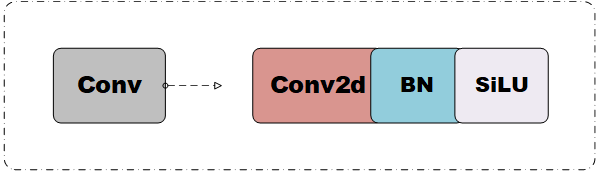
\includegraphics[width=0.67\linewidth]{chap2/CBS.png}
	\caption{\ \ 目标检测网络中的 $CBS$ 复合模块}
	\label{fig2-1}
\end{figure}
\vspace{3mm}

包含一个卷积层 Conv2d、一个 batchnormalization 层 BatchNorm2d 和一个 SiLU 激活函数层,为表示方便,我们直接将此 CBS 模块用 Conv 表示,
在基础模块中利用 SiLU 替换了原有的 LeakyReLU,是因为 SiLU 具有自稳定特性,SiLU 函数就是 Sigmoid 加权线性组合,其在负值的变化不再为零,从而抑制了大数量权重的学习。

第二个是 C3 模块,如图所示, 也是一个卷积复合模块,其是原有的 CSP 模块的替换,其核心思想还是局部跨阶段网络,一部分特征通过 CBS 模块提取特征,
另一部分通过 CBS 和 BottleNeck 模块处理,再与前者拼接进行卷积,而后输出,
\vspace{6mm}
\begin{figure}[h]
	\centering
	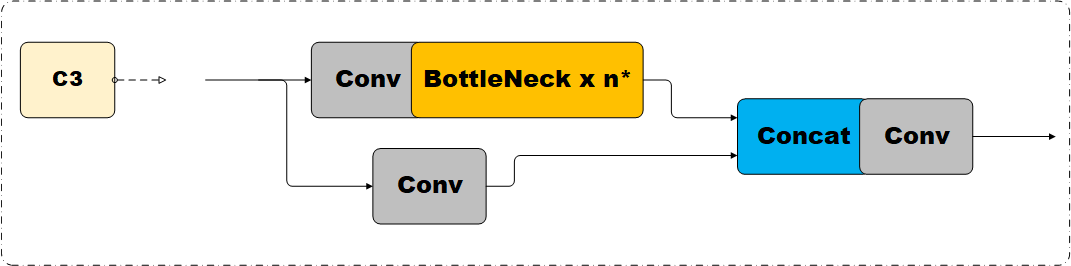
\includegraphics[width=0.67\linewidth]{chap2/C3.png}
	\caption{\ \ 目标检测网络中的 $C3$ 复合模块}
	\label{fig2-2}
\end{figure}
\vspace{3mm}
\vspace{6mm}
\begin{figure}[h]
	\centering
	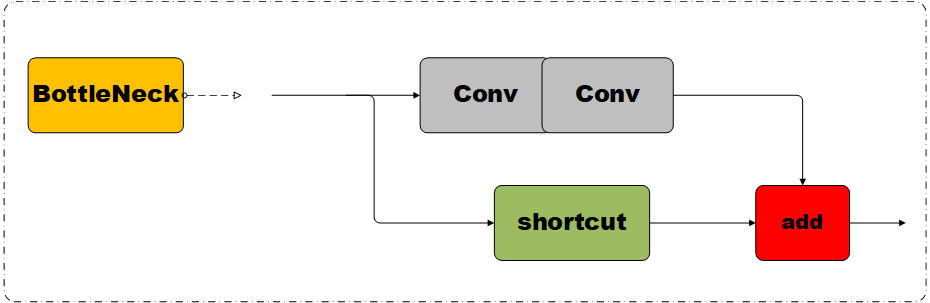
\includegraphics[width=0.67\linewidth]{chap2/Bottleneck.png}
	\caption{\ \ 目标检测网络中的 $BottleNeck$ 复合模块}
	\label{fig2-3}
\end{figure}
\vspace{3mm}
其中的 BottleNeck 模块是通过 shortcut 路径保留局部特征,并提取深层语义信息,将二者融合的一种方式,最后的改变点是 SPPF 模块,其是 PPF 的改进,与 PPF 具有相同的多尺度池化意义,新的架构中将 SPPF 换到了 backbone 的最后一层,
\vspace{6mm}
\begin{figure}[h]
	\centering
	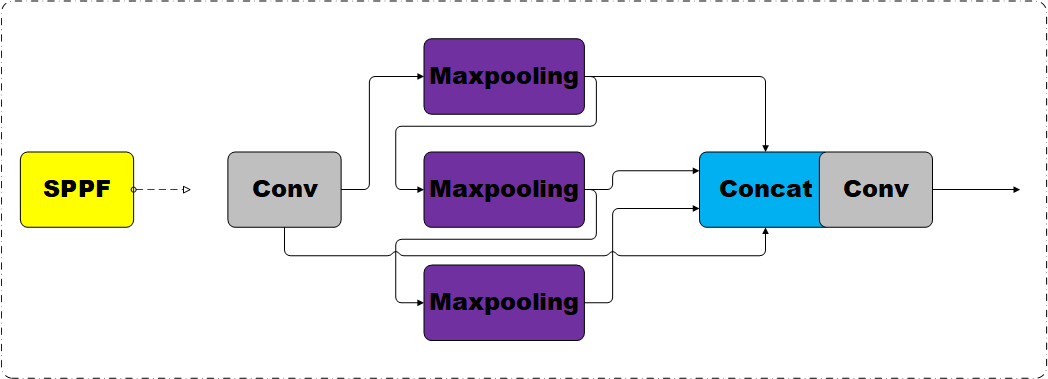
\includegraphics[width=0.67\linewidth]{chap2/SPPF.png}
	\caption{\ \ 目标检测网络中的 $SPPF$ 复合模块}
	\label{fig2-4}
\end{figure}
\vspace{3mm}
SPPF将每一层卷积后的池化效果复用,进一步池化,从而获得更多不同尺度特征,最终融合所有尺度特征,包含局部特征和全局特征,且速度上更快,所需浮点运算数更少,使得整个网络的架构更加简单。
另外,在输出层中,依旧沿用 FPN \+ PAN 的手段集合不同尺度特征,获得更加好的特征提取效果。
如图所示【YOLOv5】是整个检测网络架构,其具备更加简化的物理结构和更加优秀的检测精度,且提取三个不同尺度的特征进行检测,高度融合语义信息和空间信息,从而达到了一个近乎完美的检测精度,
在图中也可以看到其网络架构的简单性,这对于我们的算法应用意义也是不言而喻的。
且在最新的YOLOv5 6.0版本中有五种不同的量级网络,包括 n、s、m、l、x,其中 n 为最轻量级网络架构,也是我们工作的基石,而 x 是最大量级的网络架构,其余量级依次递增,
支持 tensorflow 和 keras 模型的导出,且同时支持 OpenCV dnn 和 onnx runtime 等,
总的来说,YOLOv5 6.0 的可移植性大大增强,而我们利用深度图像本身数据就少的特征,也是可以很好的进一步减少计算参数。

在有了这些基础模块后,就可以搭建整个多目标检测网络了,如图所示,是整个 YOLOv5 的网络模型框架,
可以看到,YOLOv5 的整个检测网络框架还是很高效的,是一种简单易移植的单阶段目标检测神经网络架构,
而且可以很直观的看到 YOLOv5 采取了三个不同尺度的输出特征进行最终的目标推理预测,符合多个尺度大小的目标检测标准,是对检测情景具有普适性的目标检测网络。

\vspace{6mm}
\begin{figure}[h]
	\centering
	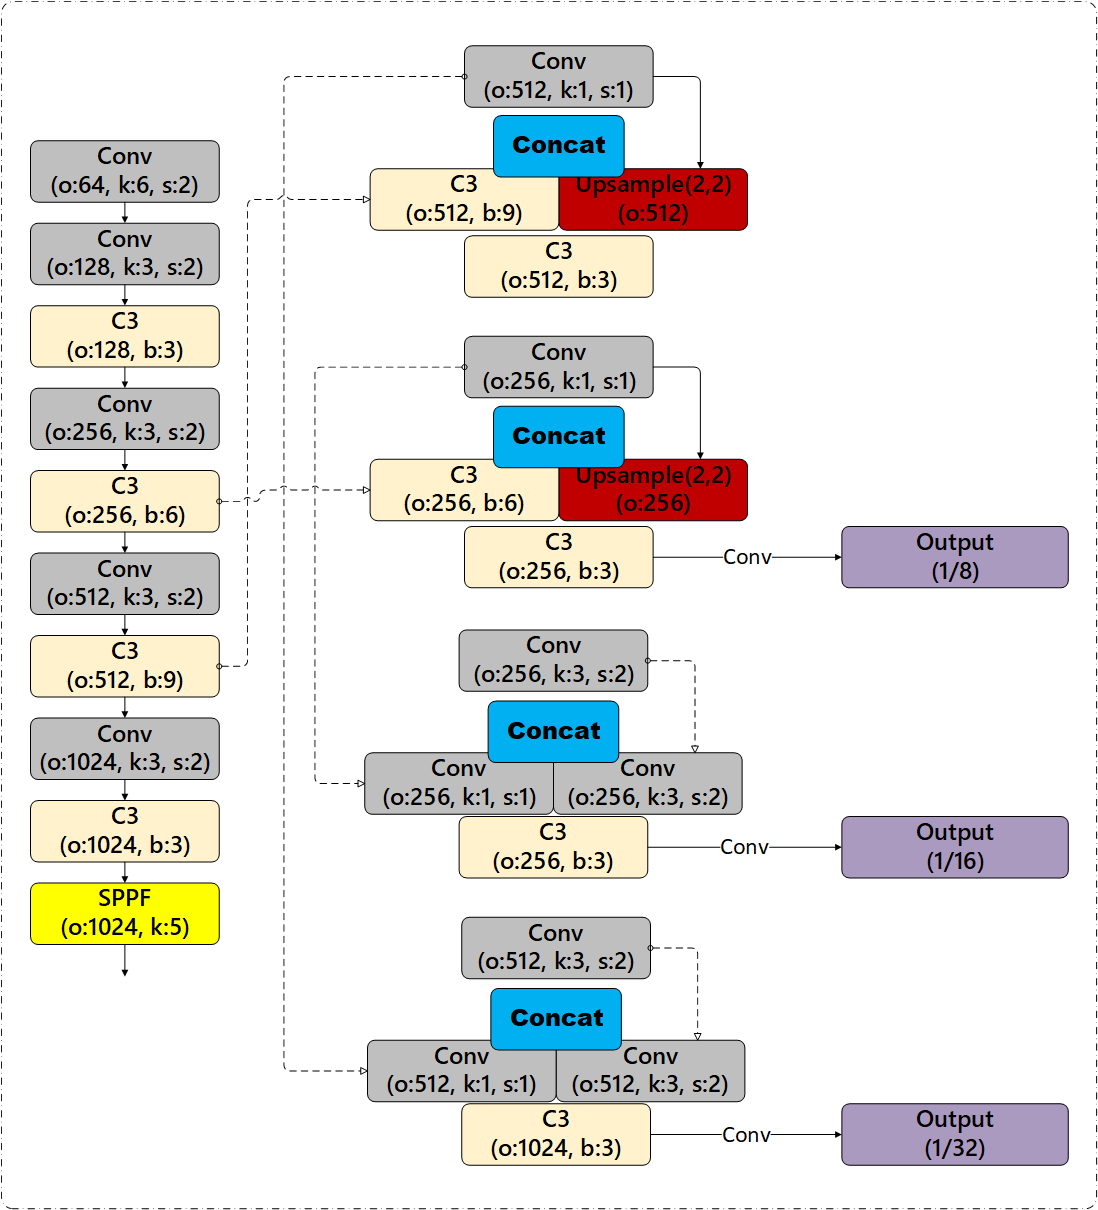
\includegraphics[width=0.67\linewidth]{chap2/YOLOv5.png}
	\caption{\ \ $YOLOv5\ \ 6.0$ 网络整体框架}
	\label{fig2-5}
\end{figure}
\vspace{3mm}

\section{实验}
\label{sec2-4}
这一部分首先介绍实验环境和实验结果指标,然后在五个不同数据集上使用我们提出的基于深度图像的多目标检测卷积神经网络进行测试并展示结果,以证明该网络的泛化性。

\subsection{实验环境}
PC配置为:Intel(R) Core(TM) i7-9700 CPU @ 3.00GHz * 8、48.0GB内存、GeForce GTX 1080 Ti GPU,GPU单元3584个,
系统为64位Ubuntu 18.04.6 LTS,CUDA版本为10.2.89、cuDNN版本为7.6.5,所有实验皆在Pytorch框架下完成。

\vspace{6mm}
\begin{figure}[h]
	\centering
	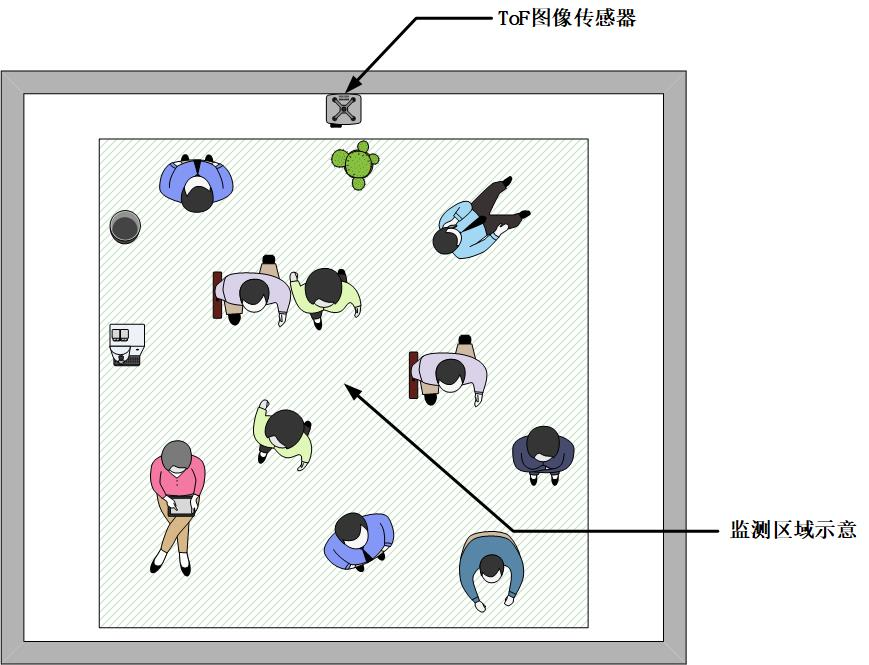
\includegraphics[width=0.67\linewidth]{chap2/surveillance.jpg}
	\caption{\ \ 多目标实时监测系统示意图}
	\label{fig2-6}
\end{figure}
\vspace{3mm}
如图是我们实验过程中的相机摆放方式和使用场景,其中深度图像传感器置于室内中央的顶部,垂直于地面进行拍摄。

\subsection{实验结果}
在我们的多目标检测网络实验中,我们使用前文提到的五个不同的数据集来进行测试该检测网络的鲁棒性,在所有检测结果中都达到了几乎一致的均值平均精度,值得注意的是对于不同数据集需要进行预训练过程。
在实验过程中,对检测结果的估量指标主要采用 mAP@0.5值、精确率 precision、召回率 recall、以及 F1 曲线,包含基础的 TPR、FPR、TNR、RNR,其中:

\begin{itemize}
	\item TPR(True Positive Rate): 实际为正例,预测为正例的概率;

	\item FPR(False Positive Rate): 实际为负例,预测为正例的概率;

	\item TNR(True Negative Rate): 实际为负例,预测为负例的概率;
	
	\item FNR(False Negative Rate): 实际为正例,预测为负例的概率;

	\item 精确率 : $ precision\ =\frac{TPR}{TPR\ +\ FNR} $;

	\item 召回率 : $ recall\ =\frac{FPR}{FPR\ +\ TNR} $;
	
	\item F1曲线 : $ F1\ =\frac{2TP}{2TP\ +\ FP\ +\ FN} $.
\end{itemize}

\\ \hspace*{\fill} \\
\textbf{GOTPD}

GOTPD数据集是网络上公开的数据集,需要线上申请,此数据集针对于多人目标检测,恰好对应我们使用场景,
即顶部视角的深度图像,此数据集由 $Kinect$ 相机拍摄,且是网络上数据量最大的数据集,共包含超过 4 万多张图像,图像分辨率为$512\times 424$,
且含有多种不同情况变体,像是人体性别外形、服饰衣帽、人流走向、群体间遮挡等,甚至加入了椅子之类的物件来测试鲁棒性,可以让我们为验证算法普适性做出针对性实验。
\vspace{6mm}
\begin{figure}[h]
	\centering
	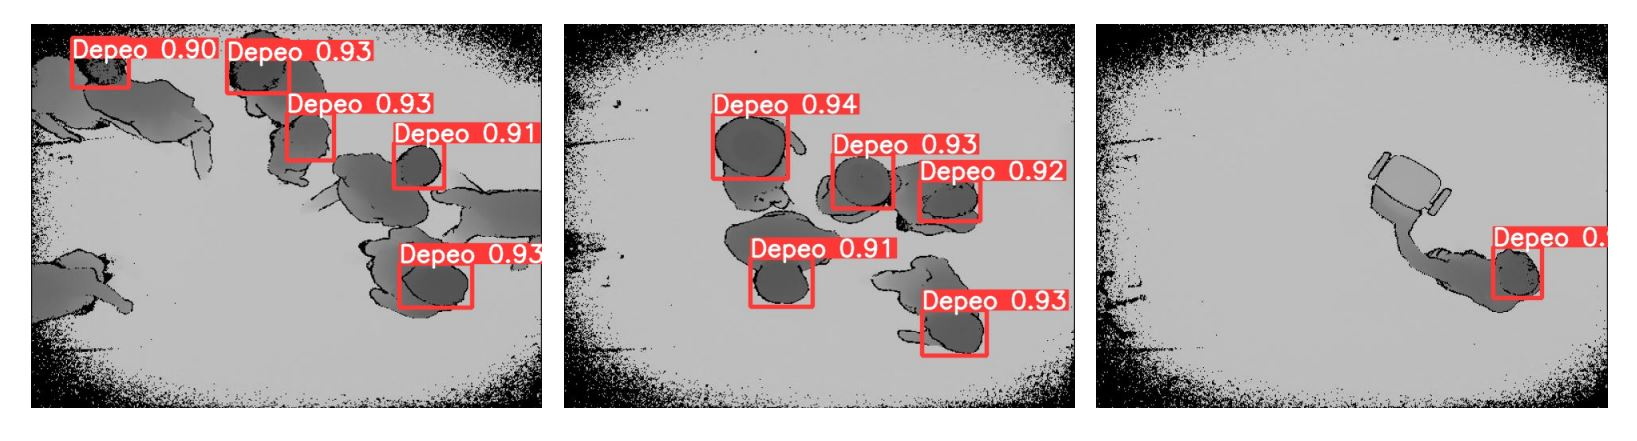
\includegraphics[width=0.67\linewidth]{chap2/GOTPD.jpg}
	\caption{\ \ 基于深度特征的多目标检测网络在 $GOTPD$ 数据集上检测结果}
	\label{fig2-7}
\end{figure}
\vspace{3mm}

\begin{figure}[htbp]
	\begin{minipage}{0.48\linewidth}
		\centering
		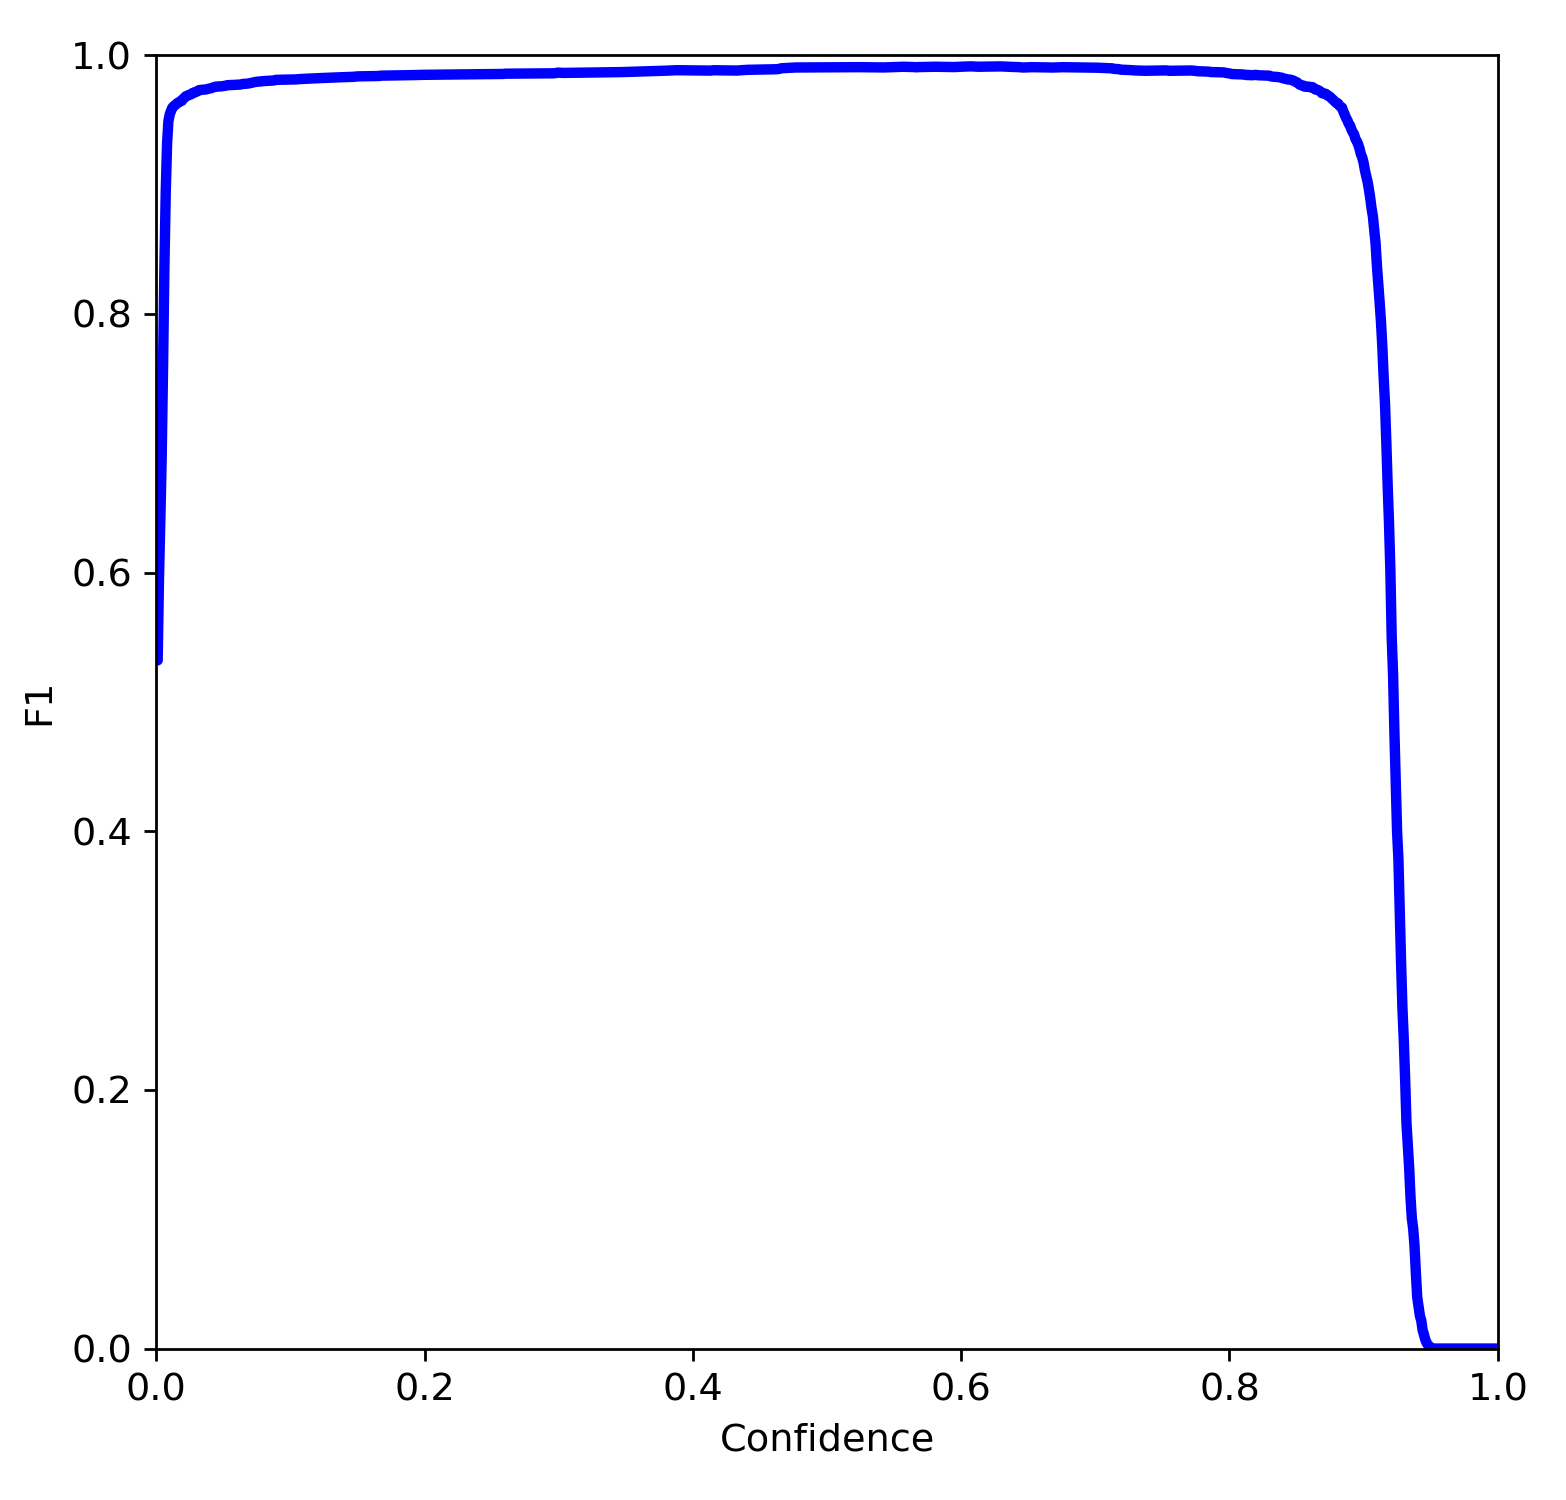
\includegraphics[width=0.9\linewidth]{chap2/GOTPDF1.png}
		\caption{\ \ 多目标检测网络在 $GOTPD$ 数据集上的 $F1$ 曲线}
		\label{fig2-8}%文中引用该图片代号
	\end{minipage}
	\begin{minipage}{0.48\linewidth}
		\centering
		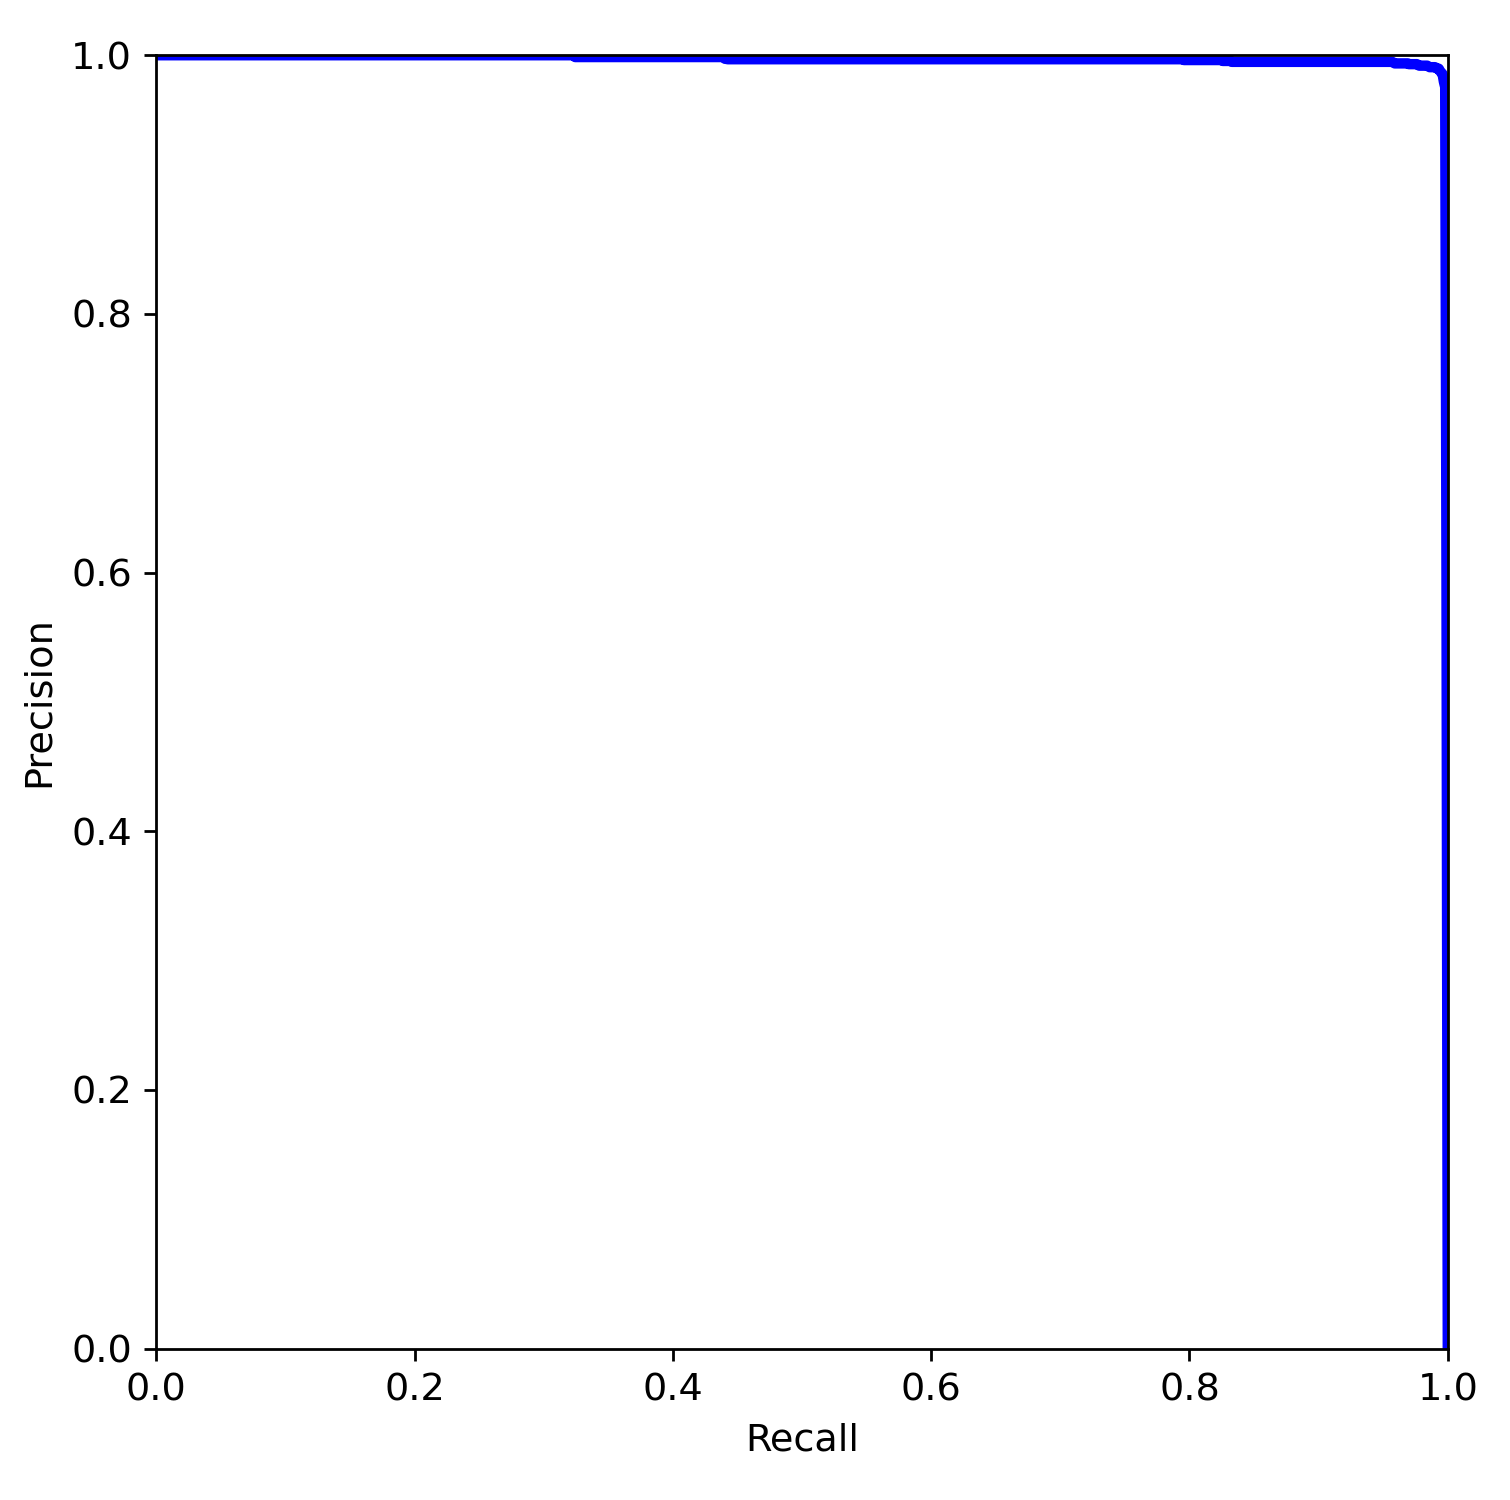
\includegraphics[width=0.9\linewidth]{chap2/GOTPDPR.png}
		\caption{\ \ 多目标检测网络在 $GOTPD$ 数据集上的 $PR$ 曲线}
		\label{fig2-9}%文中引用该图片代号
	\end{minipage}
\end{figure}

如图是检测网络在此数据集上的一些多目标检测结果。
而后分别是其 F1 曲线和 PR 曲线,精确率和召回率都达到了高水平的 1.00,且 mAP@0.5 值即均值平均精度达到了 0.993 的水准,对于一个实时检测系统来说已经是很好的水平了。

\\ \hspace*{\fill} \\
\textbf{ToFC}
	
ToFC数据集也是在网络上寻找到的公开数据集,此数据集是二进制文件格式,需自己单独编写脚本解码处理获得深度图像,此数据集的分辨率仅有$320\times 240$,相对较低,
但保留了完整深度图像数据,是我们针对低分辨率数据做测试的选择。
\vspace{6mm}
\begin{figure}[htbp]
	\centering
	\begin{minipage}{0.48\linewidth}
		\centering
		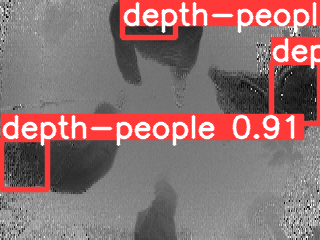
\includegraphics[width=1.0\linewidth]{chap2/TOFC1.png}
		\caption{\ \ 基于深度特征的多目标检测网络在 $TOFC$ 数据集上检测结果1}
		\label{fig2-10}%文中引用该图片代号
	\end{minipage}
	\begin{minipage}{0.48\linewidth}
		\centering
		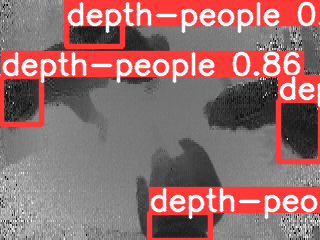
\includegraphics[width=1.0\linewidth]{chap2/TOFC2.png}
		\caption{\ \ 基于深度特征的多目标检测网络在 $TOFC$ 数据集上检测结果2}
		\label{fig2-11}%文中引用该图片代号
	\end{minipage}
\end{figure}

如图是检测网络在 ToFC 数据集上的一些多目标检测结果。

\begin{figure}[htbp]
	\begin{minipage}{0.48\linewidth}
		\centering
		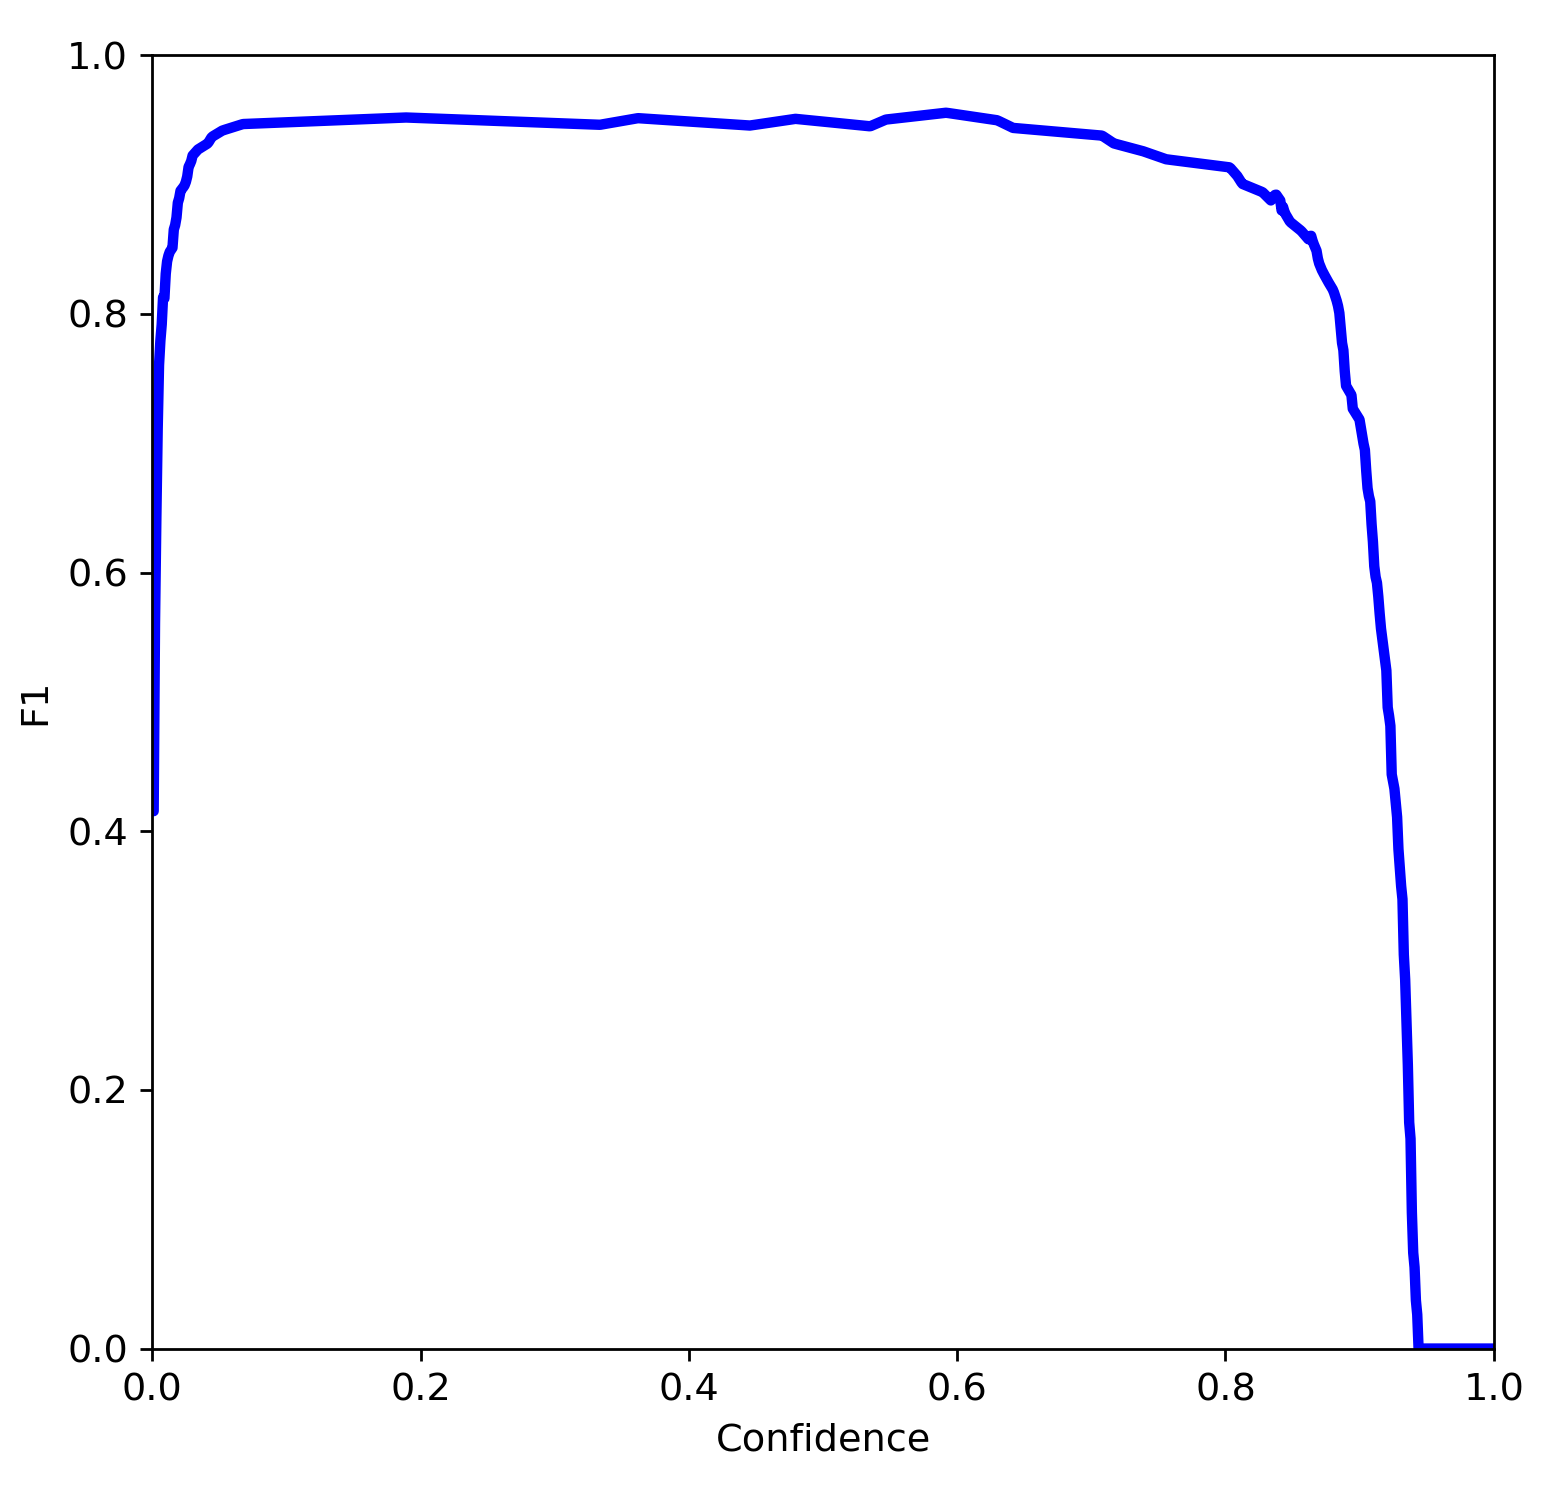
\includegraphics[width=0.9\linewidth]{chap2/TOFCF1.png}
		\caption{\ \ 多目标检测网络在 $TOFC$ 数据集上的 $F1$ 曲线}
		\label{fig2-12}%文中引用该图片代号
	\end{minipage}
	\begin{minipage}{0.48\linewidth}
		\centering
		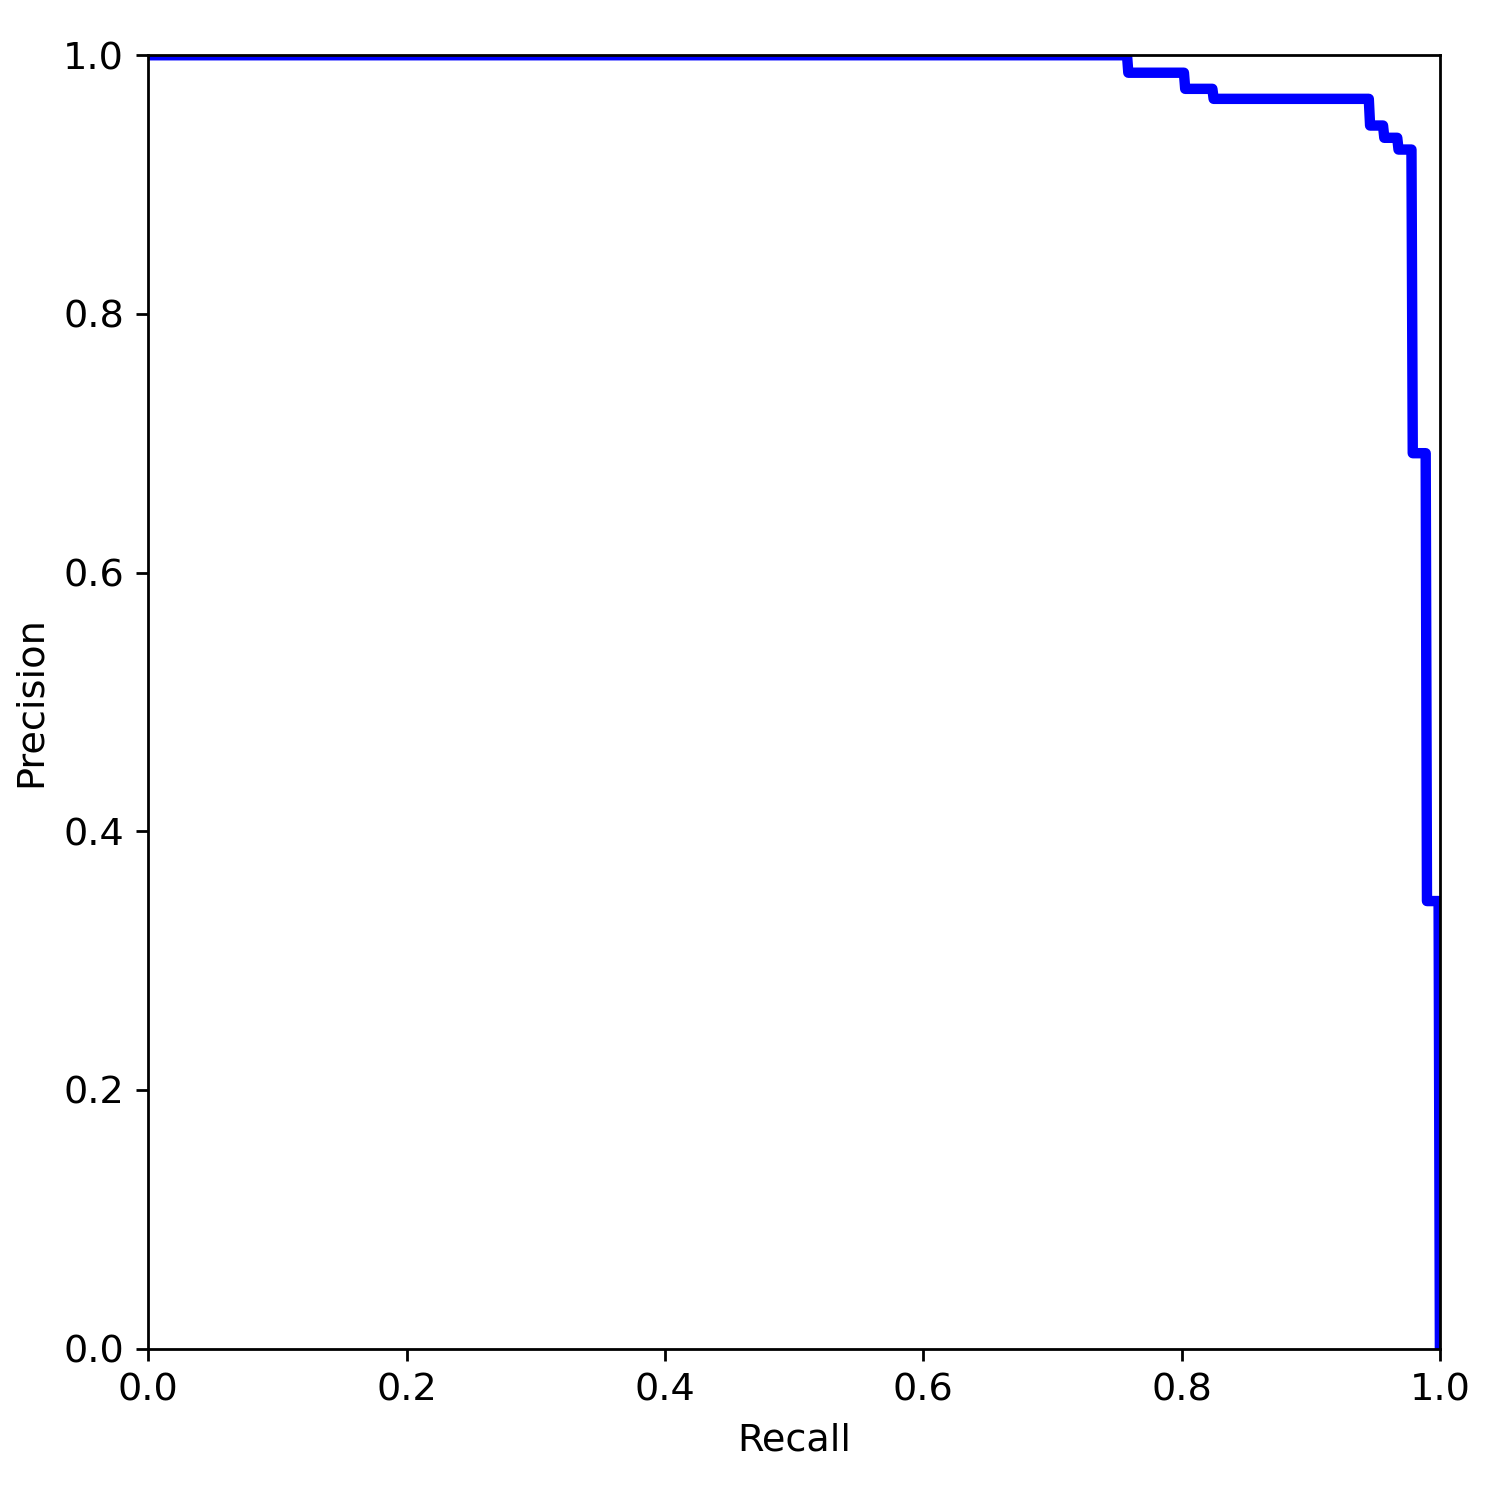
\includegraphics[width=0.9\linewidth]{chap2/TOFCPR.png}
		\caption{\ \ 多目标检测网络在 $TOFC$ 数据集上的 $PR$ 曲线}
		\label{fig2-13}%文中引用该图片代号
	\end{minipage}
\end{figure}
\vspace{3mm}

以上是其 F1 曲线和 PR 曲线,该检测网络在 TOFC 数据集上的表现稍有逊色,其均值平均精度只达到了 0.978 的水平,这与该数据集的低分辨率也有部分关系,
分辨率的降低意味着不同点之间的高度变化不再那么精确,但其精确率和召回率仍然达到了 1.00。

\\ \hspace*{\fill} \\
\textbf{Axon}
	
此数据集为实验室单独拍摄,所使用相机为 Axon M3M,是一款以ToF图像传感器为基础的微型图像传感器,其分辨率可以达到$640\times 480$,包括单张图像和视频录制,
这也是我们实验过程中最轻便的一款图像传感器,极大地方便部署硬件设施到天花板上,此数据集我们采集了一千多张训练数据,并得到很好的测试效果。
\begin{figure}[htbp]
	\centering
	\begin{minipage}{0.48\linewidth}
		\centering
		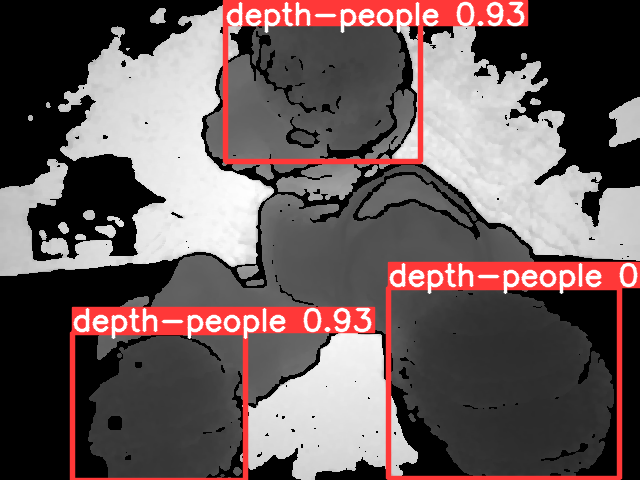
\includegraphics[width=1.0\linewidth]{chap2/Axon1.png}
		\caption{\ \ 基于深度特征的多目标检测网络在 $Axon$ 数据集上检测结果1}
		\label{fig2-14}%文中引用该图片代号
	\end{minipage}
	\begin{minipage}{0.48\linewidth}
		\centering
		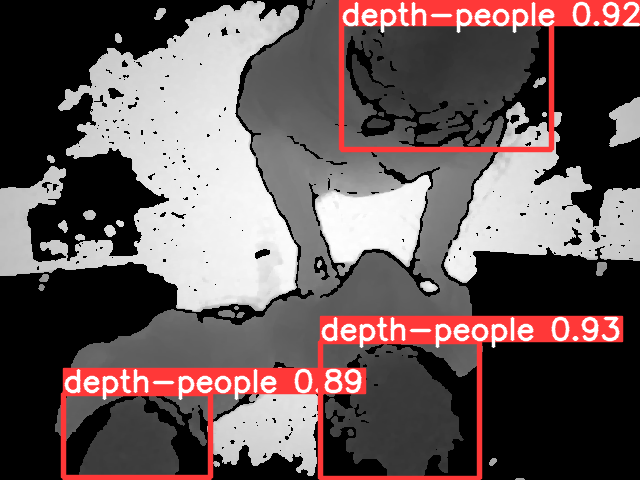
\includegraphics[width=1.0\linewidth]{chap2/Axon2.png}
		\caption{\ \ 基于深度特征的多目标检测网络在 $Axon$ 数据集上检测结果2}
		\label{fig2-15}%文中引用该图片代号
	\end{minipage}
\end{figure}

如图是检测网络在 Axon 数据集上的一些多目标检测结果。
随后分别是 F1 和 PR 曲线,也可以看到 Axon 数据集上仍然达到了 1.00 的精确率和召回率,且 mAP@0.5 值达到了 0.994 的最高水平,这也是本次实验中最轻量级的图像传感器。
\begin{figure}[htbp]
	\begin{minipage}{0.48\linewidth}
		\centering
		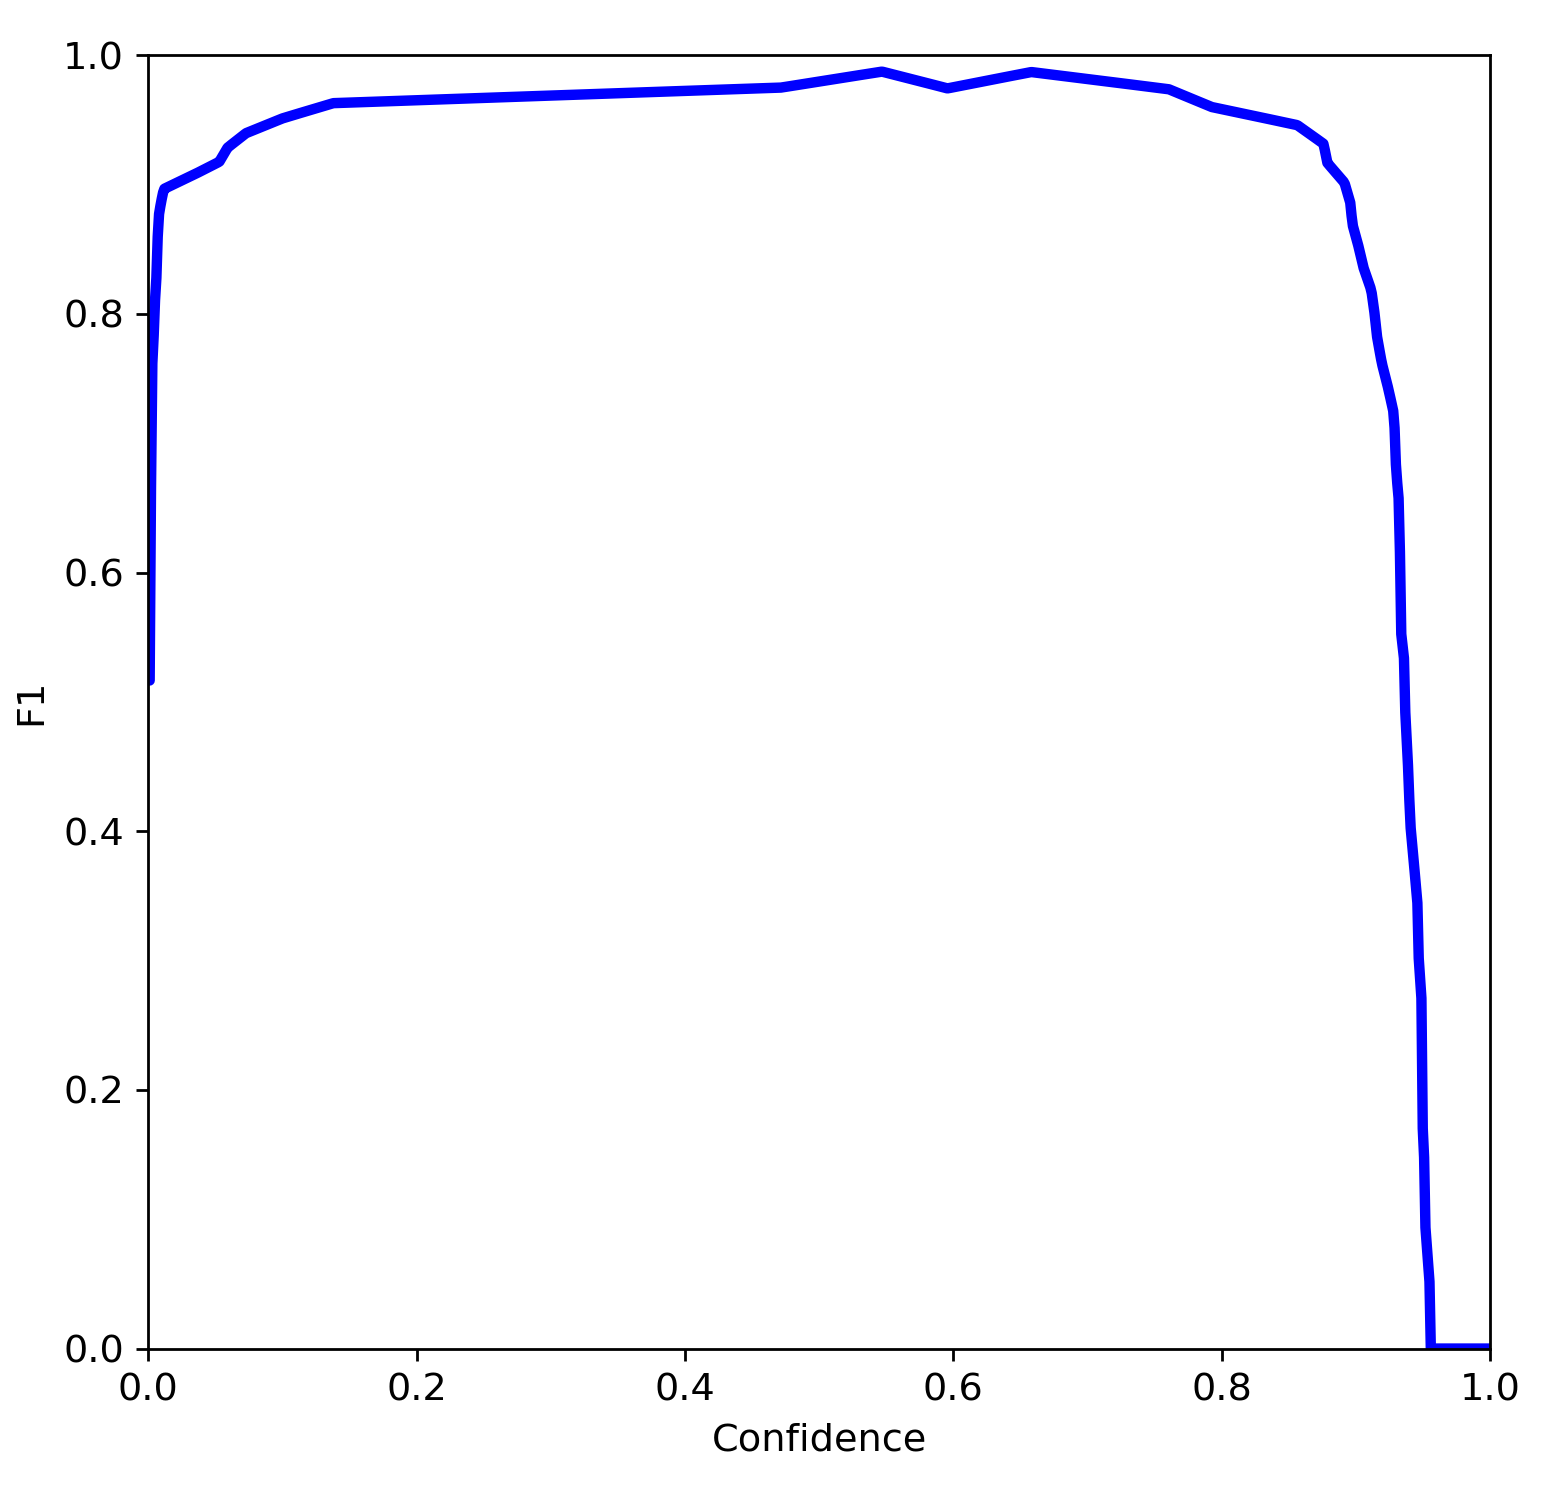
\includegraphics[width=0.9\linewidth]{chap2/AxonF1.png}
		\caption{\ \ 多目标检测网络在 $Axon$ 数据集上的 $F1$ 曲线}
		\label{fig2-16}%文中引用该图片代号
	\end{minipage}
	\begin{minipage}{0.48\linewidth}
		\centering
		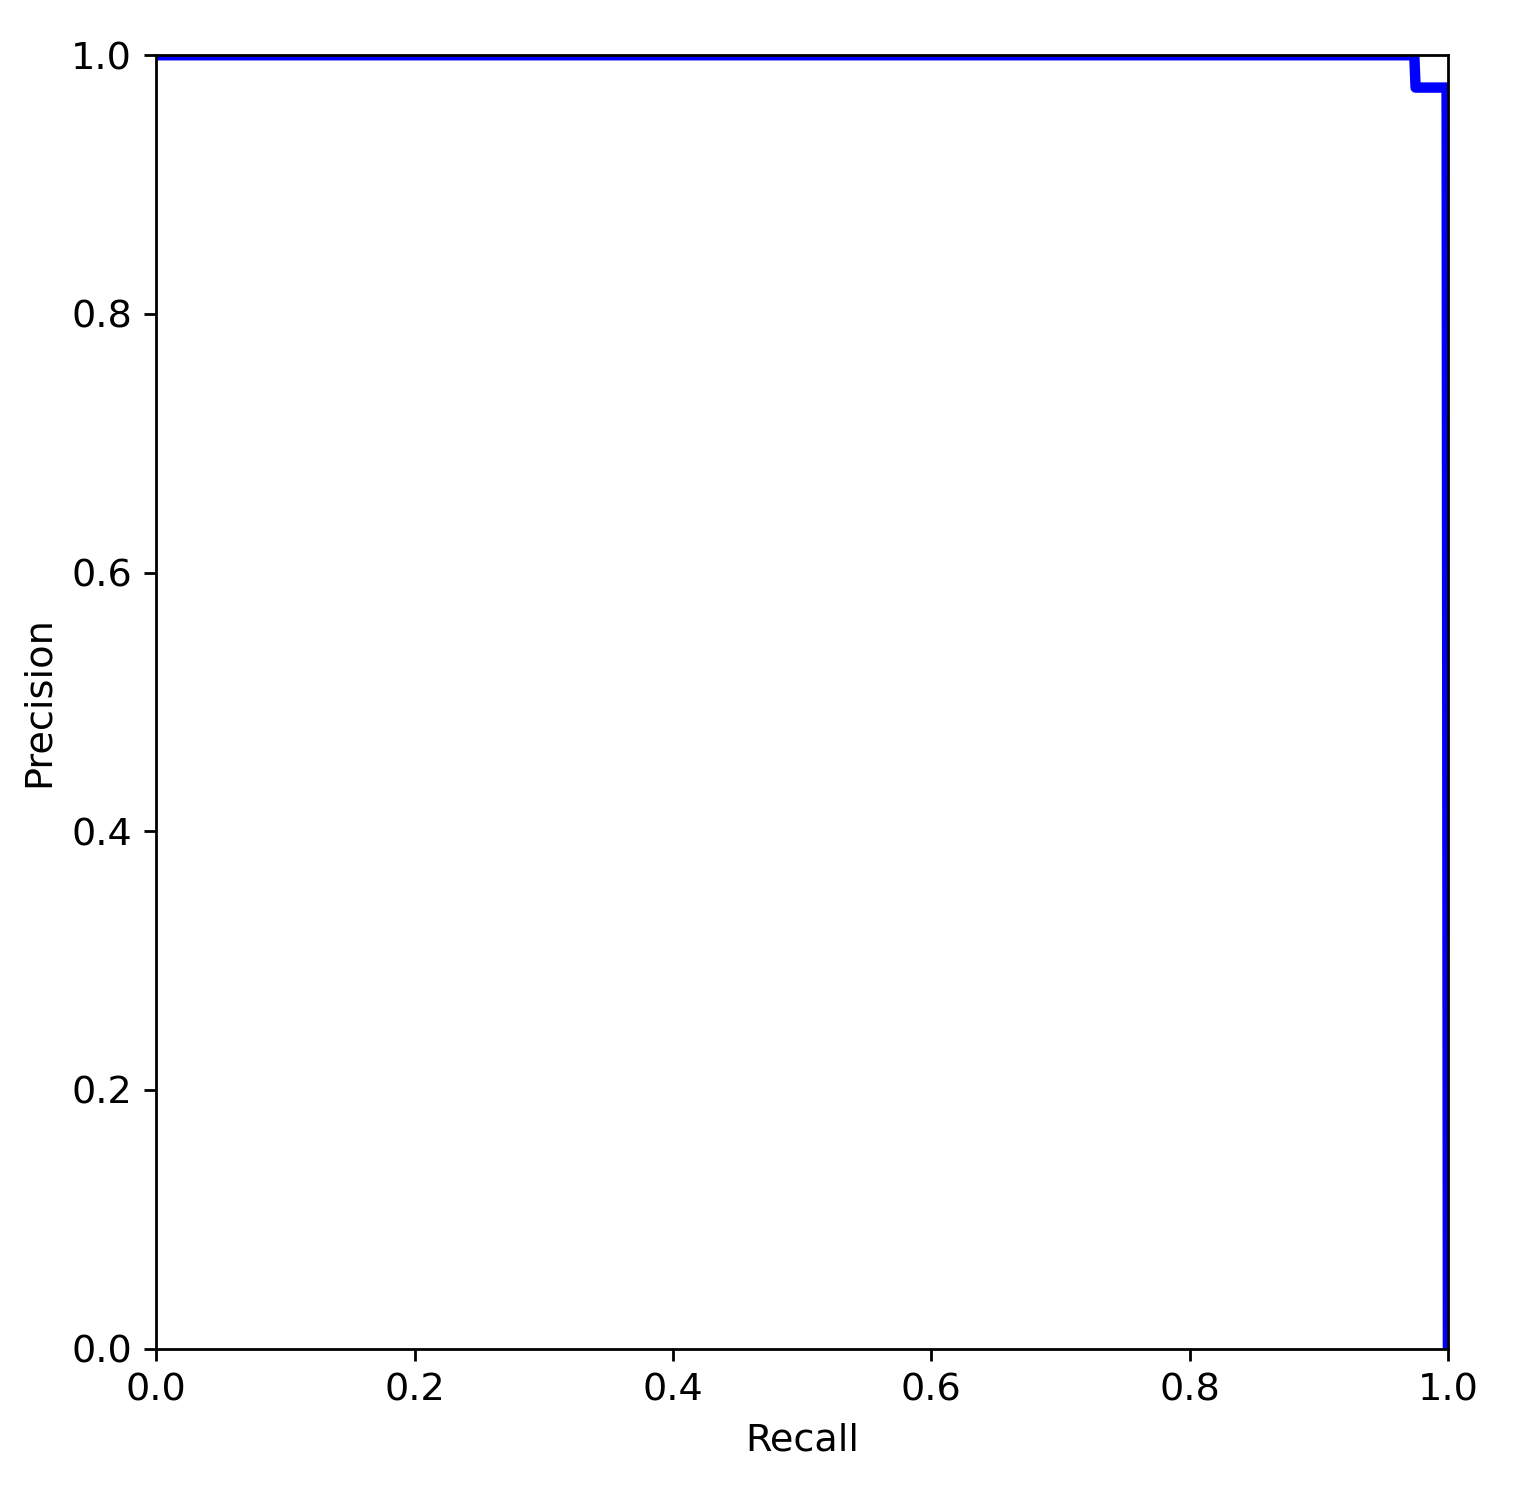
\includegraphics[width=0.9\linewidth]{chap2/AxonPR.png}
		\caption{\ \ 多目标检测网络在 $Axon$ 数据集上的 $PR$ 曲线}
		\label{fig2-17}%文中引用该图片代号
	\end{minipage}
\end{figure}

\\ \hspace*{\fill} \\
\textbf{Kinect v2}

此数据集亦为实验室单独拍摄,所使用相机为 Kinect v2,是一款 Microsoft 推出的高性能的多功能相机,包含 RGB、红外图像等,但我们只采集其中的深度图像,其水平 FOV 为70°,垂直 FOV 为60°,
分辨率可达$512\times 424$,与普遍 ToF 传感器的参数相同,其实验结果能代表大多深度相机的结果。
\begin{figure}[htbp]
	\centering
	\begin{minipage}{0.48\linewidth}
		\centering
		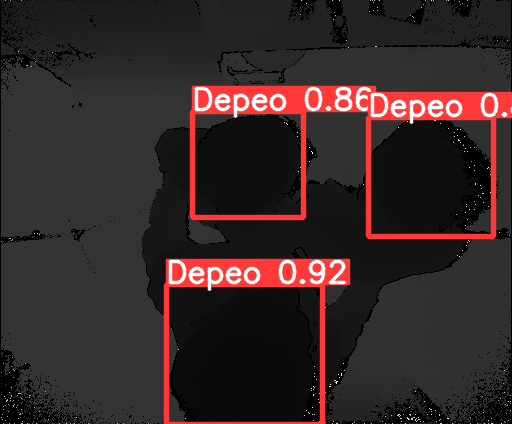
\includegraphics[width=1.0\linewidth]{chap2/v21.png}
		\caption{\ \ 基于深度特征的多目标检测网络在 $Kinect\ v2$ 数据集上检测结果1}
		\label{fig2-18}%文中引用该图片代号
	\end{minipage}
	\begin{minipage}{0.48\linewidth}
		\centering
		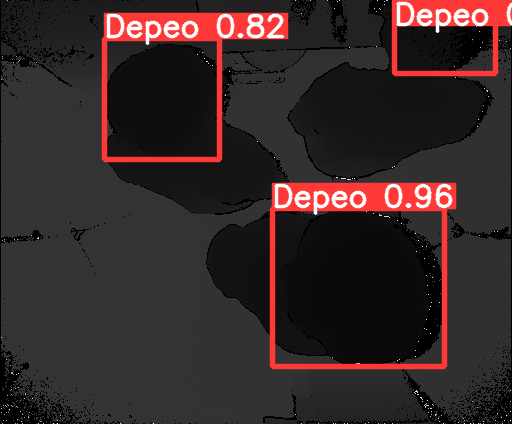
\includegraphics[width=1.0\linewidth]{chap2/v22.png}
		\caption{\ \ 基于深度特征的多目标检测网络在 $Kinect\ v2$ 数据集上检测结果2}
		\label{fig2-19}%文中引用该图片代号
	\end{minipage}
\end{figure}

如图是检测网络在此数据集上的一些多目标检测结果。
随后的是其 F1 曲线和 PR 曲线,在 v2 数据集上的检测结果也没有达到均值水平,其 mAP@0.5 值只能达到 0.982,其精确率和召回率仍然达到 1.00 水平,其分辨率也是较低,
但是适合实时应用的设置,也是我们实现整个实时监测系统时使用的图像传感器。
\begin{figure}[htbp]
	\begin{minipage}{0.48\linewidth}
		\centering
		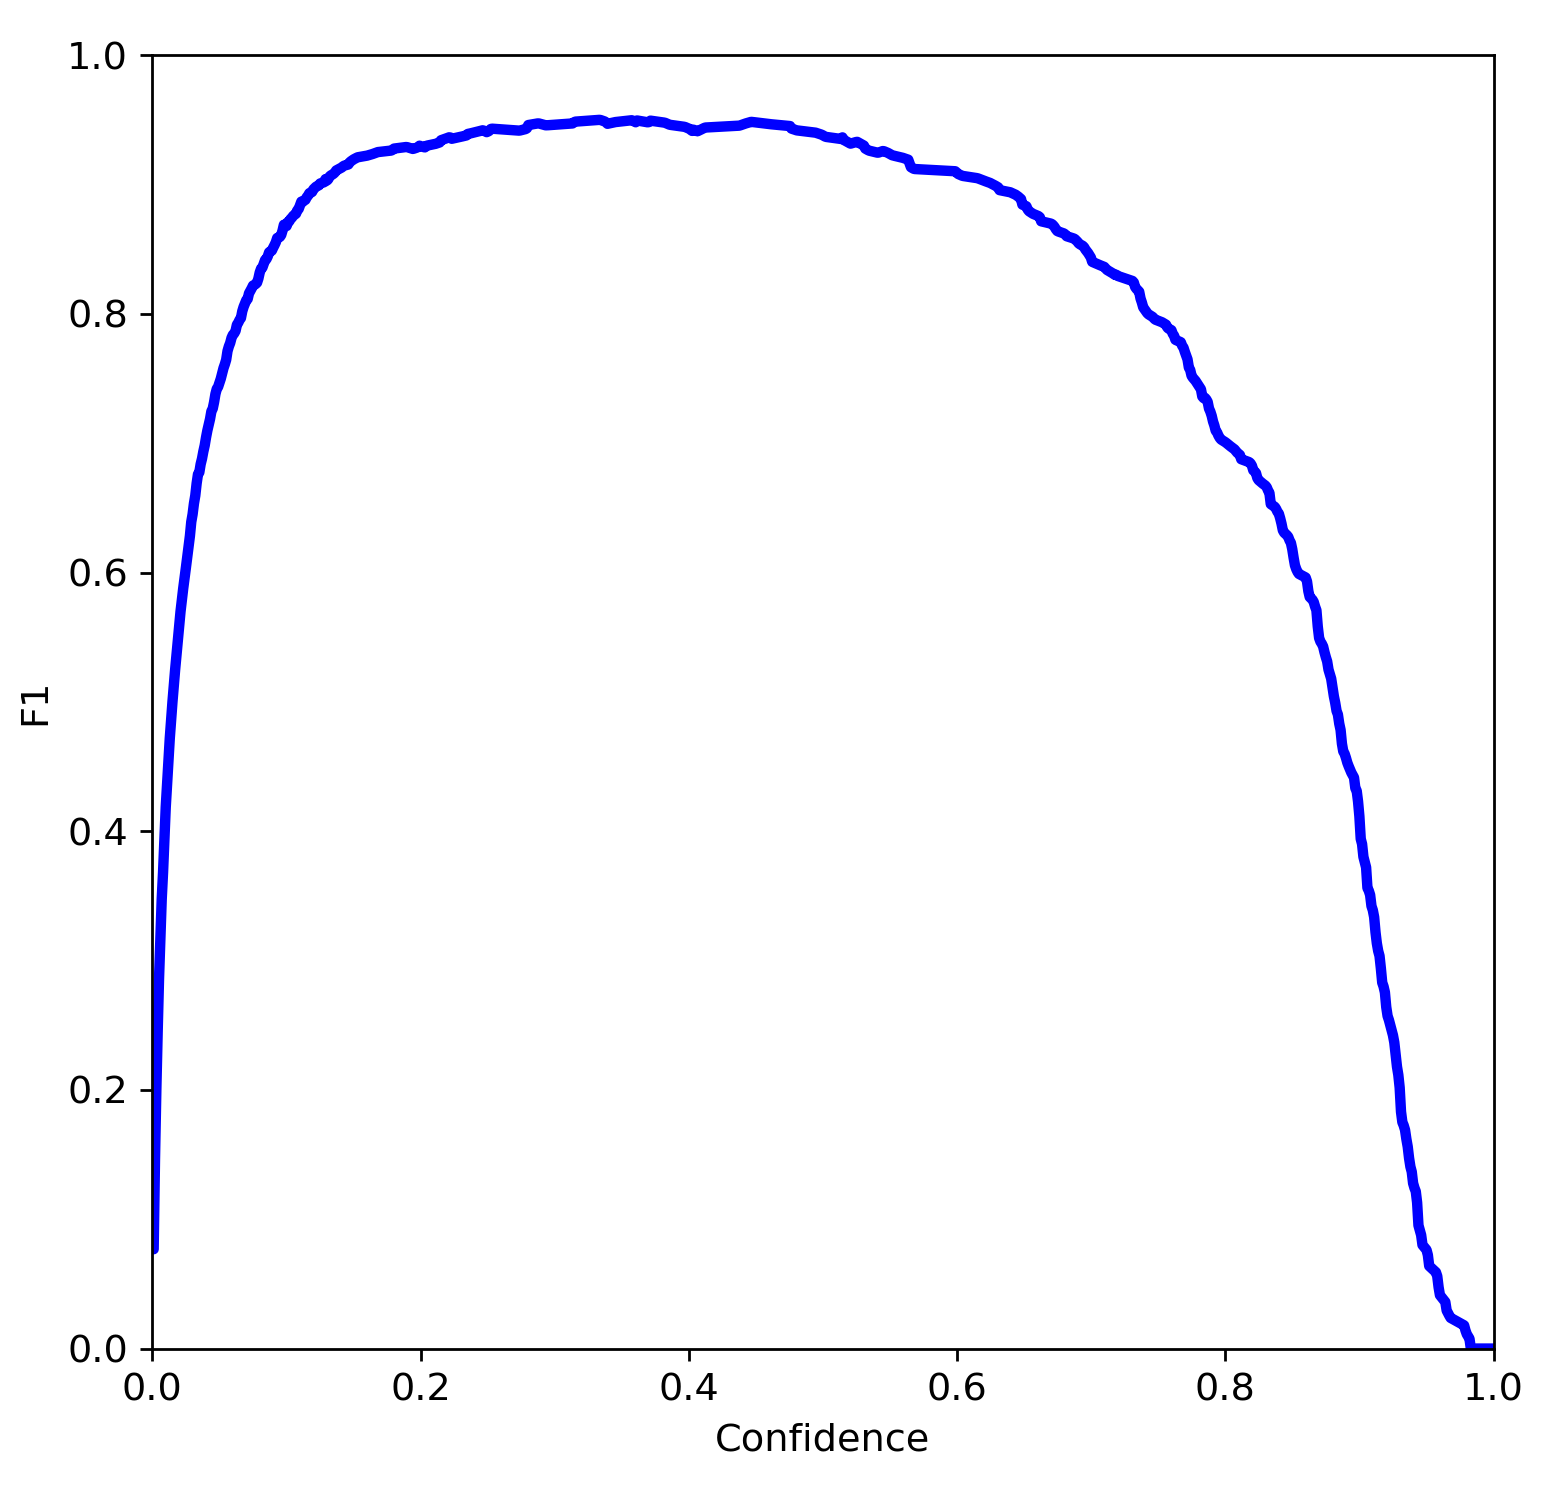
\includegraphics[width=0.9\linewidth]{chap2/v2F1.png}
		\caption{\ \ 多目标检测网络在 $Kinect\ v2$ 数据集上的 $F1$ 曲线}
		\label{fig2-20}%文中引用该图片代号
	\end{minipage}
	\begin{minipage}{0.48\linewidth}
		\centering
		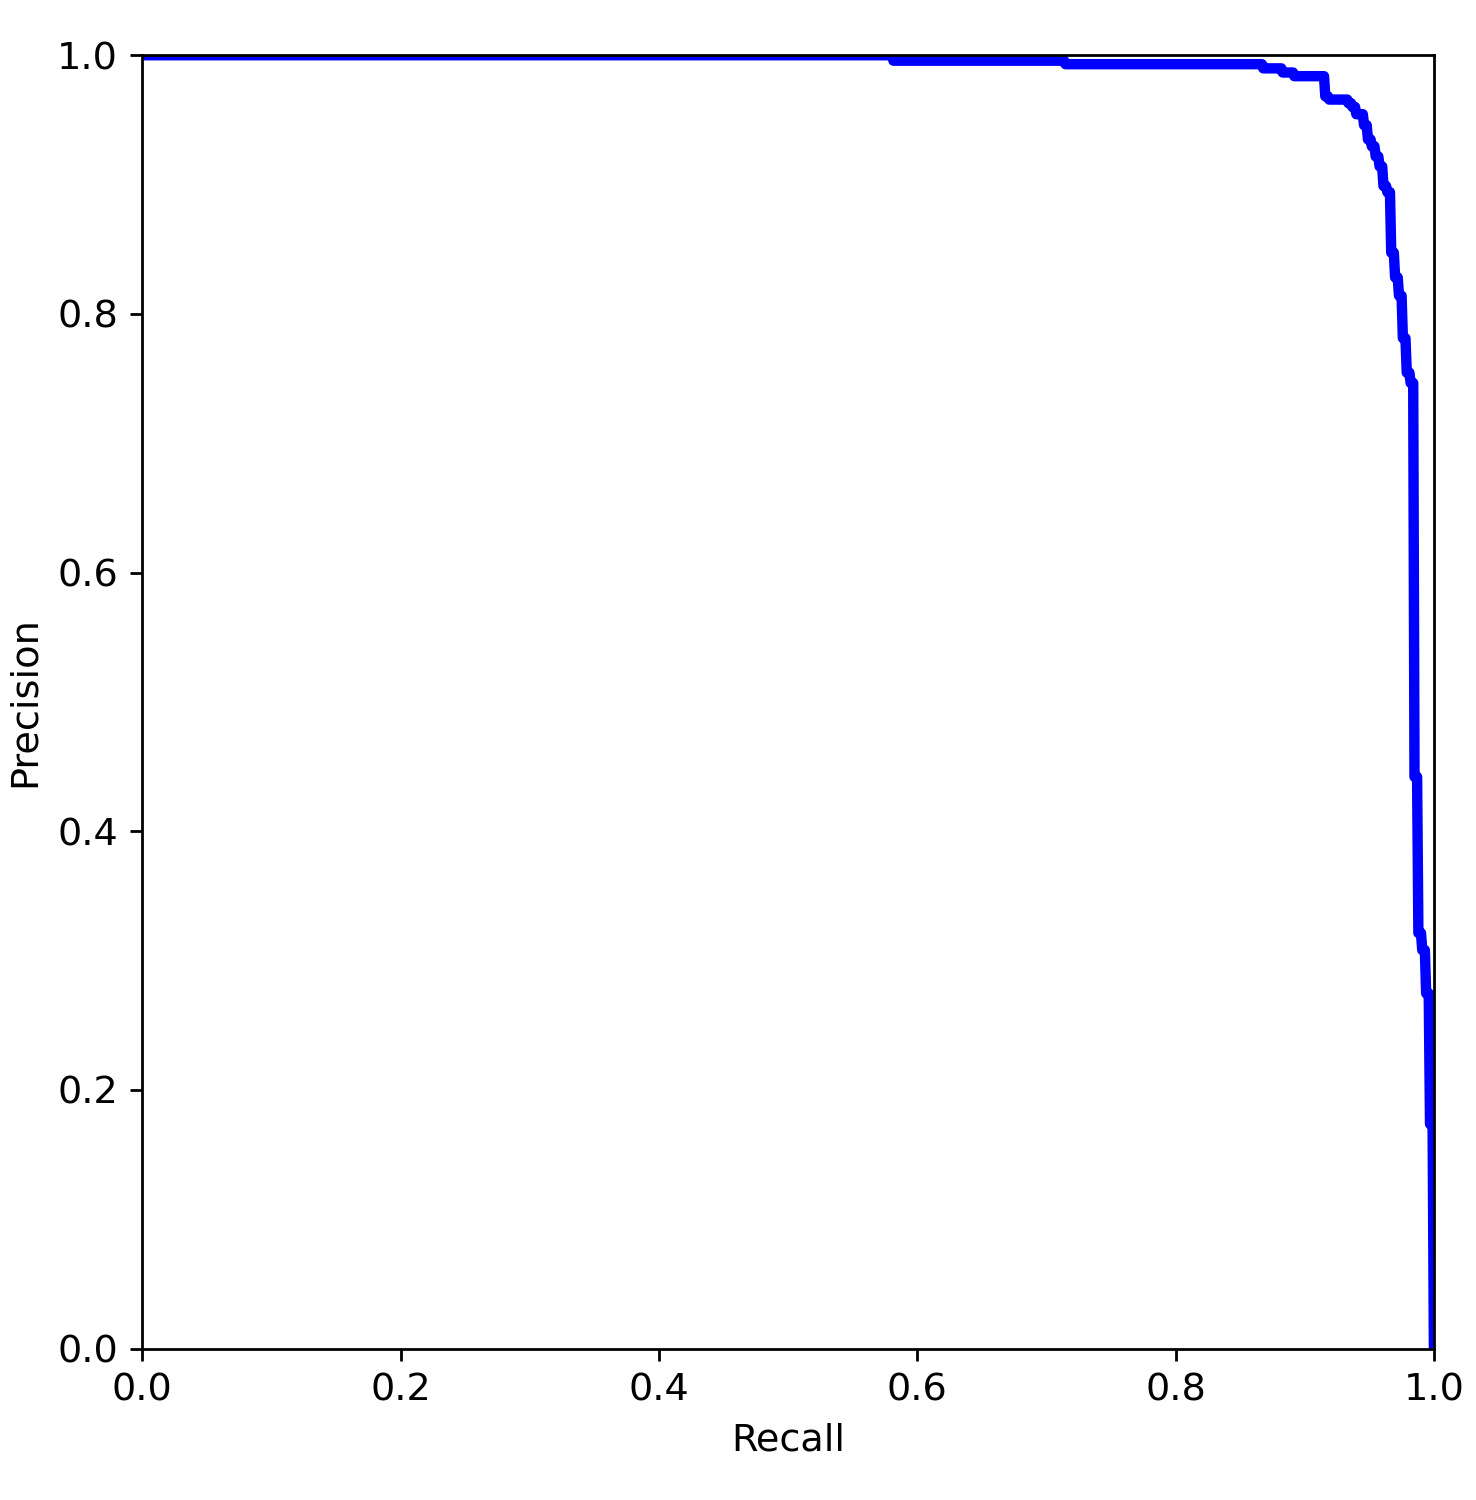
\includegraphics[width=0.9\linewidth]{chap2/v2PR.png}
		\caption{\ \ 多目标检测网络在 $Kinect\ v2$ 数据集上的 $PR$ 曲线}
		\label{fig2-21}%文中引用该图片代号
	\end{minipage}
\end{figure}

\\ \hspace*{\fill} \\
\textbf{Azure}

\begin{figure}[htbp]
	\centering
	\begin{minipage}{0.48\linewidth}
		\centering
		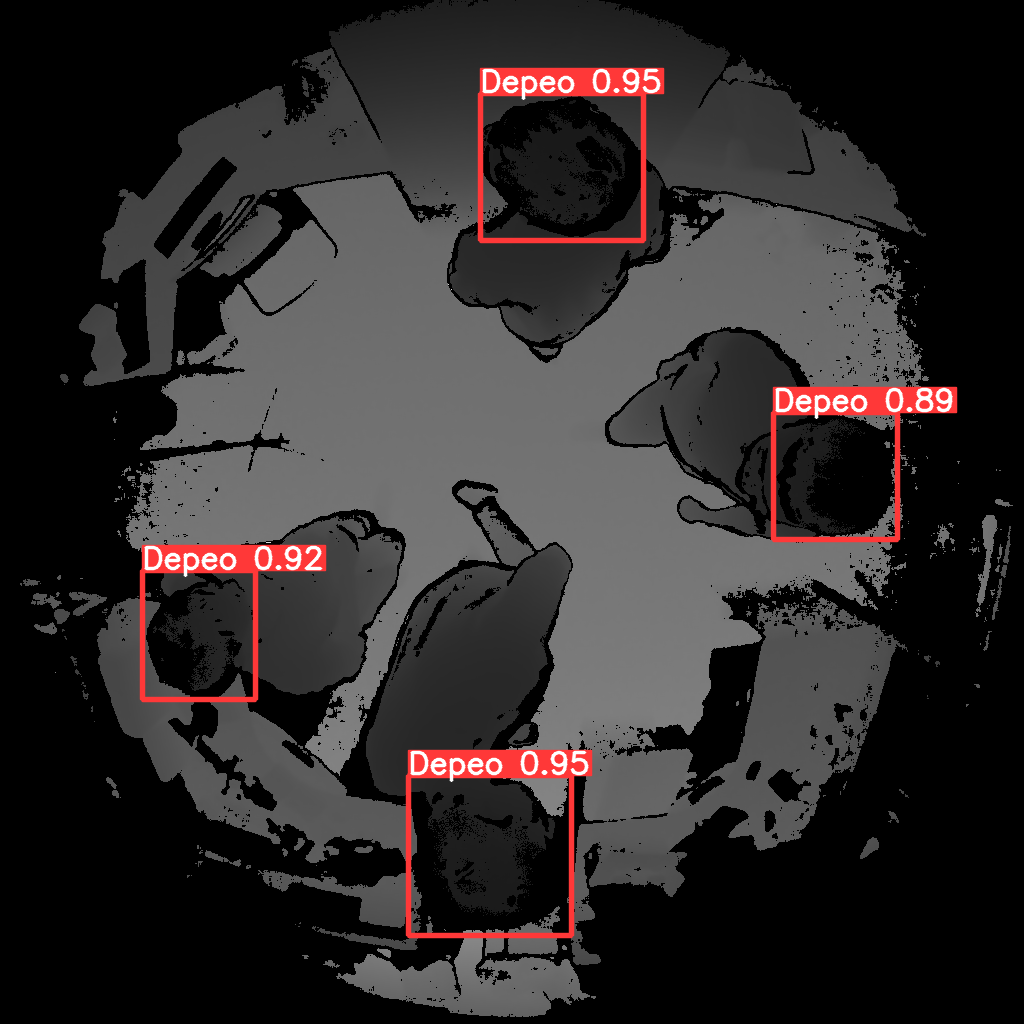
\includegraphics[width=1.0\linewidth]{chap2/v41.png}
		\caption{\ \ 基于深度特征的多目标检测网络在 $Azure$ 数据集上检测结果1}
		\label{fig2-22}%文中引用该图片代号
	\end{minipage}
	\begin{minipage}{0.48\linewidth}
		\centering
		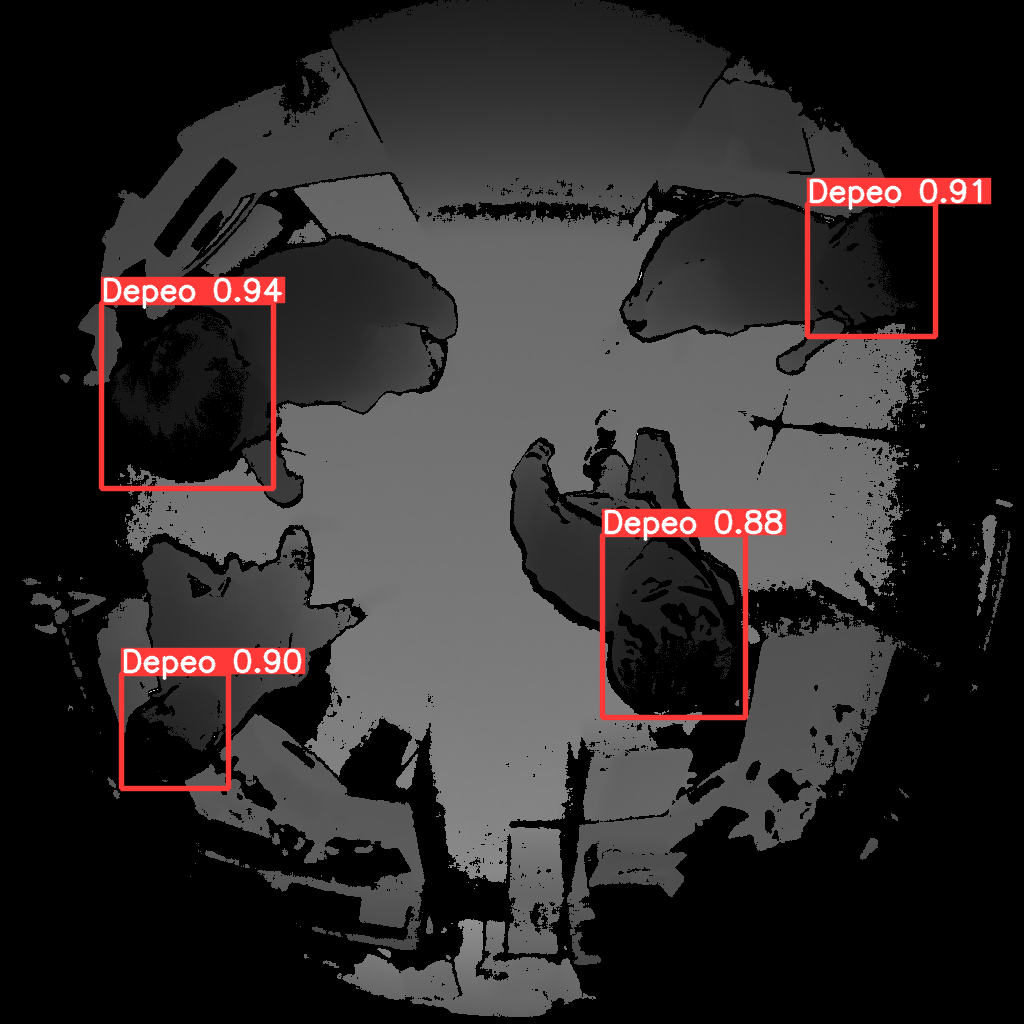
\includegraphics[width=1.0\linewidth]{chap2/v42.png}
		\caption{\ \ 基于深度特征的多目标检测网络在 $Azure$ 数据集上检测结果2}
		\label{fig2-23}%文中引用该图片代号
	\end{minipage}
\end{figure}

此数据集亦为实验室单独拍摄,所使用相机为Azure Kinect,也是一款 Microsoft 推出的高性能的多功能相机,同样包含RGB、深度图像等,其深度图像广角模式最高分辨率可达$1024\times 1024$,
对应 FOI 为 120° × 120°,普通模式分辨率可达$640\times 576$,对应 FOI 为 75° × 65°,是我们针对高分辨率数据做测试的选择。
此数据集分辨率最高,其 mAP@0.5 值即均值平均精度也达到了 0.993 的高水准,且含有 1.00 的精确率和召回率,在其 F1 和 PR 曲线也能看到训练过程的稳定性。
\begin{figure}[htbp]
	\begin{minipage}{0.48\linewidth}
		\centering
		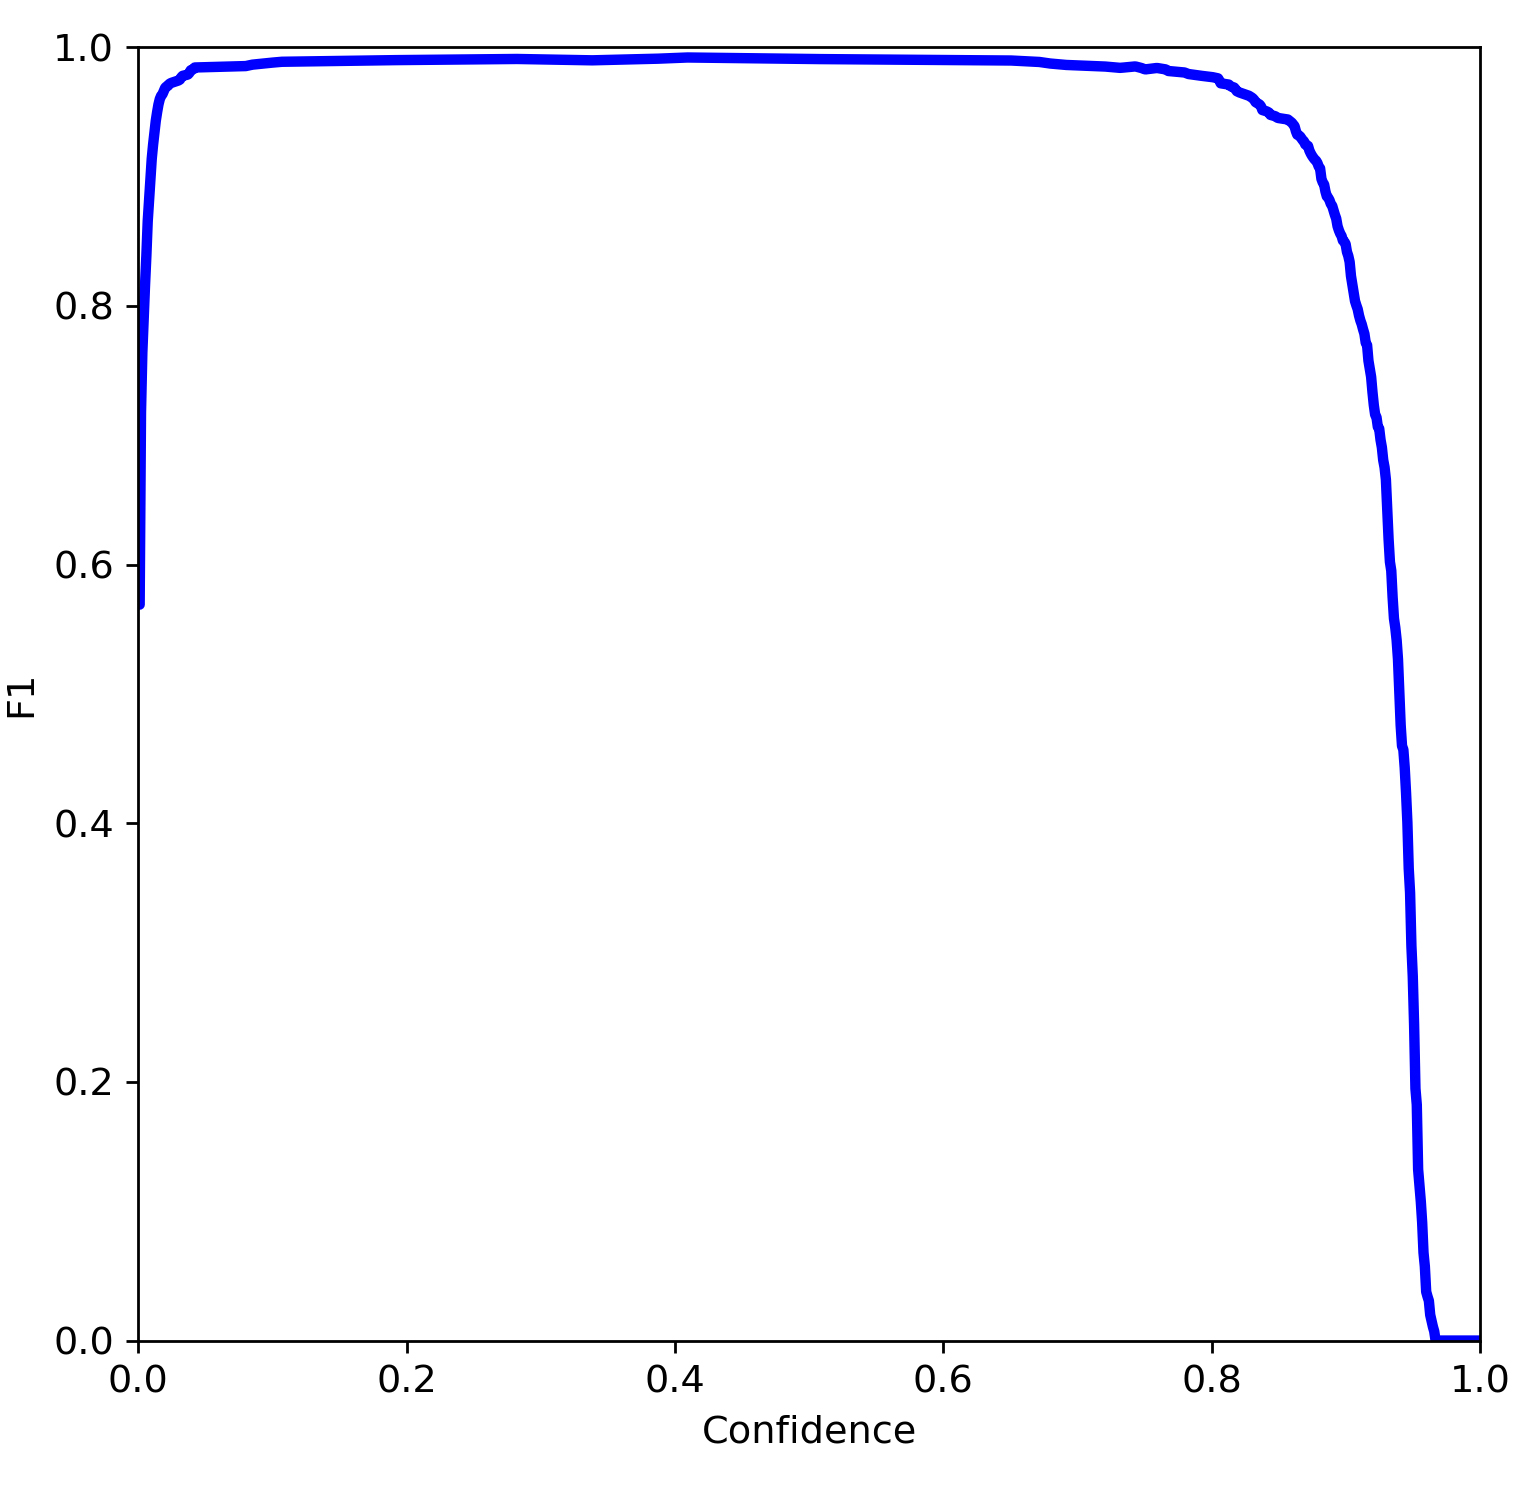
\includegraphics[width=0.9\linewidth]{chap2/v4F1.jpg}
		\caption{\ \ 多目标检测网络在 $Azure$ 数据集上的 $F1$ 曲线}
		\label{fig2-24}%文中引用该图片代号
	\end{minipage}
	\begin{minipage}{0.48\linewidth}
		\centering
		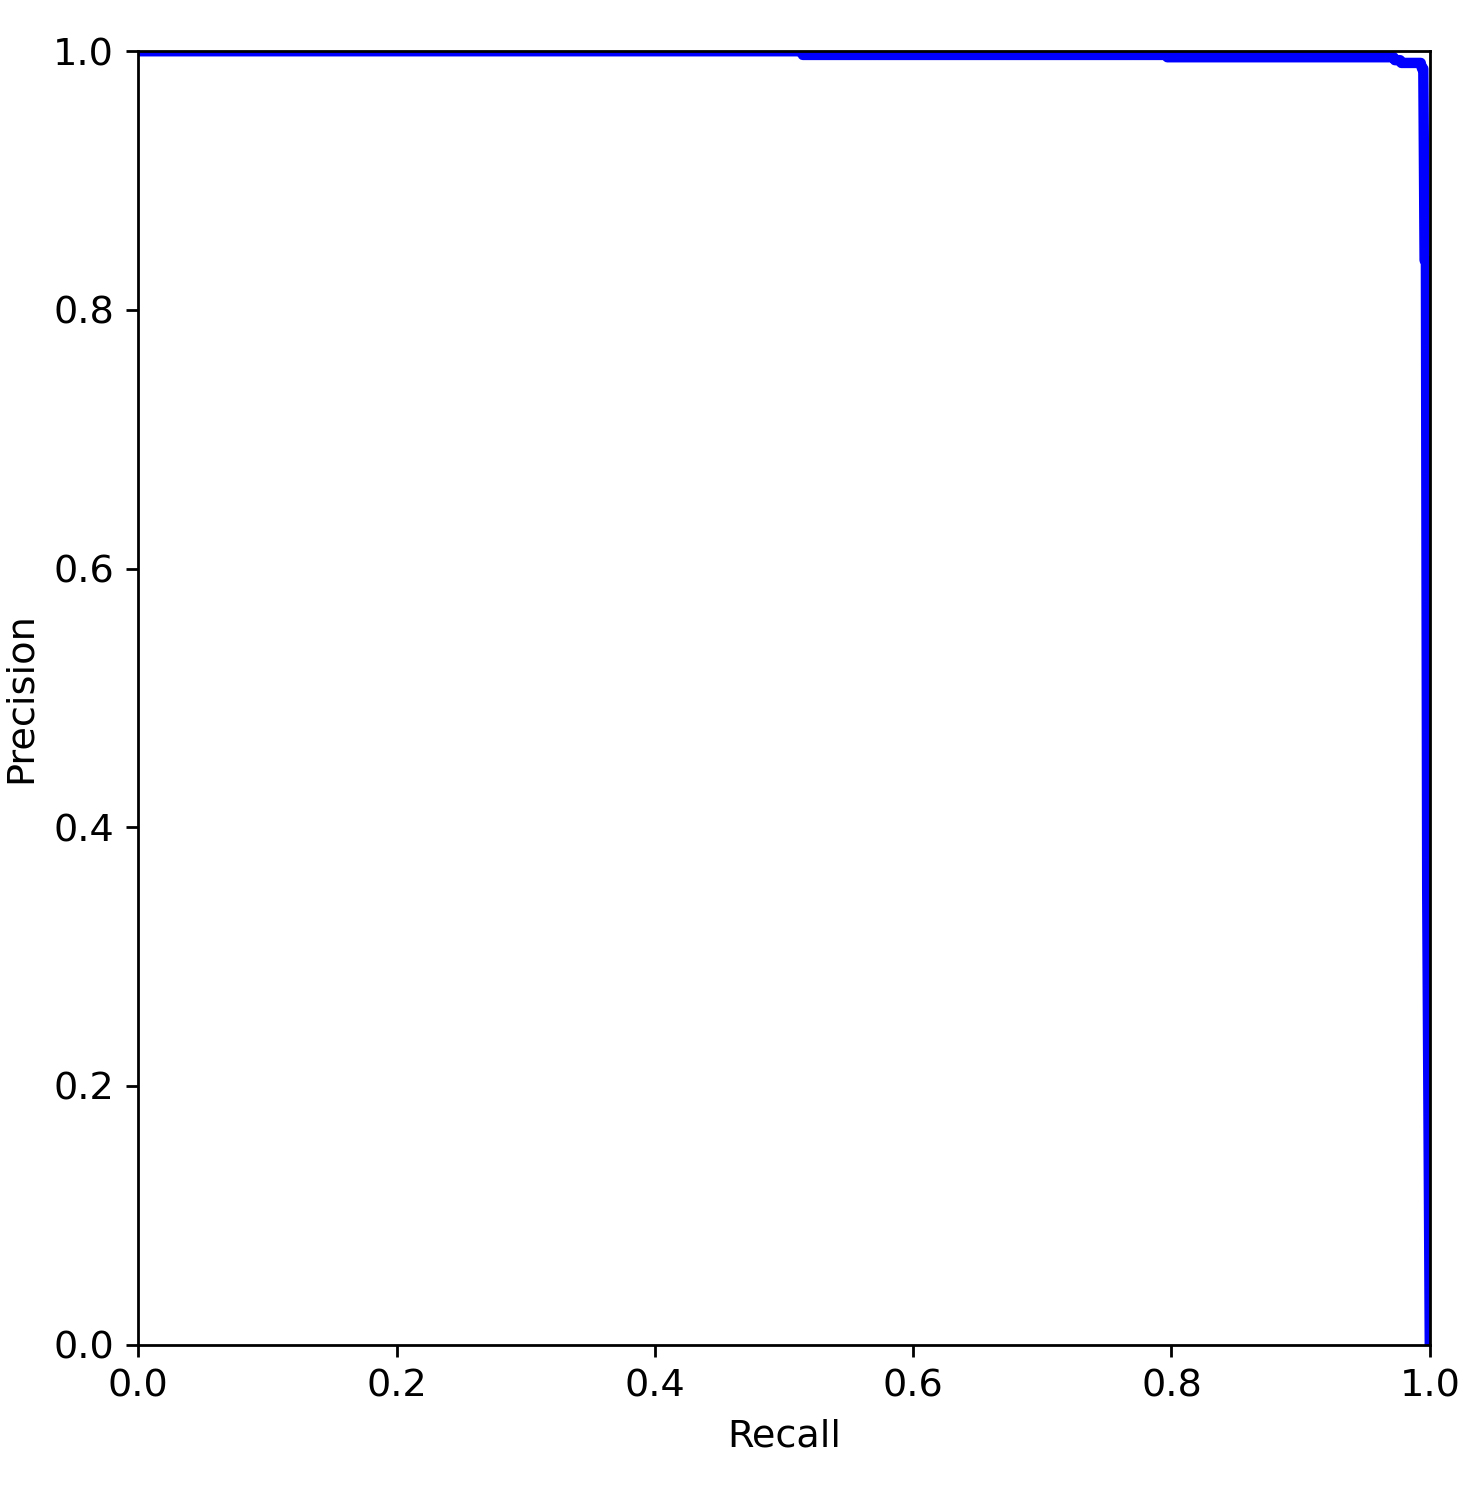
\includegraphics[width=0.9\linewidth]{chap2/v4PR.jpg}
		\caption{\ \ 多目标检测网络在 $Azure$ 数据集上的 $PR$ 曲线}
		\label{fig2-25}%文中引用该图片代号
	\end{minipage}
\end{figure}

\vspace{6mm}
\begin{figure}[h]
	\centering
	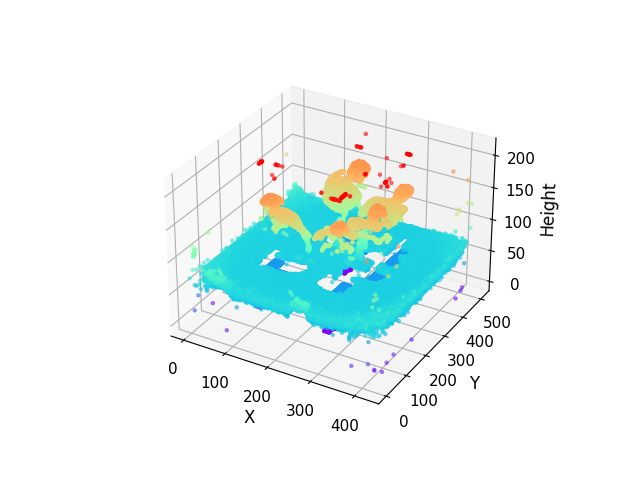
\includegraphics[width=0.67\linewidth]{chap2/GOTPDETEC.png}
	\caption{\ \ 检测神经网络在$GOTPD$数据集上的推理过程可视化结果}
	\label{fig2-26}
\end{figure}
\vspace{3mm}

除此之外,上图是我们在此网络推理过程中学习到的特征的展示,使用的是 GOTPD 数据集中的一帧图像,可以清楚地看到,此检测网络只需利用获取的深度特征就可以辨别出待追踪目标。

\subsection{与现有方法的比较}

表2 - 1比较了现有的大部分多目标检测神经网络的检测结果,对多个检测场景下的因素进行归纳分析,包括神经网络架构、图像来源、数据集、图像角度等。
从对比结果可以看出, YOLOv5 6.0 的检测结果还是相当鲁棒的,对于公开对比的 GOTPD 数据集和我们自行拍摄的 Axon、Kinect 数据集都有着很优秀的均值平均精度,取得了最好的性能指标,
且多个不同数据集测试也表明了其是具有普适性的检测网络,适合于在大多数场景下使用。

\begin{table} [htpb]
	\begin{center}
		%\setlength{\belowcaptionskip}{3mm}
		\caption{\ \ 不同多目标检测方法准确度对比}
		\label{table2-1}
		\footnotesize
		%\setlength{\tabcolsep}{1.8pt}
		\begin{tabular}{llrrrrrrr}
			\hline
			\multirow{1}*{Methods} & \multirow{1}*{Input Data} & \multirow{1}*{Dataset} & \multirow{1}*{View} & \multirow{1}*{TPR} & \multirow{1}*{FPR} & \multirow{1}*{mAP@0.5}\\
			\hline \hline
			%You Only Look Once
			Fast YOLO \cite{37} & RGB & VOC2007+2012 & sideview & - & - & 0.527\\
			YOLO \cite{37} & RGB & VOC2007+2012 & sideview & - & - & 0.664\\
			%YOLOv3 : An Incremental Improvement
			SSD513 \cite{40} & RGB & COCO & sideview & - & - & 0.504\\
			YOLOv3 \cite{40} & RGB & COCO & sideview & - & - & 0.579\\
			%SSD Single Shot MultiBox Detector 
			Faster R-CNN \cite{42} & RGB & VOC2007+2012 & sideview & - & - & 0.704\\
			SSD300 \cite{42} & RGB & VOC2007+2012 & sideview & - & - & 0.724\\
			SSD512 \cite{42} & RGB & VOC2007+2012 & sideview & - & - & 0.749\\
			Faster R-CNN \cite{42} & RGB & VOC2007+2012+COCO & sideview & - & - & 0.759\\
			SSD300 \cite{42} & RGB & VOC2007+2012+COCO & sideview & - & - & 0.775\\
			SSD512 \cite{42} & RGB & VOC2007+2012+COCO & sideview & - & - & 0.800\\
			%A Deep Neural Network Approach for Top View People Detection and Counting
			SSD \cite{41} & RGB & - & topview & 94.42 & 0.17 & - \\
			Parallel RCNN \cite{92} & RGB-D & - & sideview & - & - & 0.915 \\
			%DPDnet
			Waterfilling \cite{13} & Depth & GOTPD & topview & 99.70 & 9.24 & 0.988\\
			DPDnet \cite{91} & Depth & GOTPD & topview & 99.87 & 0.25 & -\\ 
			%Ours
			\textbf{YOLOv5 6.0} & Depth & GOTPD+ToFC+Azure Kinect & topview & \textbf{99.90} & \textbf{0.10} & \textbf{0.994}\\

			\hline
		\end{tabular}
	\end{center}
\end{table}

\section{本章小结}
\label{sec2-5}
本章节主要介绍了一种基于深度图像的多目标检测神经网络,通过利用深度图像的特征,达成多目标检测目的的同时减少计算量和内存占用成本,并保护了监测用户的隐私问题,
且在不同数据集上获得了很好的均值平均精度表现,为之后的实时追踪算法精准度提供了保障,且有益于整个监测系统在开发板等硬件平台上的移植过程。

%%%%%%%%%%%%%%%%%%%%%%%%%%%%%%%%%%%%%%%%%%%%%%%%%%%%%%%%%%%%%%%%%%%%%%%%%%%%%%%%%%%%%%%%%%%%%%%%%%%%%%%%%%%%%%%%%%%%%%%%%%%%%%%%%%%%%%%%%%%%%%%%%%%%%%%%%%%%%%%%%%%%%%%%%%%%%%%%%%%%%%%%%%%%%%%%%%%%%%%%%%%%%%%

\chapter{基于深度图像特征的多目标追踪算法}
\label{chap3}
本章主要介绍一种实时多目标追踪算法,其基于 DeepSort 开发,而 DeepSort 算法本身在性能和运算效率上就是很优秀的,且在我的研究过程中发现,通过设置获取深度图像的ToF传感器的位置,
可以避免部分多目标检测中 id-switch 现象的成因,从而改进算法步骤,获得更高效、计算量更少、内存占用成本更低的追踪算法,整个追踪算法中包含传统卡尔曼滤波和匈牙利匹配等经典追踪算法模块,
以及 re-id 外观特征模型、余弦距离、马氏距离、级联匹配等新的匹配方式,是一个完成度很高的实时多目标追踪算法,通过改进算法流程,可以减少大量计算成本和内存占用成本,而不影响算法的准确性,也是为后文将算法移植到移动端做出研究铺垫。
其中 3.1 节对实时多目标追踪算法问题做出概述, 3.2 节主要介绍整个 DeepSort 算法的框架, 3.3节介绍经改进后的追踪算法流程, 3.4节对本章节做出总结。

\vspace{-2mm}
\section{问题概述}
\label{sec3-1}
\vspace{-0.5mm}
在多目标检测追踪问题中,一般是首先检测出要追踪的目标,而后利用各种滤波器进行追踪,滤波的意义就是利用图像传感器获得的数据特征来确定可能的几种当前状态的置信度,
通过滤波滤除错误的信息从而确定新的状态,反复迭代更新,像是我们熟知的卡尔曼滤波、中值滤波等。另外,多目标实时追踪算法的关键其实在于检测目标与之前轨迹集合之间的匹配问题,
而普通监测场景下的追踪总会产生 id-switch 现象,从而导致追踪目标 id 发生变化,连接到不同的已存在轨迹中,
发生信息的错误匹配,导致追踪结果出错,现有的大多数实时追踪算法也都是存在相同问题,因此如何解决监测目标之间的遮挡问题已经成为了进一步提升追踪算法准确度的重中之重。
包括使用大量外观特征判断再进行追踪也会使得监控用户的隐私问题得不到保护,在我们使用深度图像避免隐私问题的基础上如何充分利用深度图像有限的特征进行精确的追踪也是一个难题。

故在本章节中,我们沿着前一章节的检测结果继续探索基于深度图像特征的多目标追踪问题,提出了一种新的基于深度图像特征的多目标实时追踪算法,
减少了大量追踪过程中的参数计算和内存占用,提升了算法性能和可移植性。

\section{DeepSort 算法研究}
\label{sec3-2}
DeepSort 是对多目标追踪算法 Sort 的改进,其主要引入了 re-id 外观特征模型、两种度量距离余弦距离和马氏距离,以及级联匹配的方式来对检测目标和已有轨迹进行匹配,
DeepSort 高效的追踪流程和精确的匹配算法使得其在性能和效率上都具有极高的鲁棒性。DeepSort 保留了 Sort 的两个主要模块,即卡尔曼滤波和匈牙利匹配,
但是在此基础上添加了更多的匹配方式和步骤,接下来我会一一作出详细介绍。DeepSort 仍旧利用一个一维八元的向量表示整个检测目标的相关信息,
包括$x$、$y$、$a$、$h$、$v_x$、$v_y$、$v_a$、$v_h$ ,如图所示,
\begin{equation}
    [x, y, a, h, vx, vy, va, vh] 
	\label{eq3-1}
\end{equation}
其中,$(x, y)$表示目标所在位置的中心坐标,$(a)$代表宽高比,而$(h)$则代表目标高度,且$(v_x, v_y, v_a, v_h)$是他们各自的相对速率。
然后基于目标运动速率(初始化为零),以及一个八维的均值向量和一个$8 \times 8$的协方差成本矩阵来进行卡尔曼滤波的预测校正,并且对当前帧的外观特征信息和运动特征信息进行提取待下一帧预测时使用。
在 DeepSort 中将轨迹分为三种状态,分别是潜在态、确认态、删除态,每个轨迹中保留有前面处理后的外观特征信息和相应的运动特征信息,当一个新的检测目标没有与确认态轨迹匹配成功时,
会为其生成一个潜在态轨迹,但只有在此轨迹在接下来的连续三帧都匹配到检测目标时才会转化为确认态,否则认为是误判,转为删除态,而且对于一个确认态的轨迹来说,
如果在连续一定帧数内都没有匹配到新的检测,则认为当前目标已经离开了监测区域,将其转化为删除态,且对于每个确认态轨迹都有一个变量 $since\_last\_match\_age$ 来记录其距离上次匹配成功的时间,
其在未匹配成功的帧时会进行自增加一操作,此项指标在之后的级联匹配步骤中也会起到很重要的作用。
且对于潜在态的轨迹依照 IOU 匹配的方式进行匹配,只有连续三帧成功进行匹配后才会转化为确定态,且初始化时皆为潜在态,只有转化为确认态后,才会使用后文介绍的级联匹配方式进行匹配。
对于确定态的轨迹,在进行匹配时,利用了两种新引入的度量方式,即马氏距离和余弦距离,这二者加权共同构成器预测时的成本矩阵。

\\ \hspace*{\fill} \\
\textbf{马氏距离}

首先是马氏距离,这是一种用来对比两个服从均匀分布的未知样本之间的相似度的方式,

\begin{equation}
	\bm{d}^{\left(1\right)}\left(i, j\right) = \left(\bm{d}_j - \bm{y}_i\right)^T\mathcal{S}_i^{-1}\left(\bm{d}_j - \bm{y}_i\right)
	\label{eq3-2}
\end{equation}

% \begin{equation}
% 	\bm{Y}_j^\mathcal{T}=\sum_{i=1}^{C^\mathcal{T}}{\bm{W}_{j,i}^\mathcal{T}\ast\bm{X}_i^\mathcal{T}}, \ \ \ \ j = 1,2,\dots, N^\mathcal{T}.
% 	\label{eq3-1}
% \end{equation}
% \begin{equation}
% 	\mathcal{L}_{KD}=\sum_{j}-\Phi\left(\bm{v}_j^\mathcal{T};T\right)\operatorname{log}\Phi\left(\bm{v}_j^\mathcal{S};T\right),
% 	\label{eq4-2}
% \end{equation}
% \begin{equation}
% 	\Phi\left(\bm{v}_j^\epsilon;T\right)=\frac{\operatorname{exp}(\bm{v}_j^\epsilon/T)}{\sum_{k}{\operatorname{exp}(\bm{v}_k^\epsilon/T)}},\ \ \ \epsilon\in\left\{\mathcal{T},\mathcal{S}\right\}.
% 	\label{eq4-3}
% \end{equation}

通过公式 3 - 2 将物体运动特征结合,计算检测目标与确认态轨迹之间的马氏距离,
其中 $\bm{d}_j$ 代表第 $\bm{j}$ 个检测目标,$\bm{y}_i$ 和 $\mathcal{S}_i$ 表示第 $\bm{i}$ 个轨迹在度量空间中的分布映射,马氏距离通过计算检测目标与轨迹位置均值的标准偏移值将状态估计的不确定性考量进算法,
并且利用预先设定好的马氏距离阈值可以筛选掉一批不符合的匹配轨迹集合,然后再通过余弦距离计算其成本矩阵,进行预测更新。

\\ \hspace*{\fill} \\
\textbf{余弦距离}

其次是余弦距离,余弦距离是用来对比检测目标和确定态轨迹中外观特征的相似度的方法,对于每个确定态轨迹都保留有前面帧的外观特征,
故将新检测到的当前帧外观特征与确认态轨迹的外观特征进行对比通过公式 3 - 3 计算出余弦距离,
\begin{equation}
	\bm{d}^{\left(2\right)}\left(i, j\right) = \bm{Min}\left\{ 1 - \bm{r}_j^T\bm{r}_k^{\left(i\right)} \ \ | \ \ \bm{r}_k^{\left(i\right)} \in \mathcal{R}_i \right\}
	\label{eq3-3}
\end{equation}
值得注意的是,在此过程中会筛选掉部分未达到设定阈值的轨迹候选人,
其中 $\bm{r}_j$ 表示第 $\bm{j}$ 个检测目标的外观特征矩阵,
$\bm{r}_k^{\left(i\right)}$ 表示编号为 $\bm{i}$ 的轨迹的第$\bm{k}$个外观特征矩阵,$\mathcal{R}_i$则表示 $\bm{i}$ 个轨迹中最近一百帧的外观特征矩阵集合。

\\ \hspace*{\fill} \\
\textbf{级联匹配}

最后是级联匹配的整个算法过程,前文说到只有对于确定态的检测才会进行级联匹配的方式来匹配,这种方式主要是为了解决在追踪过程中,如果出现了物体间遮挡问题,
卡尔曼滤波对此目标的预测的不确定性极其大,从而导致错误匹配,有可能会出现两个轨迹匹配一个检测目标时,长时间未匹配成功的轨迹所拥有的马氏距离更小,
使得检测目标与被长时间遮挡的轨迹匹配而不是前一帧中相同目标的已确认轨迹,即 id-switch 现象的发生,针对于此,级联匹配中特别突出的设定,
具有更小的 $since\_last\_match\_age$ 的轨迹优先匹配新的检测目标,即默认最近匹配成功的轨迹更有可能是当前帧的对应轨迹,从而大大减少了 id-switch 现象的发生,也是该算法的核心要点之一。

其整个算法流程如下:
其中$\mathcal{T}$是所有轨迹集合,$\mathcal{D}$是所有检测集合,对于每一个轨迹含有一个 $since\_last\_match\_age$ 变量,其中实时更新最大的消失时长,即 $\mathcal{A}_{max}$ 变量,第一步,
先利用马氏距离和余弦距离的加权和计算成本矩阵 $\mathcal{C}$,而后对所有轨迹计算其门限矩阵 $\mathcal{B}$,将匹配成功的检测加入已匹配集合 $\mathcal{M}$,对没有匹配成功的检测加入一个未匹配集合 $\mathcal{U}$ ,
按 $since\_last\_match\_age$ 从小到大遍历整个轨迹集合,利用成本矩阵对轨迹和检测做出最佳匹配,将新的匹配结果再更新到对应已匹配集合 $\mathcal{M}$ 和未匹配集合 $\mathcal{U}$ ,并更新现有轨迹信息和对应外观特征模型。

\begin{algorithm}[htpb]
	\floatname{algorithm}{算法}
	\caption{\ \ \ \ \ \ \ \ \ \ Matching Cascade级联匹配}
	\fangsong
	\hspace*{0.02in} {\bf 输入:\ $\mathcal{T}\ \left\{1, 2, ..., N \right\},\ \mathcal{D}\ \left\{1, 2, ..., M \right\},\  \mathcal{A}_{max}$} 
	\begin{algorithmic}[1]
		\State 计算成本矩阵\  {\bf $\mathcal{C}$};
		\State 计算门限矩阵\  {\bf $\mathcal{B}$};
		\State 初始化已匹配集合\  {\bf $\mathcal{M}$};
		\State 初始化未匹配集合\  {\bf $\mathcal{U}$};
		\For {$\bm{n}=1$ to $\mathcal{A}_\bm{max}$}
		\State 将所有$\bm{since\_last\_match\_age}$为$\bm{n}$的轨迹集合选出;
		\State 根据公式$\left(3 - 2\right)$计算出马氏距离;
		\State 根据公式$\left(3 - 3\right)$计算出余弦距离;
		\State 筛选出匹配对;
		\State 更新匹配对到已匹配集合$\mathcal{M}$和未匹配集合$\mathcal{U}$;
		\EndFor
		\State \textbf{end for}
		\State 返回已匹配集合$\mathcal{M}$和未匹配集合$\mathcal{U}$。
	\end{algorithmic}
	\label{algo1}
\end{algorithm}


\section{基于深度特征的多目标追踪算法}
\subsection{基于深度特征的多目标追踪算法设计}
在前文提到的实时多目标追踪算法 DeepSort 中,其实已经达到了很高的精确度和实时运行帧数,其高效性和简易性已经达到了大部分认可,但是对于外观特征模型比对这一步骤,
我认为其并不是在所有场景下的必需品,因为我设置的深度图像传感器是置于区域内的顶部视角,故在我的实验过程中发现,其实余弦距离计算的外观特征模型对比对我来说并没有太大意义,
因为我的相机设置的前提条件,基本使得监测过程中不会出现多目标间的遮挡问题,于是其实对于外观特征模型的对比步骤是较为冗余的计算过程,这样反而会加大计算成本和内存占用成本,
导致所需物理资源变大,不利于移动端硬件平台的移植。故在经过算法改进后,我提出的多目标实时追踪算法如下:
其中$\mathcal{T}$为轨迹集合,$\mathcal{D}$为检测目标集合,$\mathcal{A}_{max}$为最大匹配间隔时间,

可以看到,我们完美地利用了顶部视角深度图像的特征规避物体间遮挡情况,将整个外观对比模块即计算余弦距离的过程移除,减少了算法的计算量和内存占用成本,
使得整个算法的效率大大提高,也为之后整个监测系统在移动端应用的移植研究过程做出了铺垫。

\begin{algorithm}[htpb]
	\floatname{algorithm}{算法}
	\caption{\ \ \ \ \ \ \ \ \ \ 基于深度图像特征的多目标追踪算法}
	\fangsong
	\hspace*{0.02in} {\bf 输入:\ $\mathcal{T}\ \left\{1, 2, ..., N \right\},\ \mathcal{D}\ \left\{1, 2, ..., M \right\},\  \mathcal{A}_{max}$} 
	\begin{algorithmic}[1]
		\State 计算成本矩阵\ {\bf $\mathcal{C}$};
		\State 计算马氏距离门限矩阵\ {\bf $\mathcal{B}$};
		\State 初始化已匹配集合\ {\bf $\mathcal{M}$};
		\State 初始化未匹配集合\ {\bf $\mathcal{U}$};
		\State 对{\bf $\mathcal{T}$}中轨迹计算 $\bm{Kalman}$ 滤波预测结果;
		\State 将未确认状态的预测进入未匹配集合$\mathcal{U}$;
		\For {$\bm{n}=1$ to $\mathcal{A}_\bm{max}$}
		\State 将所有$\bm{since\_last\_match\_age}$为$\bm{n}$的轨迹集合选出;
		\State 根据公式$\left(3 - 2\right)$计算出马氏距离;
		\State 利用马氏距离结果筛选出匹配对;
		\State 更新匹配对到已匹配集合$\mathcal{M}$和未匹配集合$\mathcal{U}$;
		\State 利用IOU 匹配集合$\mathcal{U}$中未匹配成功的目标;
		\State 更新匹配对到已匹配集合$\mathcal{M}$和未匹配集合$\mathcal{U}$;
		\EndFor
		\State \textbf{end for}
		\State 对于未确认态的轨迹集合中$\bm{since\_last\_match\_age}$大于阈值的轨迹移除;
		\State 返回已匹配集合$\mathcal{M}$和未匹配集合$\mathcal{U}$。
	\end{algorithmic}
	\label{algo2}
\end{algorithm}

\subsection{追踪算法优化结果对比}
以下是我们在 PC 上做实验时,在使用此基于深度特征的追踪算法前后的帧率对比结果:

\begin{table} [htpb]
	\begin{center}
		%\setlength{\belowcaptionskip}{3mm}
		\caption{\ \ 实时监测系统效果对比示意}
		\label{table3-1}
		\footnotesize
		%\setlength{\tabcolsep}{1.8pt}
		\begin{tabular}{llrrrr}
			\hline
			\multirow{1}*{应用平台} & \multirow{1}*{是否应用 GPU } & \multirow{1}*{网络层数} & \multirow{1}*{是否应用基于深度特征的追踪算法} & \multirow{1}*{实时监测帧率(FPS)}\\
			\hline \hline
			% $\checkmark$
			PC &  \ \ \ \ \ \ \ \ \ \ \ - & 192 & -\ \ \ \ \ \ \ \ \ \ \ \ \ \ \ \ \ \ \ \ \ \ \ \ \ \ \ \ \ \ \ \ \  & 35.03\ \ \ \ \ \ \ \ \ \ \ \ \ \ \ \ \ \ \ \\
			PC &  \ \ \ \ \ \ \ \ \ \ \ - & 192 & $\checkmark$\ \ \ \ \ \ \ \ \ \ \ \ \ \ \ \ \ \ \ \ \ \ \ \ \ \ \ \ \ \ \ \ \  & 54.39\ \ \ \ \ \ \ \ \ \ \ \ \ \ \ \ \ \ \ \\
			PC &  \ \ \ \ \ \ \ \ \ \ \ $\checkmark$ & 192 & -\ \ \ \ \ \ \ \ \ \ \ \ \ \ \ \ \ \ \ \ \ \ \ \ \ \ \ \ \ \ \ \ \  & 55.36\ \ \ \ \ \ \ \ \ \ \ \ \ \ \ \ \ \ \ \\
			PC &  \ \ \ \ \ \ \ \ \ \ \ $\checkmark$ & 192 & $\checkmark$\ \ \ \ \ \ \ \ \ \ \ \ \ \ \ \ \ \ \ \ \ \ \ \ \ \ \ \ \ \ \ \ \  & 64.57\ \ \ \ \ \ \ \ \ \ \ \ \ \ \ \ \ \ \ \\
			\hline
		\end{tabular}
	\end{center}
\end{table}


\section{本章小结}
\label{sec3-4}

本章节中主要对一种实时多目标追踪算法做出介绍,并在实际研究过程中,针对于项目的应用场景,充分挖掘深度图像的特征,将算法做出改进,修改冗余模块,
大大减少计算量和内存成本,为之后的移动端实时监测系统开发做出了不可磨灭的贡献,也为整个研究过程增添了独特的色彩。


%%%%%%%%%%%%%%%%%%%%%%%%%%%%%%%%%%%%%%%%%%%%%%%%%%%%%%%%%%%%%%%%%%%%%%%%%%%%%%%%%%%%%%%%%%%%%%%%%%%%%%%%%%%%%%%%%%%%%%%%%%%%%%%%%%%%%%%%%%%%%%%%%%%%%%%%%%%%%%%%%%%%%%%%%%%%%%%%%%%%%%%%%%%%%%%%%%%%%%%%%%%%%%%

\chapter{联合多应用场景下的人体检测追踪的网络轻量化和加速以及监测系统实现}
\label{chap4}
前文中对多目标检测与追踪算法分别做出了概述和研究,这二者固然很重要,是基石,但是除此之外的基于检测追踪算法的轻量化和硬件计算过程量化步骤对于整个监测系统的实现也是起到不可缺少的作用。
本章结合实际生活中的多目标追踪情况研究大量模型轻量化算法,以及硬件加速量化手段,从而对整个实时监测算法在硬件上的实际应用做加速和实现。接下里首先在 4.1 节介绍问题概述,
然后在 4.2 节介绍本章中的多目标实时监控算法应用的数据集介绍和任务介绍,
接着在 4.3 节对算法应用的轻量化模型架构进行阐述,并在 4.4 节进行实际测试,并展示监测算法在加速前后的对比结果,最后在 4.5 节总结本章内容。

\section{问题概述}
\label{sec4-1}
在当今这个万物智能的时代,多目标实时监测问题在生活中处处可见,对于区域内人流量监控和轨迹记录可以帮助企业做出必要的改进从而追求更好的用户体验,
也可以保证客户的人身安全以及整个监控区域的的治安问题,因此使我们社会生活中必不可少的一部分。然而目前的大部分实时监控算法都是使用RGB图像,这样虽然可以很好的辨识出个体特征,
但是并无法保护好用户的隐私问题。而且RGB往往受限于周围环境的光照条件,无法在黑暗环境中达到预期的目标检测效果,从而对追踪算法的准确性造成巨大影响,使得整个监测系统崩溃。
而且除RGB图像之外,还有利用毫米波雷达这中精度极高的信息来进行多目标监测的尝试,但是由于其精度过高,往往在群体目标中会出现合为一团的现象,从而无法成功完成监测。
近年来随着深度学习的兴起,全世界的研究者们开发出了各种多目标检测算法,虽然基于深度学习的方式可以很好地完成检测目标,但是除了前文提到的RGB图像等限制外,
庞大的模型参数和中间过程计算量也都让这种方式很难在普通的硬件条件下实现。我们始终缺乏一种有效的加速手段降低多目标检测追踪算法的计算复杂度,也缺少很多实际场景下的应用和加速前后对比结果。

为了解决上述相关问题,在经过研究之后,在利用深度图像来进行监测的基础下,在保证用户隐私的同时获得极好的检测效果,并配合改进的多目标追踪算法使得整个实时监测算法能达到 60 多$FPS$的监测帧率,
并通过利用目标检测神经网络模型轻量化和硬件量化加速方式把算法的计算量降低到 0.1 $GFLOPs$的水平,通过该框架,可以最大程度的减少算法模型参数计算量,
并在量化加速后将其成功部署到$Nvidia$ $Jetson$ $Xavier$开发板上并实时运行。

\section{多目标监测系统简介}
\label{sec4-2}
本文所涉及的实验场景都基于前文研究提出的给予深度图像特征的多目标检测追踪算法,所用模型主要涉及 YOLOv5 和 DeepSort 算法,分别负责多目标的检测和追踪任务,具体识别过程为两部分,
先通过 YOLOv5 对一张具有多个目标的图像进行处理获得其位置信息,再通过 DeepSort 算法完成跟踪。但是高效复杂的网络意味着需要更大的内存存储来存储中间计算参数,
而随之增长的浮点型运算数意味着训练成本和计算时间的增长,这极大地限制了在资源受限设备上的部署问题,
而我们本章研究的任务主要就是将此实时监测系统通过模型轻量化和硬件量化加速的方式部署到算力较差的开发板上并完成实时监测任务。主要监测场景设置如图4 - 1:
\vspace{6mm}
\begin{figure}[h]
	\centering
	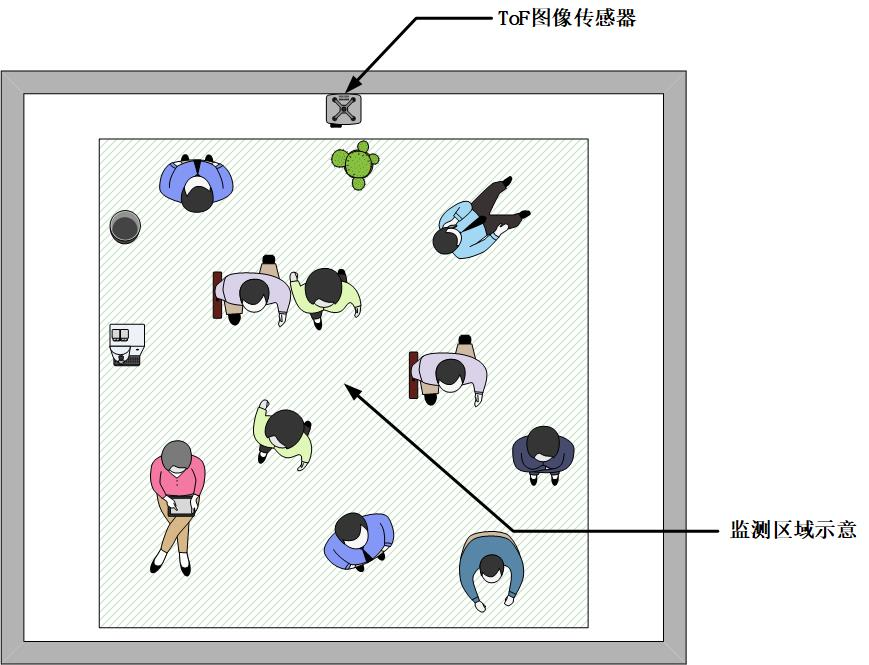
\includegraphics[width=0.67\linewidth]{chap2/surveillance.jpg}
	\caption{\ \ 多目标实时监测系统示意图}
	\label{fig4-1}
\end{figure}
\vspace{3mm}

\section{应用的轻量化模型架构}
\label{sec4-3}
\subsection{整体架构}
本章节应用的模型加速架构主要由两部分组成,第一部分是对前文研究设计的多目标检测神经网络进行轻量化网络结构修改,
并重新输入图像进行训练,通过更改训练模块网络架构获得更少的参数计算同时保证检测模块的精度,获得一个更加高效的、鲁棒的检测网络;
第二部分由tensorrt量化构成,利用半精度浮点或整形数据存储模型权重,将浮点存储运算转换为整型存储运算,通过这种模型压缩技术将检测网络量化,
获得更小的模型尺寸、更低的内存占用和更少的计算量和计算时间。
模型轻量化在保持检测网络准确度基本不变的情况下获得优化后的检测网络,而tensorrt量化模块负责优化整个算法在硬件平台上的计算过程,二者结合获得最佳的算法部署效果。
下面几节将更加详细地介绍每个模块的内容。

\subsection{模型轻量化}

\subsubsection{网络模型计算量指标FLOPs介绍}

FLOPs,指浮点运算数,可以理解为算法的总计算量,包含乘法运算数和加法运算数,是我们用来衡量算法或网络模型复杂度一种通用指标,
神经网络中通常使用 GFLOPs 衡量,为 1e9 FLOPs,即 10 亿次浮点运算。

\subsubsection{ShuffleNet}
ShuffleNet是旷视科技在2017年末提出的一种轻量化网络模型,其注重于神经网络算法在移动端硬件平台上的实现,其核心是利用逐点分组卷积和通道混排操作来实现更小的、计算更少的网络模型。
首先,逐点组卷积是组卷积和点卷积相结合的一种卷积方式,如图 4 - 2 所示,
其中,组卷积是在输入特征图的通道维度执行分组操作,而点卷积则是在 MobileNet 中也有使用的$1\times 1$卷积核大小的卷积,
有升维和降维的效果,但是逐点卷积也存在问题,即其带来的高昂的计算成本,甚至会导致精度的大幅度下降。于是 ShuffleNet 提出利用逐点组卷积,通过保证每个卷积仅作用在对应的输入通道组,
大大减少了计算量,但是随之而来还有信息阻塞的问题,即每个输出结果仅来自于一部分的输入通道。
\vspace{6mm}
\begin{figure}[h]
	\centering
	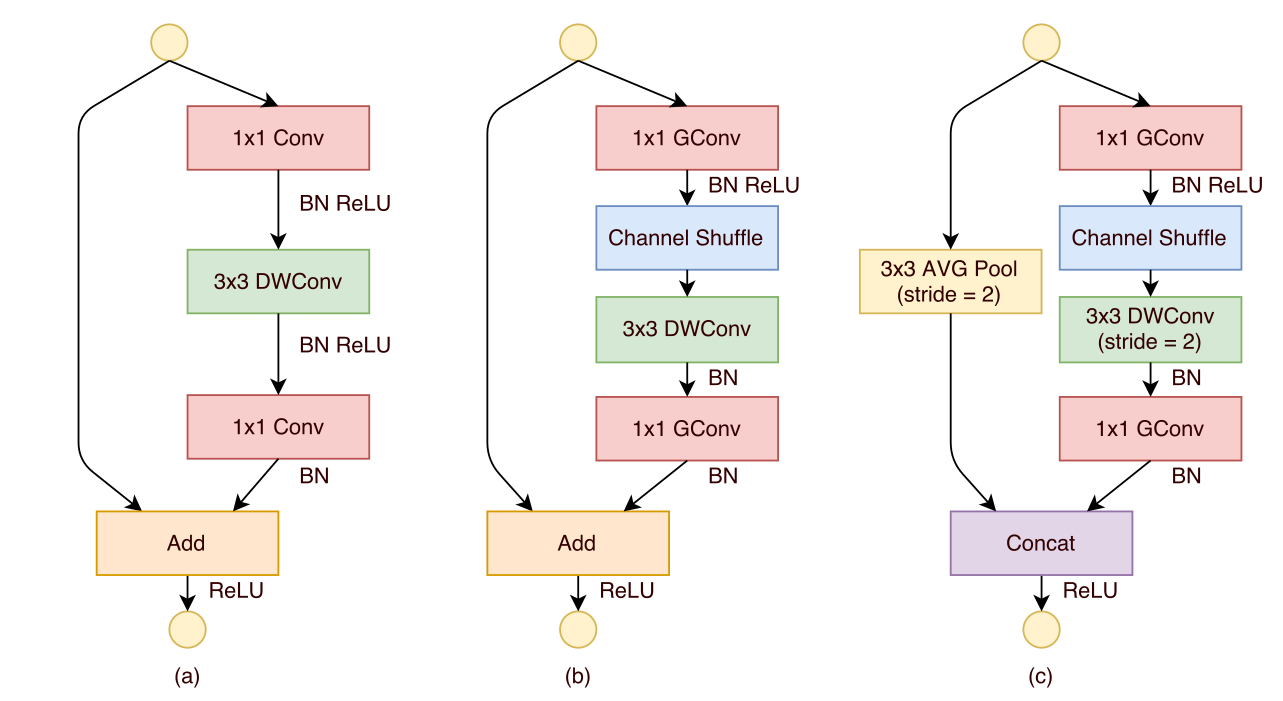
\includegraphics[width=0.67\linewidth]{chap4/Shuffle.png}
	\caption{\ \ 逐点组卷积示意图}
	\label{fig4-2}
\end{figure}
\vspace{3mm}

但是这样会导致不同通道之间的信息无法流动,弱化网络的表达能力,为了解决此问题,
作者提出使用通道混排(图 4 - 3)的方式加强多组卷积层的信息流动,
即在组卷积之后对输出的结果打乱其通道顺序,从而使得不同通道间的特征信息能够随机流动,
增强网络特征提取能力和整体学习能力。
\vspace{3mm}
\begin{figure}[h]
	\centering
	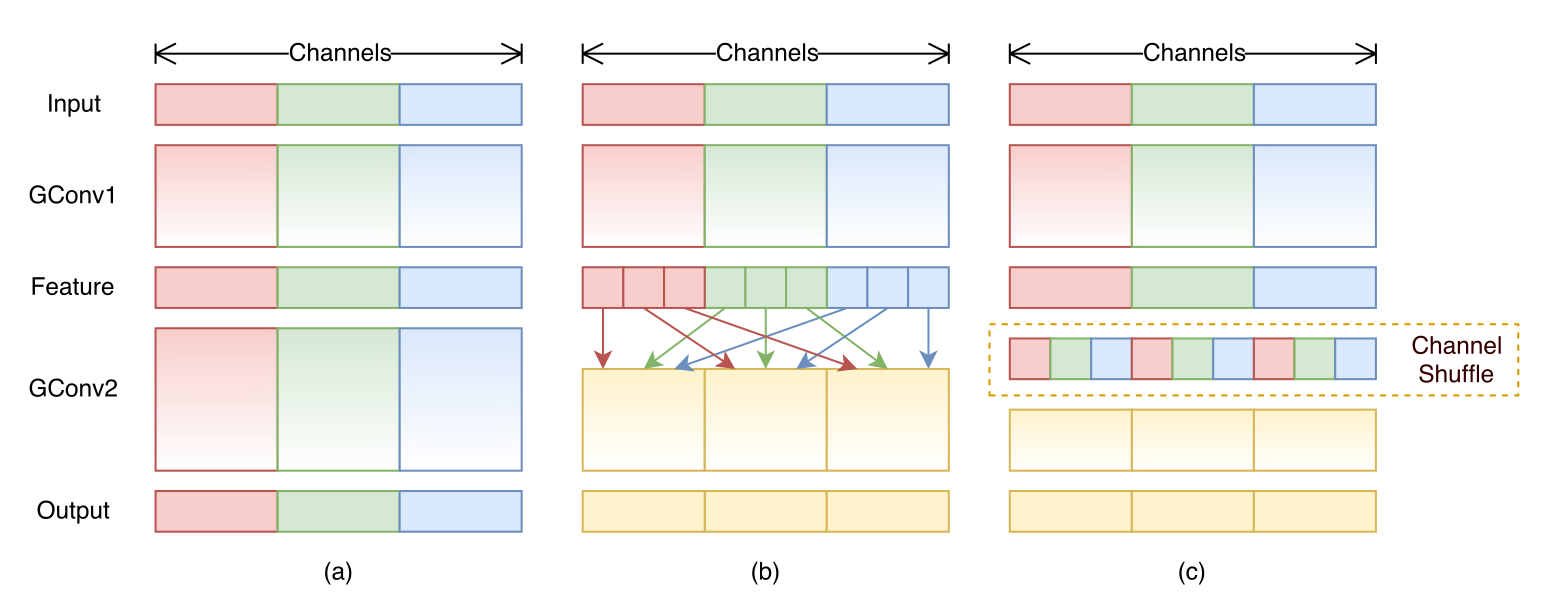
\includegraphics[width=0.67\linewidth]{chap4/Shuffle0.png}
	\caption{\ \ 轻量化网络 $ShuffleNet$ 的通道混排操作过程示意图}
	\label{fig4-3}
\end{figure}
\vspace{3mm}

除此之外,在 ShuffleNet v2 中作者提出了 4 个设计高效网络结构的准则,分别是当输入输出通道数相同时,MAC 内存访问量最小、分组过多的分组卷积会增加 MAC、
碎片化操作对并行操作不友好、逐元素操作带来的内存消耗和耗时不能忽略。
于是 ShuffleNet v2 (图 4 - 4 中 c)将输入一开始就通过通道分离分为两部分,一个分支不变保留原有特征,
\vspace{3mm}
\begin{figure}[h]
	\centering
	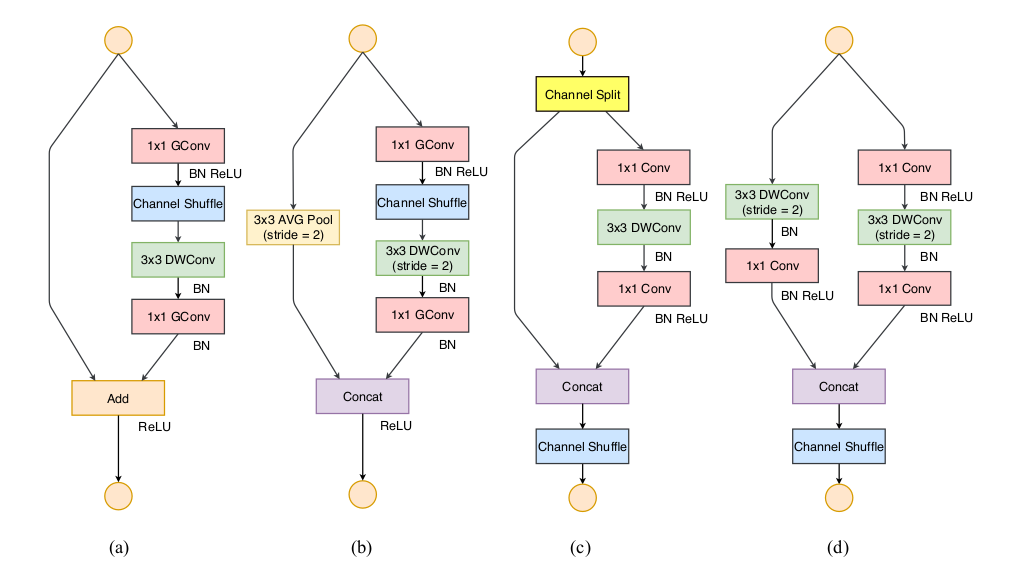
\includegraphics[width=0.67\linewidth]{chap4/Shuffle1.png}
	\caption{\ \ 轻量化网络 $ShuffleNet$ $v2$ 的部分网络结构}
	\label{fig4-4}
\end{figure}
\vspace{3mm}
另一部分$1\times 1$、$3\times 3$深度卷积、$1\times 1$卷积组成,保证输入输出通道相同,之后将两分支拼接经通道混排输出,此结构非常高效。


\subsubsection{MobileNet}
MobileNet 在 2017 年经 Google 提出之后,共经历了三次版本的更新,正如其名,是专注于在移动端设备上应用的轻量级神经网络,
而 MobileNet v1 中其实最主要的变化就是将原来 VGG 网络中的标准卷积层换成了深度可分离卷积。我们知道,可分离卷积有两种,空间可分离卷积和深度可分离卷积,
其中空间可分离卷积就是将一个大的卷积核变成两个小的卷积核,如公式 4 - 1所示,

\begin{equation}
	{\left[ \begin{array}{ccc}
		a & b & c\\
		d & e & f\\
		g & h & i
	\end{array}
	\right ]}
	\ \ =\ \ 
	{\left[ \begin{array}{ccc}
		a \\
		d \\
		g 
	\end{array}
	\right ]}
	\ \ \times\ \ 
	{\left[ \begin{array}{ccc}
		a & b & c
	\end{array} 
	\right ]}
	\label{eq4-1}
\end{equation}
\vspace{3mm}

像是一个 $3\times 3$ 的卷积核就可以分为一个 $3\times 1$ 的卷积核和一个 $1\times 3$ 的卷积核,从而使得乘法运算次数变少,
计算复杂性下降,网络运行速度更快。而深度可分离卷积则是将普通卷积拆分为一个深度卷积(图 4 - 5)和一个逐点卷积(图 4 - 6),
\begin{figure}[htbp]
	\centering
	\begin{minipage}{0.48\linewidth}
		\centering
		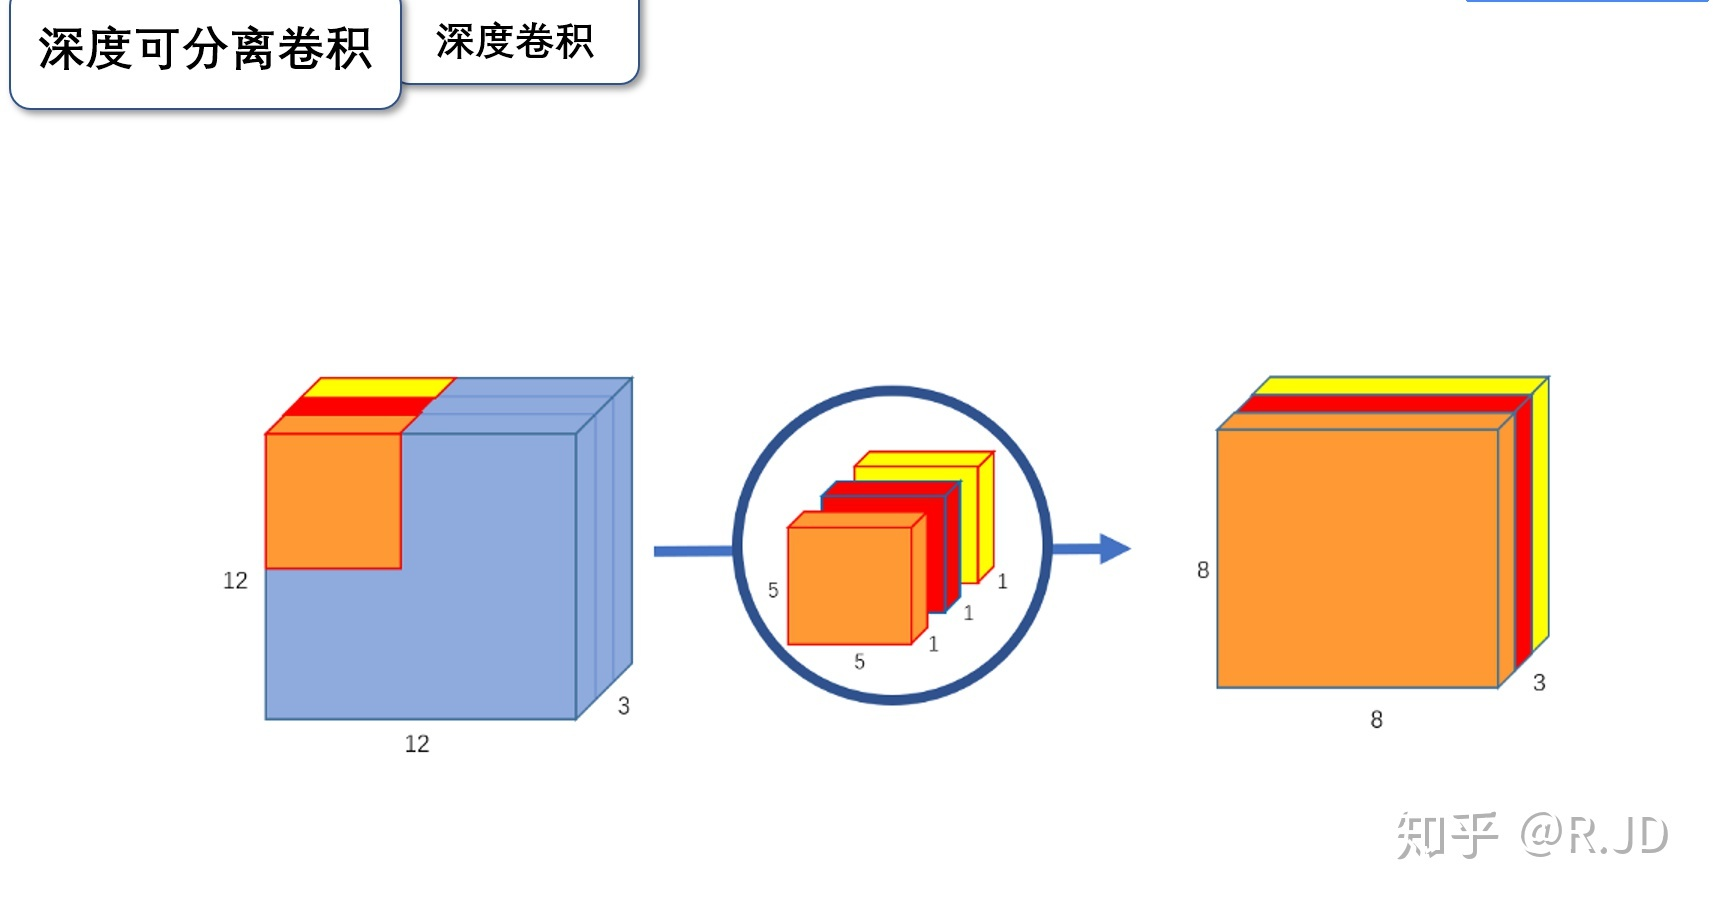
\includegraphics[width=1.0\linewidth]{chap4/Mobile2.jpg}
		\caption{\ \ 深度卷积示意图}
		\label{fig4-5}%文中引用该图片代号
	\end{minipage}
	\begin{minipage}{0.48\linewidth}
		\centering
		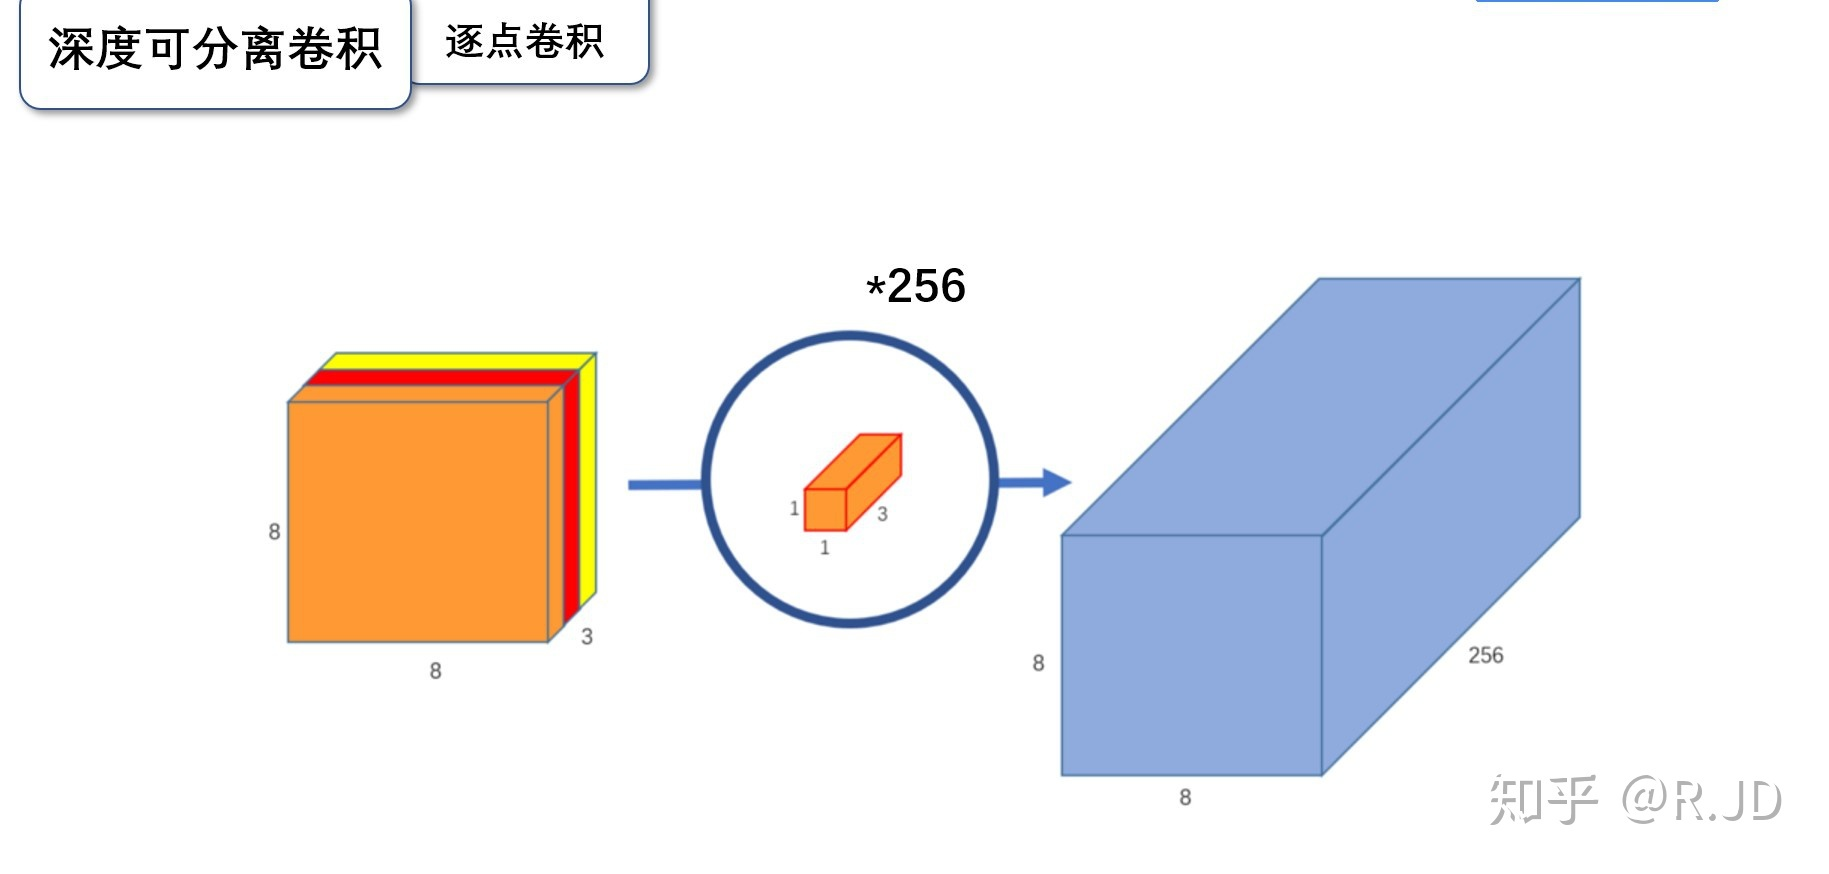
\includegraphics[width=1.0\linewidth]{chap4/Mobile3.jpg}
		\caption{\ \ 逐点卷积示意图}
		\label{fig4-6}%文中引用该图片代号
	\end{minipage}
\end{figure}
不同于标准卷积,我们首先在不改变图像特征深度的情况下,
对每一通道分别进行卷积操作,获得与输入特征图像通道数一致的多个输出特征图,再利用逐点卷积对这些特征图进行升维和降维使其输出的特征图与普通卷积输出一致。
我们使用深度可分离卷积的目标只有一个,那就是使用更少的参数和运算获得与普通卷积差不多的结果。

标准卷积的参数量为:$D_k \times D_k \times M \times N$,而深度可分离卷积的参数量为:$D_k\times D_k \times M$ + $M \times N$,
所以我们可以知道,在相同的权值参数数量的情况下参数大致可以下降为原来的 $\frac{1}{N}$,所以其高效性还是显而易见的。但是之后有人在训练过程中发现会出现卷积核为空的情况,
经研究发现问题出现在 ReLU 这个激活函数上,ReLU 对低维信息做运算过程中会出现信息的丢失,
而高维度信息则几乎不会,所以作者在 Mobilenet v2 中将最后一层的 ReLU 替换成了线性激活函数,除此之外,深度卷积并不会改变输入特征图像的通道数,
而我们已知要在高维度的环境下工作才会有好的效果,于是提出在深度卷积之前利用逐点卷积升维,从而在一个更高维度的特征空间中操作,并且还加入一个 shortcut 结构保留原有特征,
整个过程呈现为先升维再卷积再降维的操作,与 ResNet 相反,故称为倒置残差结构。而 MobileNet v3 是在 2019 年提出的,其在 v1、v2 的基础上引入 SE 模块,
利用结合特征通道的关系来加强网络的学习能力,除此之外还引入了一种的新的激活函数 h-swish(hard swish),其对比 swish 更适用于移动端设备的部署,作者认为随着网络的深入,
应用非线性激活函数的成本会降低,能够更好的减少参数量,因此通过在 v3 网络结构更深的层中使用 h-swish 获得了更好的轻量化效果,并且在最后层加入$1\times 1$卷积核来扩展到高维空间,
可以更好地做预测。我们观察可以知道,MobileNet 花了大量时间在$1\times 1$卷积上,首先,卷积操作实际上就是先乘后加的操作,而计算机操作时的内存是按照行先序的方式存储的,
而一般卷积都是通过 im2col 的方式牺牲大量内存空间将特征图转为大型矩阵然后进行计算,而$1\times 1$卷积的好处在于不再需要此过程,
因为通过$1\times 1$卷积处理后,在物理内存中就已经将其存放为 im2col 处理后的矩阵形式(如图 4 - 7),因此省去了大量数据排列的时间和空间,这也是 MobileNet v3 能如此快的底层原因。
\vspace{3mm}
\begin{figure}[htbp]
	\centering
	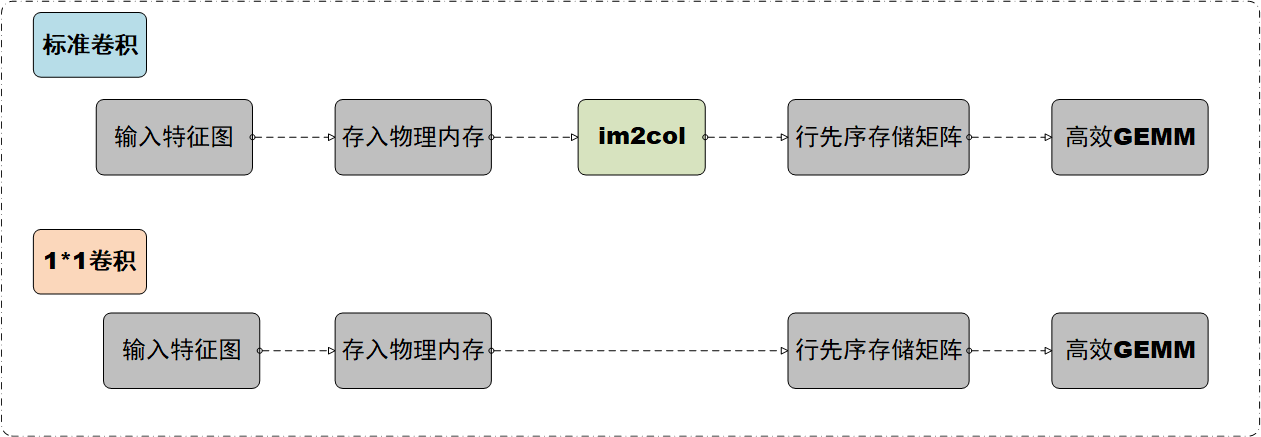
\includegraphics[width=1.0\linewidth]{chap4/Mobile4.png}
	\caption{\ \ $1\times 1$ 卷积对数据处理的简化流程示意图}
	\label{fig4-7}
\end{figure}
\vspace{3mm}


\subsubsection{GhostNet}
GhostNet 是由华为研究团队 2020 年在 CVPR 上发布的一篇对卷积层进行改进的文章,其核心思想是利用 Ghost Module 替换 CNN 网络中的卷积层,从而使整个网络更加轻量高效。
作者发现通过 ResNet 第一组残差处理后的输出特征图中有很多高度类似的特征图,称为 Ghost 对(如图4 - 8),
\vspace{3mm}
\begin{figure}[htbp]
	\centering
	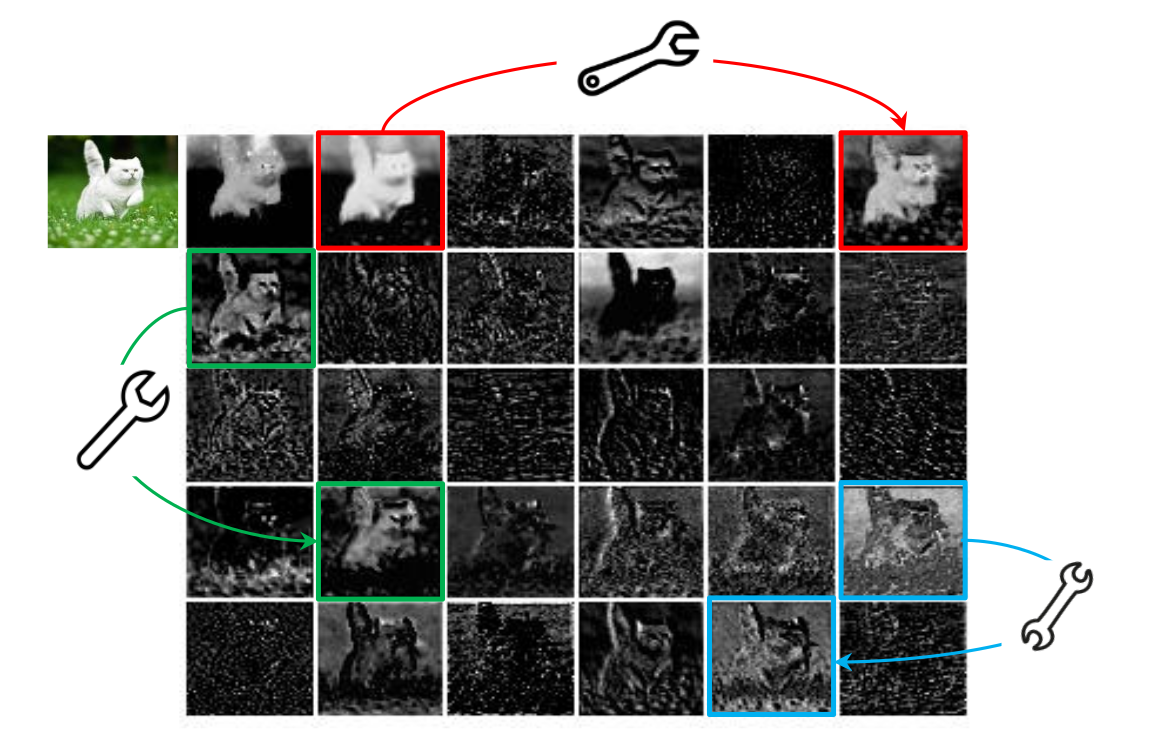
\includegraphics[width=0.67\linewidth]{chap4/Ghost1.png}
	\caption{\ \ 轻量化网络 $GhostNet$ 中的 $Ghost$ 对}
	\label{fig4-8}
\end{figure}
\vspace{3mm}
而传统想法认为这些相似的特征图没有太大意义,但是作者却认为 CNN 的特征提取能力与 Ghost 对的数量正相关,即这种 Ghost 对越多反而效果越好,于是通过 Ghost Module,利用简单的线性操作来获得更多的Ghost对,
最后发现计算量大量减少。Ghost Module首先利用常规卷积得到本源特征图,然后通过线性操作对每一个通道的特征图生成对应的Ghost特征图,
而后将二者拼接输出,作为新的特征图进一步学习,(如图4 - 9)。
\vspace{3mm}
\begin{figure}[htbp]
	\centering
	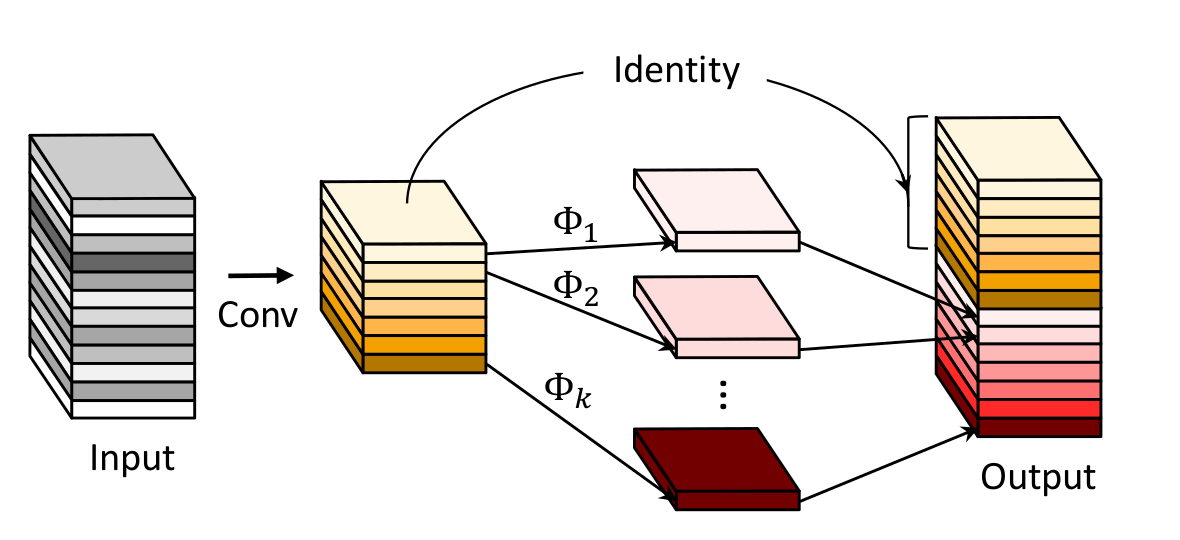
\includegraphics[width=0.67\linewidth]{chap4/Ghost2.png}
	\caption{\ \ 轻量化网络 $GhostNet$ 中的 $Ghost$ $Module$}
	\label{fig4-9}
\end{figure}
\vspace{3mm}

以及Ghost BottleNeck整体的架构就是将Residual Block中的卷积都替换成Ghost Module得到,从而可以很方便地嵌入到其他CNN网络中去(如图4 - 10)。
\vspace{3mm}
\begin{figure}[htbp]
	\centering
	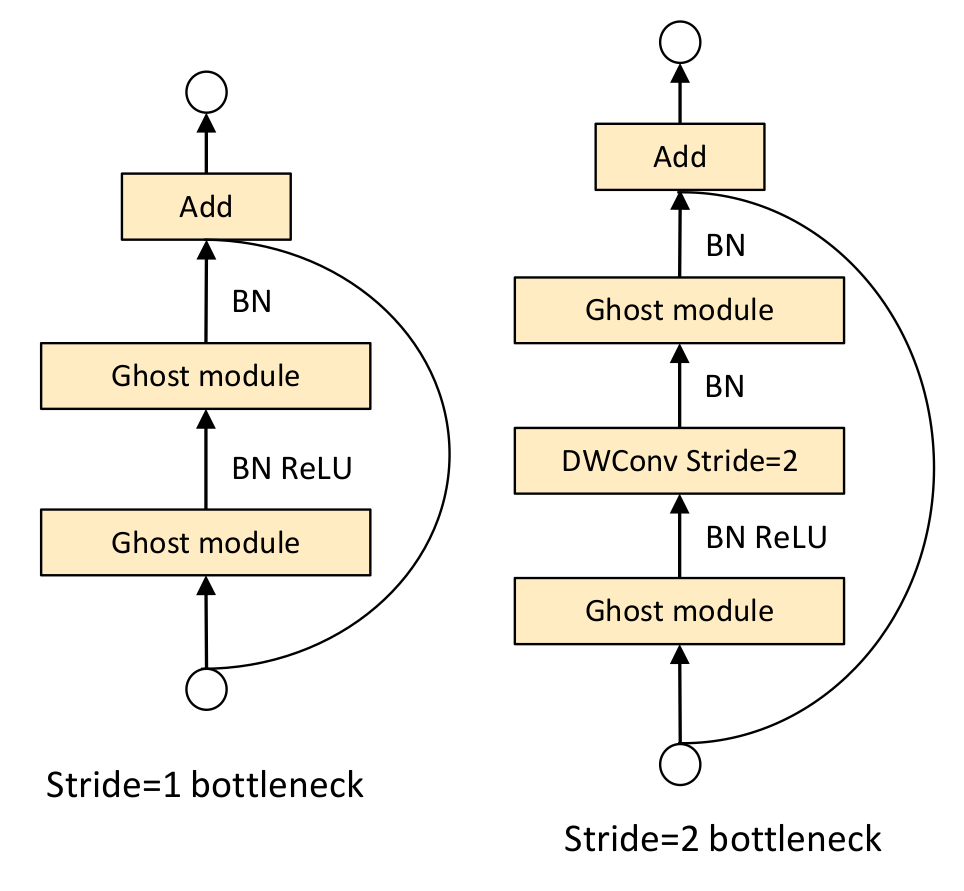
\includegraphics[width=0.67\linewidth]{chap4/Ghost3.png}
	\caption{\ \ 轻量化网络 $GhostNet$ 中的 $Ghost$ $BottleNeck$ 复合模块}
	\label{fig4-10}
\end{figure}


\subsubsection{CA}
CA 为坐标注意力机制,是在 2021 年 CVPR 上发表的一篇文章,它主要针对于通道注意力机制在提升模型性能的同时忽略了空间位置特征的问题,
提出将空间位置信息嵌入到通道注意力中的一种新的移动网络注意力机制。其将通道注意力过程分为两个平行的一维特征处理过程,而后分别沿 2 个空间方向将空间坐标信息合并到特征向量中,
从而在获取空间方向的远程依赖关系同时保留精确的位置信息。且 CA 注意力机制可以应用到大多轻量化网络中去,
向前文提到的 ShuffleNet、MobileNet、GhostNet 等,而且几乎没有额外计算开销,是一种很高效的网络模型插件,文章中也用多项事物检测比较说明此注意力机制的好处。
%\vspace{3mm}
\begin{figure}[htbp]
	\centering
	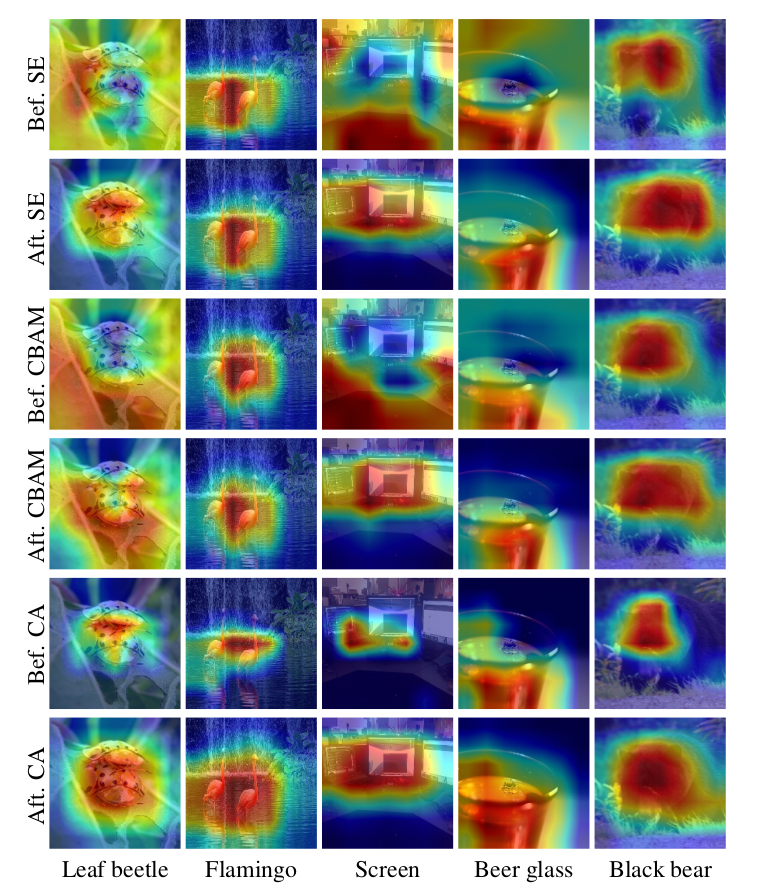
\includegraphics[width=0.67\linewidth]{chap4/CA.png}
	\caption{\ \ $CA$ 注意力机制效果示意图}
	\label{fig4-11}
\end{figure}
%\vspace{3mm}


\subsection{硬件量化加速}
量化是指将某种信号的连续取值近似为有限的多个不同点离散值的转化过程,是一种信息压缩的方法,而对于深度学习神经网络而言,即是对训练好的权重模型进行转化,
将高精度的模型信息使用低精度的模型存储,常规的神经网络模型权重存储精度一般为 FP32(32 位浮点,单精度),而低精度有 FP16(16 位浮点,半精度)和 INT8(8 位定点整数)等数值格式,
目前普遍使用 INT8 量化方式来进行模型压缩,简单来说,就是我们将原来使用 FP32 位浮点数存储的权重和偏置模型现在使用INT8的整数存储,大大减少运算推理过程中的计算复杂度和运算存储量,
是部署到硬件平台的重中之重。且由于深度学习神经网络中中间过程参数和计算量主要发生在卷积层和全连接层,因此我们在量化过程中也是主要针对卷积层和全连接层进行量化。
对于一个卷积层或者全连接层而言(这里以卷积层为例,全连接层处理过程类似):

\begin{equation}
	\operatorname{Conv}\left(\bm{X},\bm{W}\right)=\bm{W}\ast\bm{X},
\end{equation}

其中$\bm{X}$,$\bm{W}$分别表示为当前层的卷积输入特征图和当前层的卷积核权重参数。像之前所说,神经网络中使用FP32的浮点数存储权重和偏置信息,这些信息可近似为连续值,
我们就是要对这些连续值进行定点离散化的处理,从而使用 INT8 的整数格式来存储权重信息,节省内存空间:

\begin{equation}
	\begin{aligned}
	\bm{X}\rightarrow\mathcal{Q}\left(\bm{X}\right)&,\ \bm{W}\rightarrow\mathcal{Q}\left(\bm{W}\right),  \\
	\operatorname{Conv}\left(\bm{X},\bm{W}\right)\rightarrow&\operatorname{Conv}\left(\mathcal{Q}\left(\bm{X}\right),\mathcal{Q}\left(\bm{W}\right)\right),
	\end{aligned}
\end{equation}

其中$\mathcal{Q}\left(\cdot\right)$表示量化函数,用来将权重的连续存储定点离散化为整数存储。依据量化函数Q的不同可以大致分为两种量化方式,一种是线性量化,另一种是非线性量化,取决于量化函数Q线性与否;而依据需要量化的参数类型可以分为两类,一种是权重量化,另一种是权重激活量化,取决于是否量化激活函数值,我们这里主要使用线性量化方式,量化权重值。
通常情况下,线性量化函数可以表达为以下形式(以权重量化为例):

\begin{equation}
	\mathcal{Q}(w)\ =\ s\mathcal{A}(\frac{w\ -\ b}{s})\ +\ b,
\end{equation}

其中$w$为$\bm{W}$中元素,$b$是偏置值,$s$是缩放尺度值,$\mathcal{A}$是$\operatorname{round}\circ\operatorname{clip}$复合函数。其中偏置值$b$的作用是对整个权重分布平移,
控制其所在区间,而缩放尺度值$s$是将$\bm{W}$中的权重值缩放到一个固定区间内,$\mathcal{A}$函数中的$\operatorname{round}$函数作用是离散化输入的连续特征值,而$\operatorname{clip}$函数则是用来将要转化的特征值限制在预定的比特数区间内,
如果是 INT8 就是在 -127 到 127 区间内,必定是 2 的整数次幂。
而根据偏置值$b$的存在与否,又可以将线性量化分为对称线性量化和非对称线性量化,其中对称线性量化的偏置值$b$为零,即只缩放不偏移,
故其量化后零点和特征零点一致,量化后的点对称分布在特征零点周围;
而非对称线性量化中除了缩放还需偏移,于是量化后零点与特征零点不一致,故量化后的点不对称分布在特征零点周围。

由此可见,对称零点通过忽略偏置值$b$,可生成量化后的对称模型,进一步节省参数计算量。一般情况下,由于训练得到的权重参数基本符合均值为零的正态分布,
故对于卷积核权重参数$\bm{W}$采用对称线性量化,而输入特征图通常是上一层输出经激活函数后的值,其分布不符合均值为零的正态分布,故对输入特征图X采用非对称线性量化。
除此之外,我们选取的是训练后量化方式,这种方式使用方便,直接对训练完成的模型权重进行量化,而且由于我们使用的是 TensorRT,TensorRT 针对后端引擎进行加速时使用的是对称量化方式,
维持一致性原则,我们直接选用对称线性量化对权重进行量化。
另一种是非线性量化方式,其量化点之间的间隔不相等,早期使用矢量聚类的方式进行量化,而后又有人提出基于梯度进行优化,通过观察目标函数的梯度下降来确定量化后的点。
虽然非线性量化可以获得很低的量化后位数,但是由于其量化点的无规则性,量化后的模型不能在普适性的硬件平台上进行低位定点运算,因此不使用。
其实还有一种是对数量化方式,通过对两个同底的幂指数进行相乘,从而等价于其指数相加,降低了计算复杂度,但这种方式很少见,也并没有在较好平台上的应用,不建议使用。

\section{实验}
\label{sec4-4}
本节展示了将整个实时监测系统在经过前文涉及的相关处理之后(包括检测模块、追踪模块、模型轻量化和量化模块)在PC和移动端硬件平台上的实现结果,对于整个实时检测追踪系统,
我们在两种不同的场景下进行了开发,分别是实时检测追踪系统以及区域内人流量监控系统,二者共同基于整个检测追踪框架,在特定的场景下进行了特定的算法处理从而达到不同的监控目的。

\subsection{实验设置}
\label{sec4-4-1}
本章节实验基础设置为:

\textbf{硬件设施信息}。
置于头顶的深度图像传感器Kinect v2一台、PC一台、开发板一块;

\textbf{软件平台版本信息}。
CUDA 版本为 10.2.89、cuDNN 版本为 7.6.5、64 位 Ubuntu 18.04.6 LTS,且所有实验皆在 Pytorch 框架下完成;

\textbf{实验算法模块设置}。
本文实验分为两个模块,首先是多目标检测模块,使用 YOLOv5 检测器,先将 YOLOv5 在 COCO 数据集上预训练,然后在前文提到的 Kinect v2 数据集上训练,
输入图像尺寸为$512\times 424 \times 3$,epochs为 300,batch size为 16,初始学习率为 0.1,
使用 YOLOv5 训练流程,包括多尺度训练等,并采用动量为 0.9 的随机梯度下降法训练,其中指标中的帧率可以反映出模型前向推理时间长短,且包括图片的预处理和算法处理后处理输出的时间。

\subsection{网络轻量化效果对比实验}
\label{sec4-4-2}
我们共选用几种不同方式的网络轻量化方式来进行对比实验,从中选择最适合我们的方案进行下一步实验。其中包括ShuffleNet、MobileNet、GhostNet、CA四种不同方式,
对于每一种轻量化模型方法我们都对网络模型进行了修改并重新预训练,其轻量化对比结果如下(我们选取网络层数、参数量、浮点运算数、帧率四个不同角度来进行对比):
其中PC配置为:Intel(R) Core(TM) i7-9700 CPU @ 3.00GHz * 8、48.0GB内存、GeForce GTX 1080 Ti GPU,GPU单元 3584 个。
如图所示是我们在实验过程中修改网络模型后进行重训练的检测结果对比,可以看到ShuffleNet对我们的检测网络效果轻量化效果最佳,
因此我们之后的具体实现中都选用ShuffleNet作为模型轻量化的第一步,将训练好的检测网络通过ShuffleNet进行参数减少提高移植的鲁棒性。

\begin{table} [htpb]
	\begin{center}
		%\setlength{\belowcaptionskip}{3mm}
		\caption{\ \ 多目标检测模型不同方式轻量化结果对比示意图}
		\label{table4-1}
		\footnotesize
		%\setlength{\tabcolsep}{1.8pt}
		\begin{tabular}{llrrrrrrr}
			\hline
			\multirow{1}*{模型种类} & \multirow{1}*{是否应用 GPU } & \multirow{1}*{网络层数} & \multirow{1}*{参数量} & \multirow{1}*{浮点运算数(FLOPs)} & \multirow{1}*{帧率(FPS)}\\
			\hline \hline
			% $\checkmark$
			ShuffleNet & \ \ \ \ \ \ \ \ \ \ \ - & 181 & 4518 & 0.1G\ \ \ \ \ \ \ \ \ \ \ \ \ \ \ \ \ \ \  & 19.53\ \ \ \ \ \ \ \ \ \ \ \ \ \ \ \ \ \ \ \\
			ShuffleNet & \ \ \ \ \ \ \ \ \ \ \ $\checkmark$ & 181 & 4518 & 0.1G\ \ \ \ \ \ \ \ \ \ \ \ \ \ \ \ \ \ \  & 40.06\ \ \ \ \ \ \ \ \ \ \ \ \ \ \ \ \ \ \ \\
			MobileNet & \ \ \ \ \ \ \ \ \ \ \ - & 319 & 567436 & 0.8G\ \ \ \ \ \ \ \ \ \ \ \ \ \ \ \ \ \ \  & 16.61\ \ \ \ \ \ \ \ \ \ \ \ \ \ \ \ \ \ \ \\
			MobileNet & \ \ \ \ \ \ \ \ \ \ \ $\checkmark$ & 319 & 567436 & 0.8G\ \ \ \ \ \ \ \ \ \ \ \ \ \ \ \ \ \ \  & 36.59\ \ \ \ \ \ \ \ \ \ \ \ \ \ \ \ \ \ \ \\
			GhostNet & \ \ \ \ \ \ \ \ \ \ \ - & 430 & 19200 & 0.2G\ \ \ \ \ \ \ \ \ \ \ \ \ \ \ \ \ \ \  & 16.22\ \ \ \ \ \ \ \ \ \ \ \ \ \ \ \ \ \ \ \\
			GhostNet & \ \ \ \ \ \ \ \ \ \ \ $\checkmark$ & 430 & 19200 & 0.2G\ \ \ \ \ \ \ \ \ \ \ \ \ \ \ \ \ \ \  & 27.68\ \ \ \ \ \ \ \ \ \ \ \ \ \ \ \ \ \ \ \\
			CA\ \ \ \  & \ \ \ \ \ \ \ \ \ \ \ - & 304 & 18368 & 2.1G\ \ \ \ \ \ \ \ \ \ \ \ \ \ \ \ \ \ \  & 18.27\ \ \ \ \ \ \ \ \ \ \ \ \ \ \ \ \ \ \ \\
			CA\ \ \ \  & \ \ \ \ \ \ \ \ \ \ \ $\checkmark$ & 304 & 18368 & 2.1G\ \ \ \ \ \ \ \ \ \ \ \ \ \ \ \ \ \ \  & 28.45\ \ \ \ \ \ \ \ \ \ \ \ \ \ \ \ \ \ \ \\

			\hline
		\end{tabular}
	\end{center}
\end{table}


\subsection{监测系统对比实验}
\label{sec4-4-3}
实验中我们通过 ROS 调用深度图像传感器并通过不同硬件平台处理图像再将结果显示出来,将整个实时监测系统搭建起来完成监测任务,我们首先在 PC 上实现了整个监测系统,
之后在移植开发板的过程中发现由于算力的下降,实时监测效果并不能很好的达成,故通过不同实验找寻最佳模型轻量化方案以及 TensorRT 量化方案,将整个网络轻量化后移植到开发板上,
最终达成实时监测效果,以下是不同实验结果的对比和相关指标。
移动端硬件平台为 Nvidia jetson Xavier 开发板,显存和内存共用 32 GB,GPU 单元 512 个。

\begin{table} [htpb]
	\begin{center}
		%\setlength{\belowcaptionskip}{3mm}
		\caption{\ \ 实时监测系统监控帧率对比示意图}
		\label{table4-2}
		\footnotesize
		%\setlength{\tabcolsep}{1.8pt}
		\begin{tabular}{llrrrr}
			\hline
			\multirow{1}*{应用平台} & \multirow{1}*{是否应用 GPU } & \multirow{1}*{网络层数} & \multirow{1}*{参数量} & \multirow{1}*{浮点运算数(FLOPs)} & \multirow{1}*{实时监测帧率(FPS)}\\
			\hline \hline
			% $\checkmark$
			PC &  \ \ \ \ \ \ \ \ \ \ \ - & 192 & 7930 & 0.3G\ \ \ \ \ \ \ \ \ \ \ \ \ \ \ \ \ \ \  & 35.51\ \ \ \ \ \ \ \ \ \ \ \ \ \ \ \ \ \ \ \\
			PC &  \ \ \ \ \ \ \ \ \ \ \ $\checkmark$ & 192 & 7930 & 0.3G\ \ \ \ \ \ \ \ \ \ \ \ \ \ \ \ \ \ \  & 65.06\ \ \ \ \ \ \ \ \ \ \ \ \ \ \ \ \ \ \ \\
			Xavier &  \ \ \ \ \ \ \ \ \ \ \ - & 192 & 7930 & 0.8G\ \ \ \ \ \ \ \ \ \ \ \ \ \ \ \ \ \ \  & 2.4\ \ \ \ \ \ \ \ \ \ \ \ \ \ \ \ \ \ \ \\
			Xavier &  \ \ \ \ \ \ \ \ \ \ \ $\checkmark$ & 192 & 7930 & 0.3G\ \ \ \ \ \ \ \ \ \ \ \ \ \ \ \ \ \ \  & 20.78\ \ \ \ \ \ \ \ \ \ \ \ \ \ \ \ \ \ \ \\
			\hline
		\end{tabular}
	\end{center}
\end{table}


\subsection{实际应用场景下结果展示}
\label{sec4-4-4}
\subsubsection{实时监测系统设计}
本监测系统主要由一个深度图像传感器、一个 Nvidia jetson Xavier 开发板、一块显示屏组成,
% \begin{figure}[htbp]
% 	\centering
% 	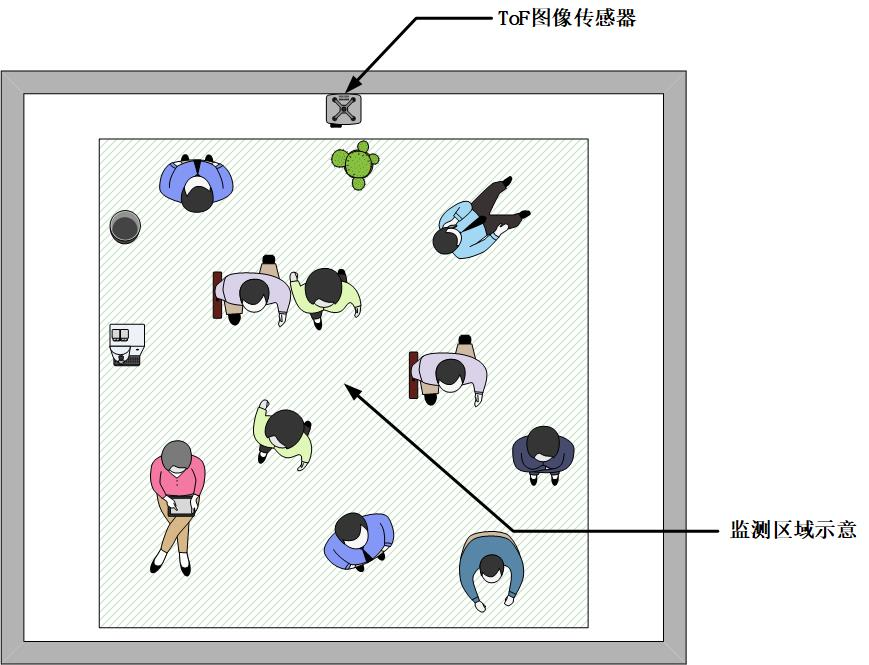
\includegraphics[width=0.67\linewidth]{chap2/surveillance.jpg}
% 	\caption{\ \ 监测示意图}
% 	\label{fig4-12}
% \end{figure}
将深度图像传感器置于天花板上,垂直于地面,场景中由监测主体以及桌椅等杂物构成,整个监测系统通过 ROS 调用深度图像传感器获得图像帧,
然后输入检测神经网络,通过卷积层处理,进行推理,获得位置好分类信息,再利用 DeepSort 实时预测更新轨迹,获得多目标追踪信息并经后期处理标记后显示在显示屏,从而完成整个实时监测系统。

\subsubsection{实时检测追踪系统}
此实时追踪系统主要利用前文提到的监测系统算法框架,在监测过程中可以平稳运行,极小概率产生误判现象,同时并无id-switch现象出现。
如图所示,是监测过程中的截图,由于篇幅形式限制,视频无法排放,请谅解。 

\begin{figure}[htpb]
	\centering
	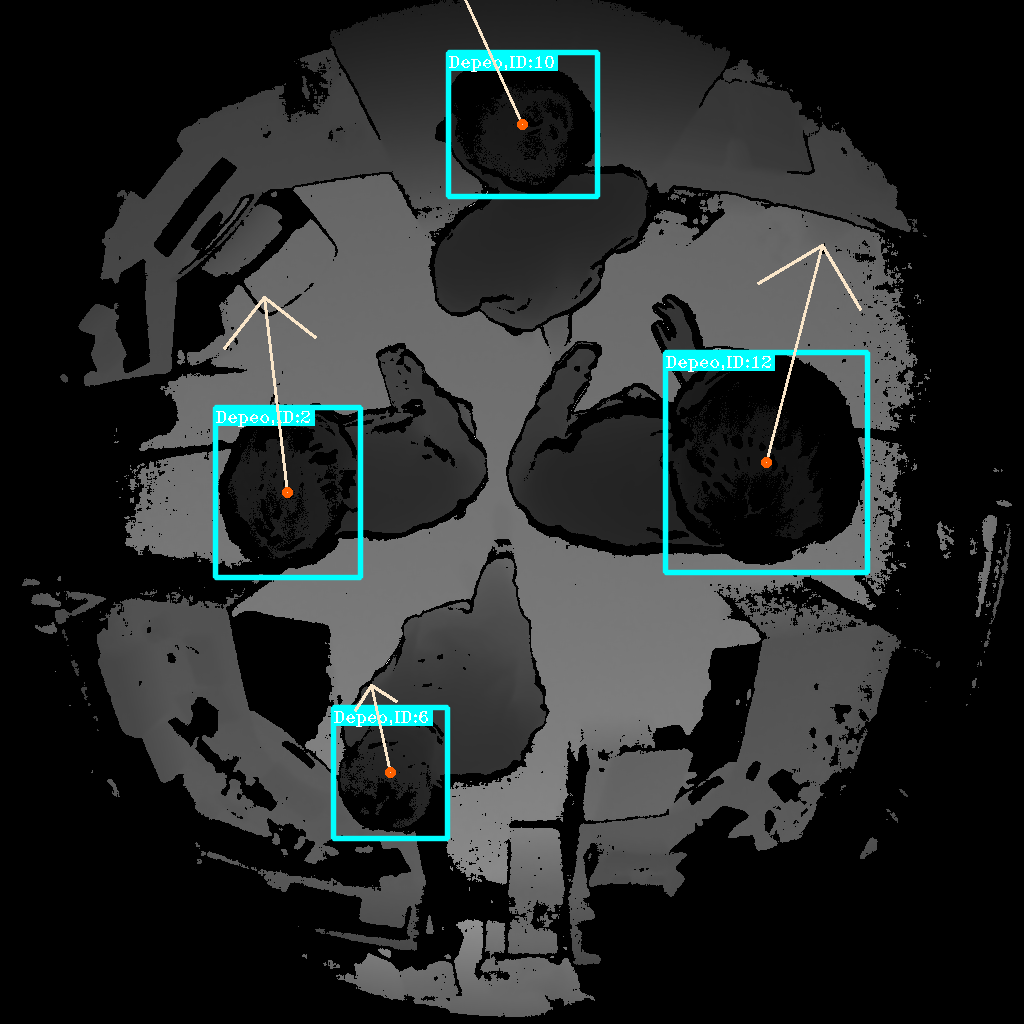
\includegraphics[width=0.48\linewidth]{chap4/v4.png}
	\caption{\ \ 实时检测追踪系统移动端显示结果}
	\label{fig4-12}
\end{figure}

\subsubsection{实时人流量监控系统}
此人流量监控系统主体框架还是相同的检测追踪系统,另外如图所示,
我们设置一条 LOI 线,划分为两个区域,即现实中的园区内和园区外场景,
利用 In 和 Out 代表进入园区内和离开园区外的人数,Existed 代表园区内剩余人数。 

\begin{figure}[htpb]
	\centering
	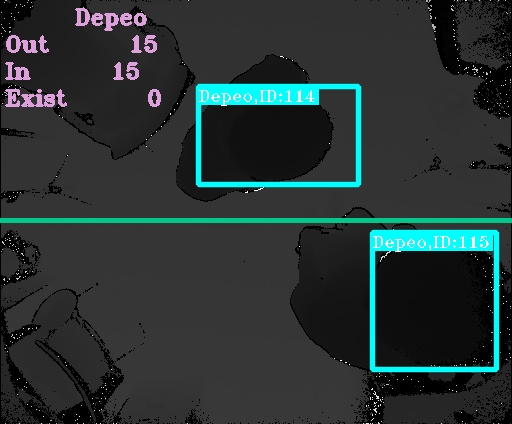
\includegraphics[width=0.48\linewidth]{chap4/v2.jpg}
	\caption{\ \ 实时人流量监控系统移动端显示结果}
	\label{fig4-13}
\end{figure}

研究初始阶段,我们想利用整个轨迹的加速度等信息找出目标经过 LOI 的瞬间并计数,但是在研究过程中发现,如果出现多人同时经过和前后移动的情况以及某个人持续在 LOI 上停留的情况会导致算法产生误判,
故经调整后利用目标在图像中的坐标信息,并通过保留更新前一帧此物体的最后位置坐标和其跨越 LOI 时的坐标变化情况来进行判断,算法流程图如下:
其中$\mathcal{T}$为轨迹集合,$\mathcal{D}$为检测目标集合,
\begin{algorithm}[htpb]
	\floatname{algorithm}{算法}
	\caption{\ \ \ \ \ \ \ \ \ \ 人流量监控计数算法}
	\fangsong
	\hspace*{0.02in} {\bf 输入:\ $\mathcal{T}\ \left\{1, 2, ..., N \right\},\ \mathcal{D}\ \left\{1, 2, ..., M \right\}$ }
	\begin{algorithmic}[1]
		\State 将监测区域的 $\bm{LOI}$ 横坐标设置为 $\bm{x}$;
		\For {$\bm{n}=1$ to $\bm{N}$}
		\State 对\ {\bf $\mathcal{T}$}中轨迹计算 $\bm{Kalman}$ 滤波预测结果;
		\State 经\ $\bm{DeepSort}$ 处理后更新\ {\bf $\mathcal{D}$}中匹配到的 $\bm{id}$ 信息;
		\State 通过\ $\bm{id}$ 定位前一匹配帧中该轨迹的横坐标 $\bm{x_1}$;
		\State 计算匹配的当前检测位置横坐标 $\bm{x_2}$;
		\State 计算\ $ \left(\bm{x} - \bm{x_1}\right) \times \left(\bm{x} - \bm{x_2}\right) $ 是否小于零;
		\State 通过计算结果判定是否此 $\bm{id}$ 目标是否通过 设定的 $\bm{LOI}$;
		\State 基于当前帧的坐标和前一帧坐标的大小关系判定人行走方向;
		\State 并更新\ $\bm{In}$ 、$\bm{Out}$ 和\ $\bm{Existed}$ 对应人数;
		\State 其中\ $\bm{In}$ 和\ $\bm{Out}$ 直接更新,$\bm{Existed}$ 人数由\ $\bm{In}$ 和 $\bm{Out}$ 相减获得;
		\EndFor
		\State \textbf{end for}
		\State 返回处理结果并显示。
	\end{algorithmic}
	\label{algo3}
\end{algorithm}


\section{本章小结}
\label{sec4-5}
本章节通过大量实验研究了多种深度卷积神经网络轻量化方案,并对整体硬件进行底层量化加速,使得整个系统可以有效地在算力有限的开发板上稳定运行并完成监测任务。
综合来看,其实整个模型的轻量化效益还是很强的,尤其在 Xavier 开发板环境下,通过轻量化网络以及硬件量化加速使得整个监测系统的运行速度提高了近十倍,
是对整个轻量化流程的有效验证,提升了整个监测系统的可移植性以及面向智能芯片的发展前景,是对整个研究工作的收尾,也是对未来进一步工作的铺垫。


%%%%%%%%%%%%%%%%%%%%%%%%%%%%%%%%%%%%%%%%%%%%%%%%%%%%%%%%%%%%%%%%%%%%%%%%%%%%%%%%%%%%%%%%%%%%%%%%%%%%%%%%%%%%%%%%%%%%%%%%%%%%%%%%%%%%%%%%%%%%%%%%%%%%%%%%%%%%%%%%%%%%%%%%%%%%%%%%%%%%%%%%%%%%%%%%%%%%%%%%%%%%%%%%%%%%

\chapter{总结与展望}
\label{chap5}
\section{全文总结}

深度卷积神经网络在生活中各个领域所取得的成功不言而喻,在生活中随处可见相关应用,但是普遍的图像处理需要RGB图像,会暴露过多的人体外观特征信息,且数据量更大,占用内存更多,物理成本更高,针对相关问题,我们从图像传感器的角度更改传统策略,使用深度图像传感器获得监测信息,从而完美地保护好监测用户的隐私问题,且利用深度卷积神经网络精准地完成多目标检测任务,同时利用实时多目标追踪算法完成监测的轨迹和人流量监控等,除此之外,在我们部署此类算法到移动端和现实应用中的时候,其庞大的计算成本和内存占用空间都为硬件平台的工艺要求带来了巨大挑战,且针对于深度卷积神经网络,已经有很多优秀的方法被提出来使得整个网络模型轻量化或是压缩加速,而我们从不同的角度考虑此问题,对于输入的数据进行尝试,针对所应用的现实场景,提出了相应的解决方案。这里将本文的研究内容和主要贡献总结如下:

(1)提出一种基于顶部视角深度图像特征的多目标检测网络框架。本文通过研究发现,基于RGB的三通道图像相比与深度图像传感器的单通道图像数据量更多,使用深度图像可以使每一帧的数据量成倍数减少,从而神经网络在处理过程中的参数量也随之减少,可以降低算法的内存要求和计算成本,且利用顶部视角的深度图像,可以获得更好的人头高度变化,网络学习特征更加独特,检测网络学习过程中针对高度特征进行回归,从而在推理过程中只需要深度信息即可检测出相应目标。

(2)提出一种基于顶部视角深度图像特征的多目标实时追踪算法。在本文研究过程中,我发现利用顶部视角的深度图像已经可以避免大部分物体间遮挡情况,从而不再需要单独考虑造成多目标追踪场景下的id-switch现象,而相关多目标追踪算法中会有冗余的计算过程,因此我们通过选择避免不必要的计算步骤来进一步减少追踪过程中的计算量,降低整体算法的复杂度,提高实时监测系统的可移植性,也是为之后的监测系统实际应用化做出铺垫。

(3)应用一种模型轻量化框架和硬件量化加速相融合的方式将算法计算量减少并成功部署到算力有限的硬件开发板环境中,完成整个端到端实时监测系统的设计和开发。在此部分研究过程中,我们主要是利用已有的神经网络模型轻量化方案和硬件量化加速方案结合,将整个实时监测算法的计算复杂度和内存占用率降低,成功部署到算力较差的移动端开发板上去,而且对整个系统做多种变形应用于现实场景,达成较好的监测效果,是算法实现的较好研究方式,争取让算法落在实地,真正有用。

\section{工作展望}

回过头来看整个研究过程,其中可改进的地方还是有很多的,不过因为时间和精力缘故,借此将一些未来可能继续深入研究的看法拙现:
首先,对于多目标检测神经网络,是否能在保持隐私的同时添加更多关键信息帮助冲破目标检测的精确度限制,真正地达到一,从而可以完全的信任软件监测,这是一个很矛盾的难题,既要信息少量节省物力成本,又要利用足够多的特征进行精确检测,甚至可以发明新的图像传感器,获得更好的更专用的数据特征用来做目标检测,包括四肢躯干等人类独有的外观特征等,而且,对于网络的结构是否能进一步的优化,从而减少计算量和内存占用,这也是一个突破点,这个角度可以多考虑如何利用少量权重信息对应精确的模型学习特征,例如特殊的编码等匹配方式,这将极大地有助于神经网络在现实生活中的落地,真正的让科学普惠生活和大众。
